\section{System Walkthrough with Screenshots}
\label{sec:screens}

This section shows the running system. Every figure is a screenshot of the web application served from the stored data of the final system (market prices up to 26 October 2026), captured by a script (\texttt{report/capture\_system.py}) driving a headless browser, so the figures can be regenerated and are not edited. The farmer interface is shown at phone width because that is how most farmers will use it; the trader desk is shown at desktop width. Prices are in rupees per quintal unless stated, and every price on screen carries the date it was reported.

\subsection{Farmer interface}
The farmer interface is built around a single question, ``what is my crop worth today, and where should I sell it?''. It has a language switch (English, Kannada, Hindi), a district selector and a bottom navigation bar with Home, Prices and Tools.


\begin{figure}[!t]
\centering
\begin{minipage}[t]{0.485\textwidth}\centering\fbox{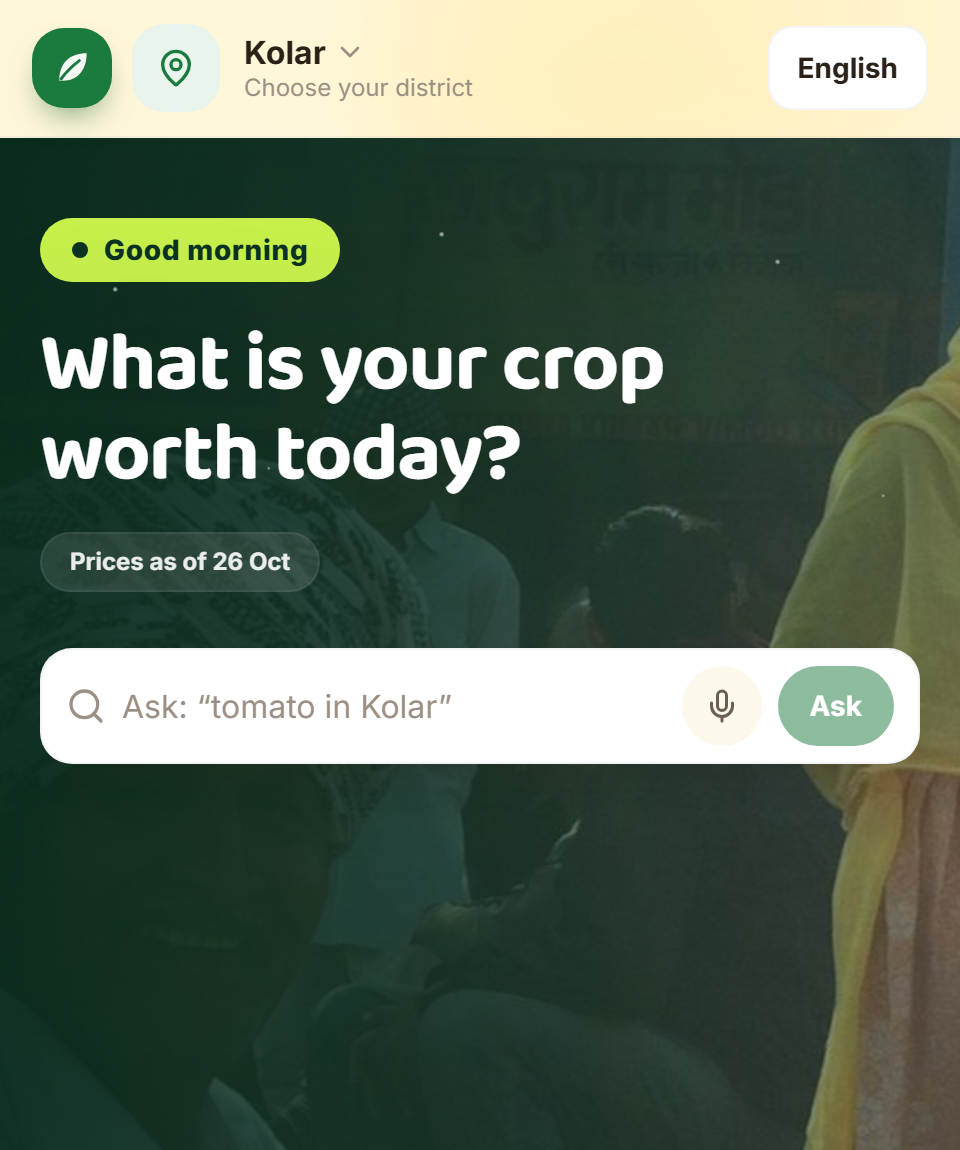
\includegraphics[width=0.94\linewidth,height=9.0cm,keepaspectratio]{figures/shot_f_home.png}}\\[1mm]{\footnotesize (a) Home}\end{minipage}\hfill
\begin{minipage}[t]{0.485\textwidth}\centering\fbox{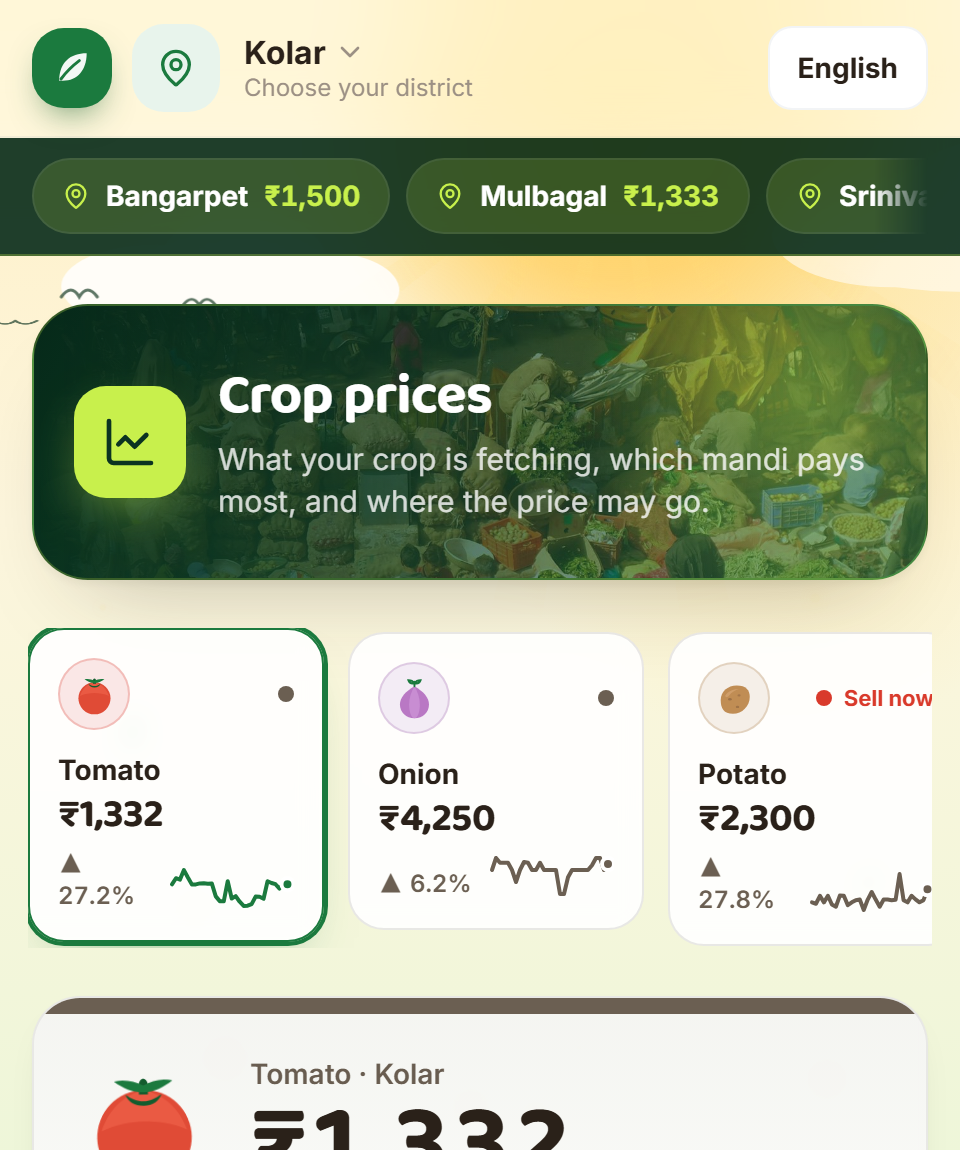
\includegraphics[width=0.94\linewidth,height=9.0cm,keepaspectratio]{figures/shot_f_prices.png}}\\[1mm]{\footnotesize (b) Prices}\end{minipage}
\medskip
\centering \begin{minipage}[t]{0.485\textwidth}\centering\fbox{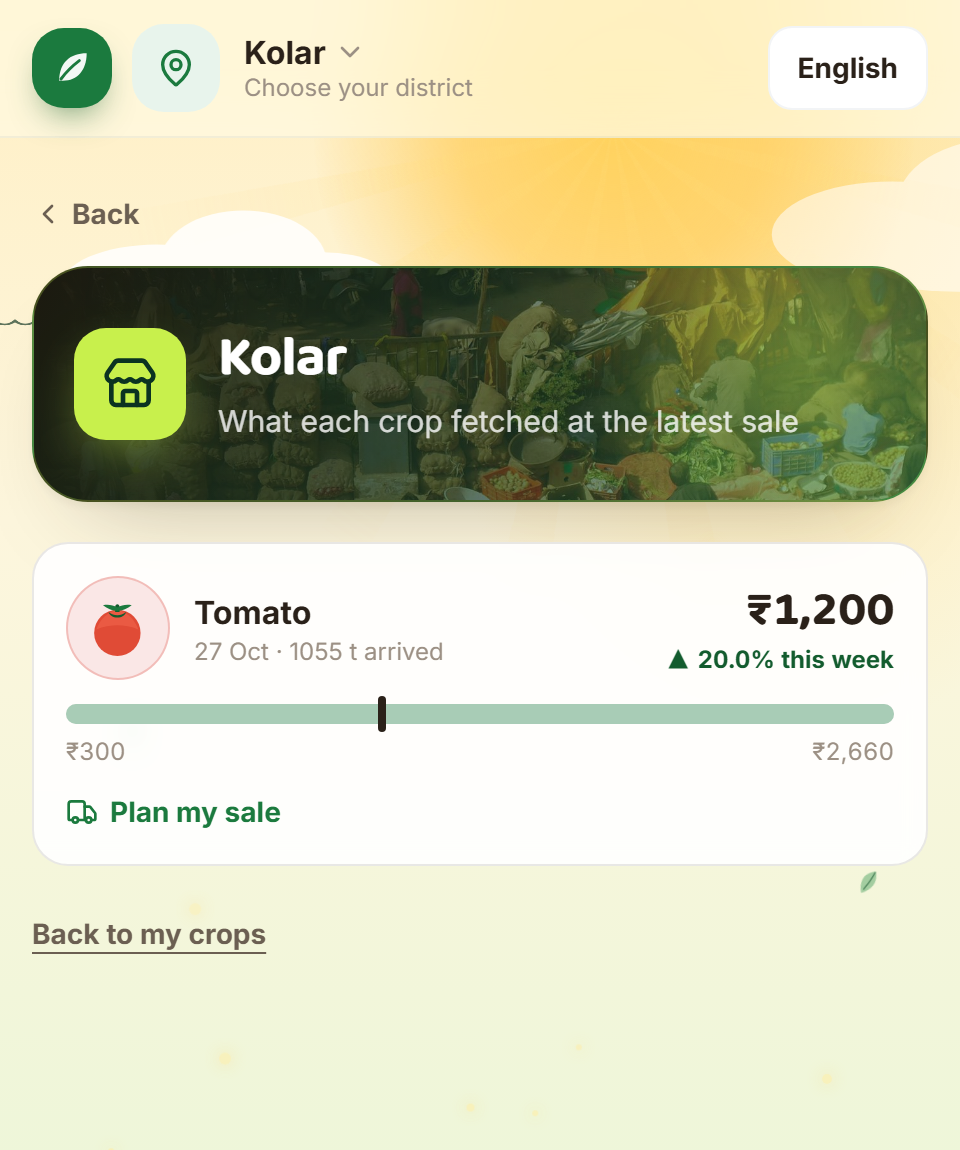
\includegraphics[width=0.94\linewidth,height=9.0cm,keepaspectratio]{figures/shot_f_mandi.png}}\\[1mm]{\footnotesize (c) One mandi}\end{minipage}
\caption{Farmer pages. (a) The home page opens with a plain question, a search box that answers in sentences, and a ticker of the latest prices. (b) The prices page lists the crops with the latest quote, the change over the week and a sparkline. (c) A mandi page shows what each crop fetched there at the latest sale and how many quintals arrived.}
\label{fig:sc-farmer1}
\end{figure}

The home page (Figure~\ref{fig:sc-farmer1}a) deliberately carries no table: the first thing a farmer sees is the question and a box in which to type one in ordinary words. The prices page (b) shows the quote for each crop together with the date of the last report, so a stale price is never presented as today's. The mandi page (c) is the farmer-side view of one market and links to the plan for selling there.


\begin{figure}[!t]
\centering
\begin{minipage}[t]{0.485\textwidth}\centering\fbox{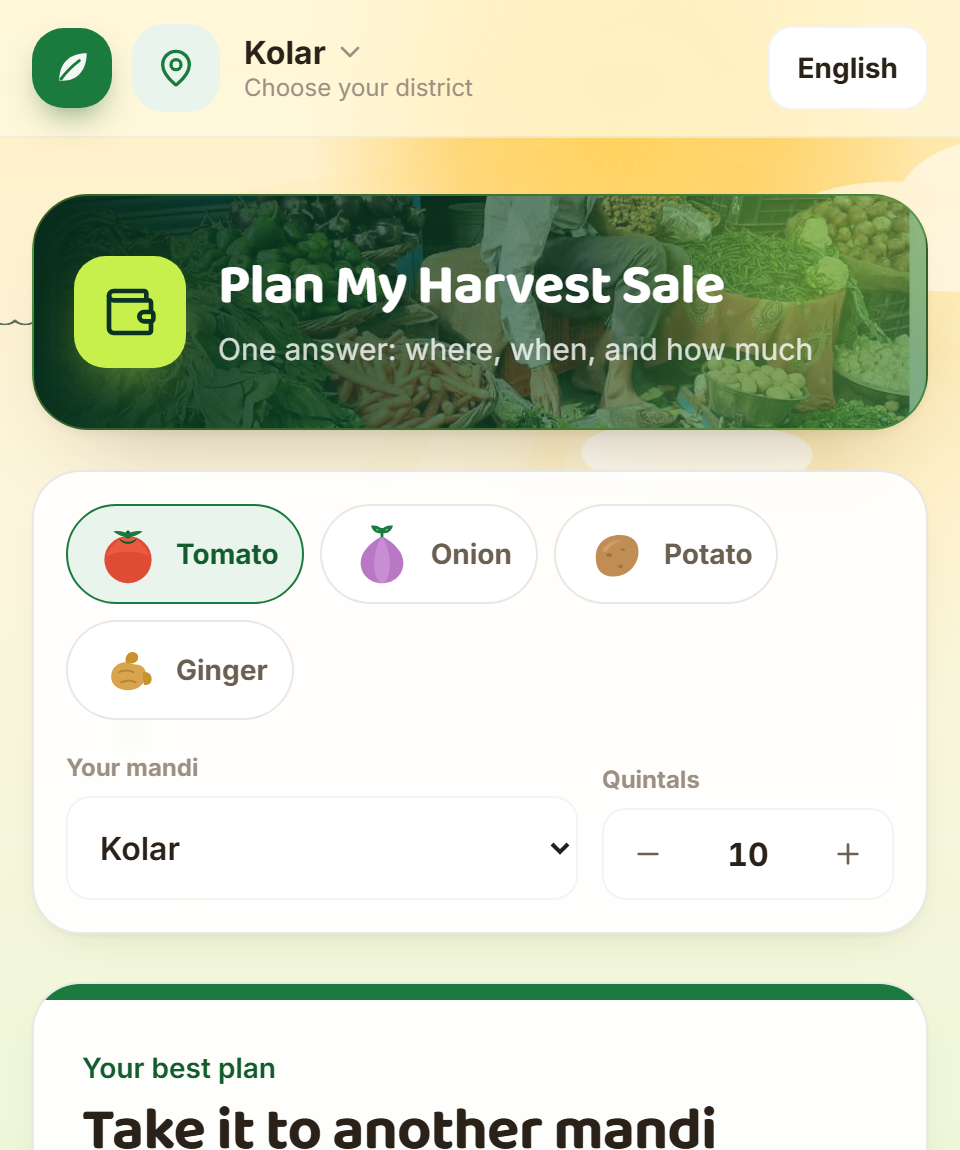
\includegraphics[width=0.94\linewidth,height=9.0cm,keepaspectratio]{figures/shot_f_sellplan.png}}\\[1mm]{\footnotesize (a) Plan my sale}\end{minipage}\hfill
\begin{minipage}[t]{0.485\textwidth}\centering\fbox{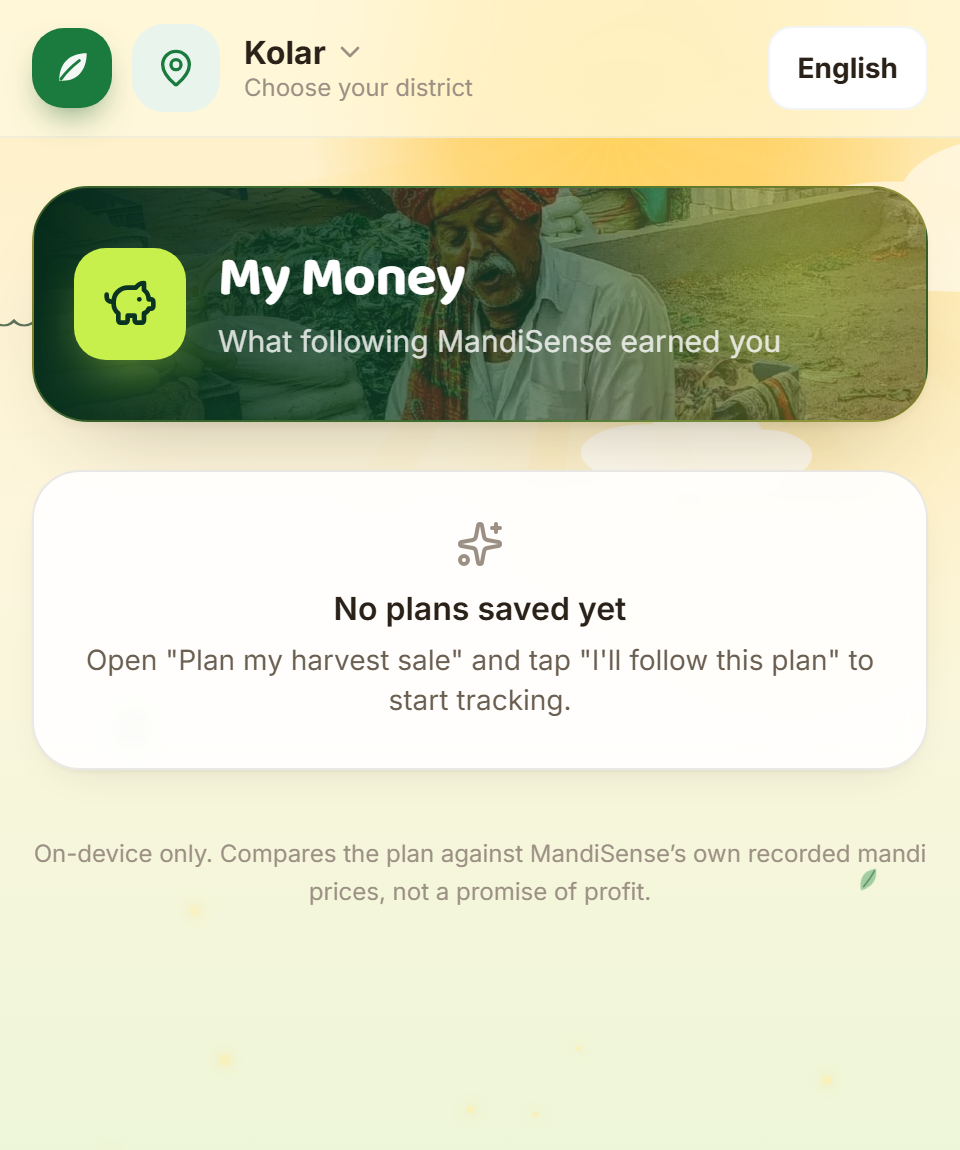
\includegraphics[width=0.94\linewidth,height=9.0cm,keepaspectratio]{figures/shot_f_mymoney.png}}\\[1mm]{\footnotesize (b) My money}\end{minipage}
\medskip
\centering \begin{minipage}[t]{0.485\textwidth}\centering\fbox{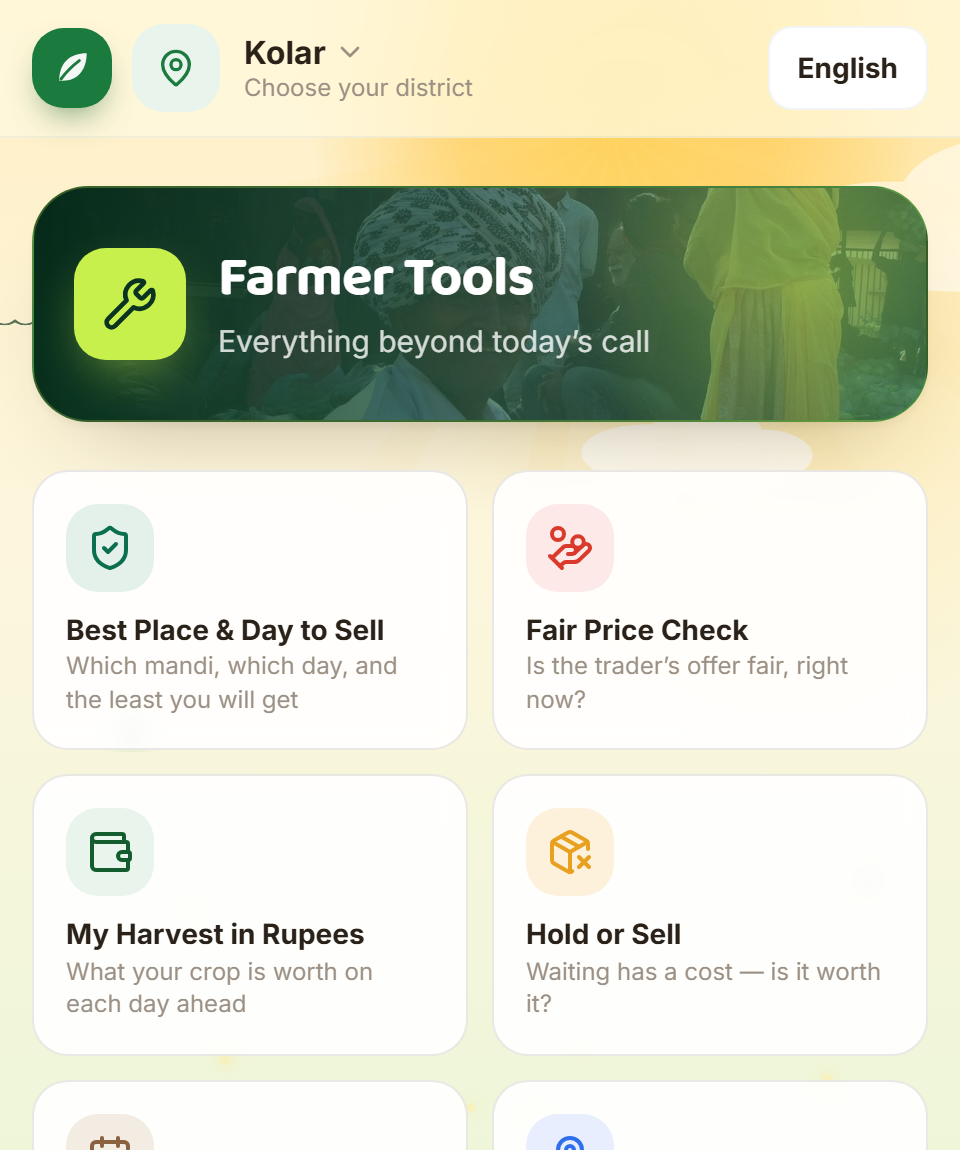
\includegraphics[width=0.94\linewidth,height=9.0cm,keepaspectratio]{figures/shot_f_tools.png}}\\[1mm]{\footnotesize (c) Farmer tools}\end{minipage}
\caption{(a) The sale plan states one recommendation, the amount expected after transport and spoilage, and the day to go. (b) ``My Money'' compares the plans the farmer followed with what the markets recorded; it works on the device only. (c) The tool launcher opens each tool as a sheet over the page.}
\label{fig:sc-farmer2}
\end{figure}

The sale plan (Figure~\ref{fig:sc-farmer2}a) is the product's central screen. It names one market and one day, shows the amount expected per quintal after the cost of moving the crop, and shows the figure the farmer \emph{can count on at least}, which is the revenue floor of Section~\ref{sec:floors}. ``My Money'' (b) keeps the plans on the farmer's phone, so no account or personal data reach the server. The launcher (c) lists the eleven tools whose screens follow.


\begin{figure}[!t]
\centering
\begin{minipage}[t]{0.485\textwidth}\centering\fbox{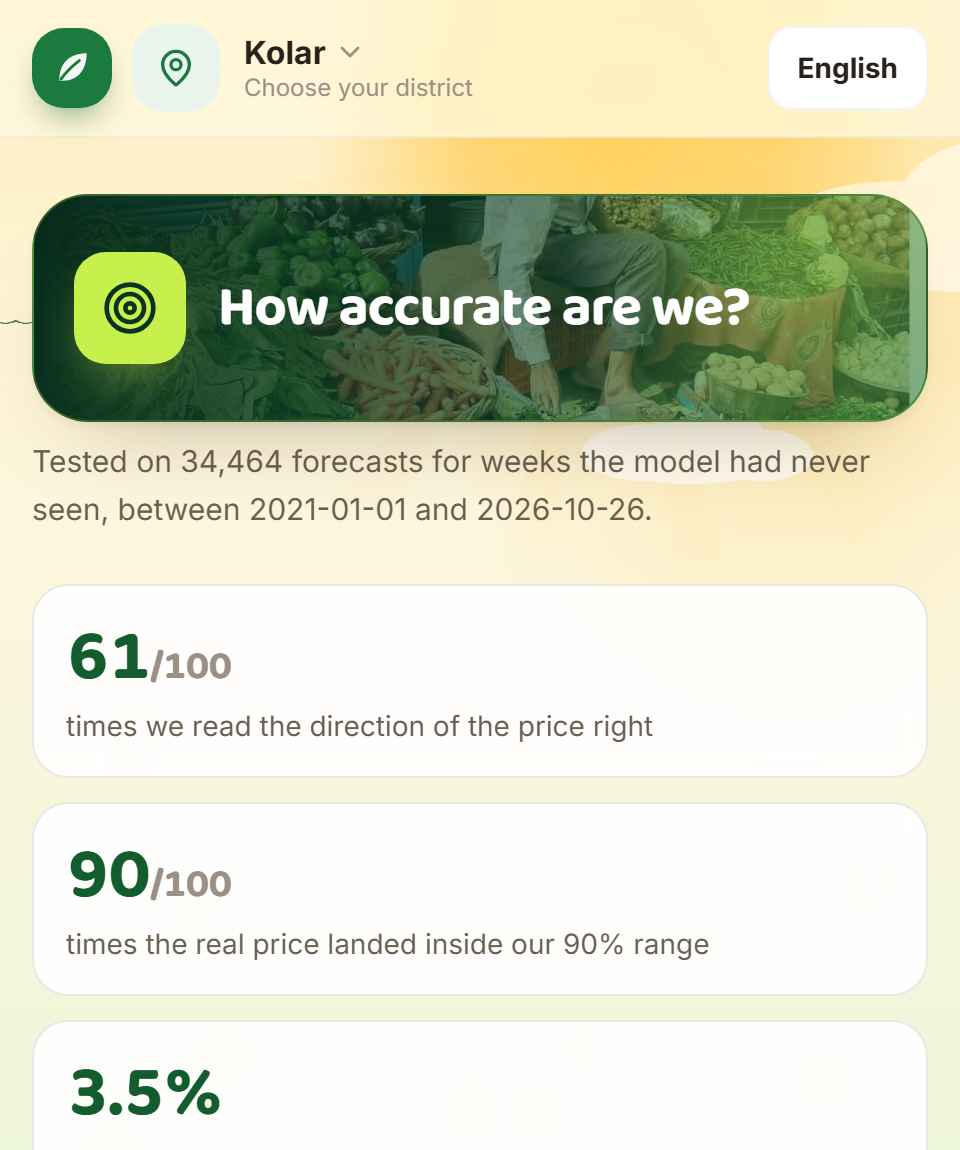
\includegraphics[width=0.94\linewidth,height=9.0cm,keepaspectratio]{figures/shot_f_accuracy.png}}\\[1mm]{\footnotesize (a) How accurate are we?}\end{minipage}\hfill
\begin{minipage}[t]{0.485\textwidth}\centering\fbox{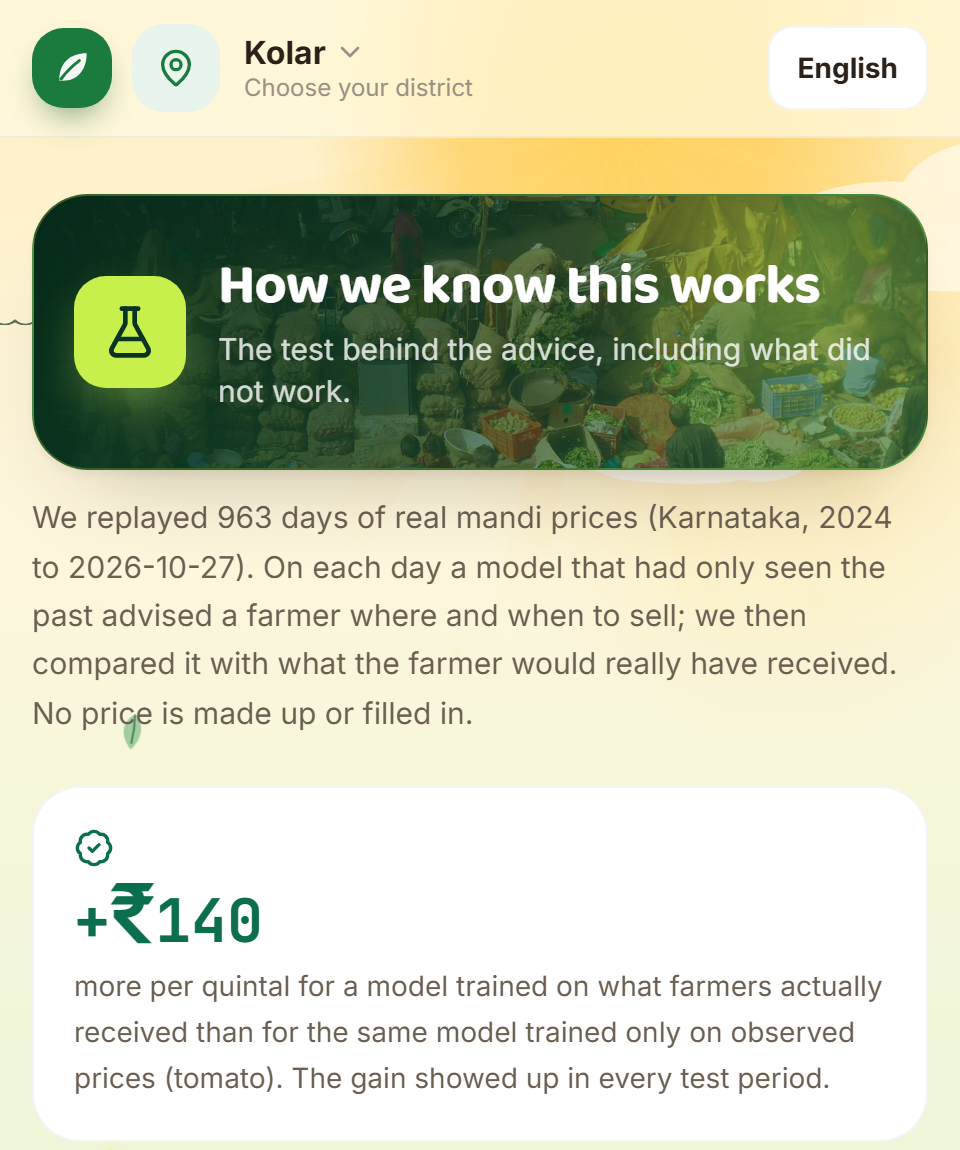
\includegraphics[width=0.94\linewidth,height=9.0cm,keepaspectratio]{figures/shot_f_evidence.png}}\\[1mm]{\footnotesize (b) How we know this works}\end{minipage}
\medskip
\centering \begin{minipage}[t]{0.485\textwidth}\centering\fbox{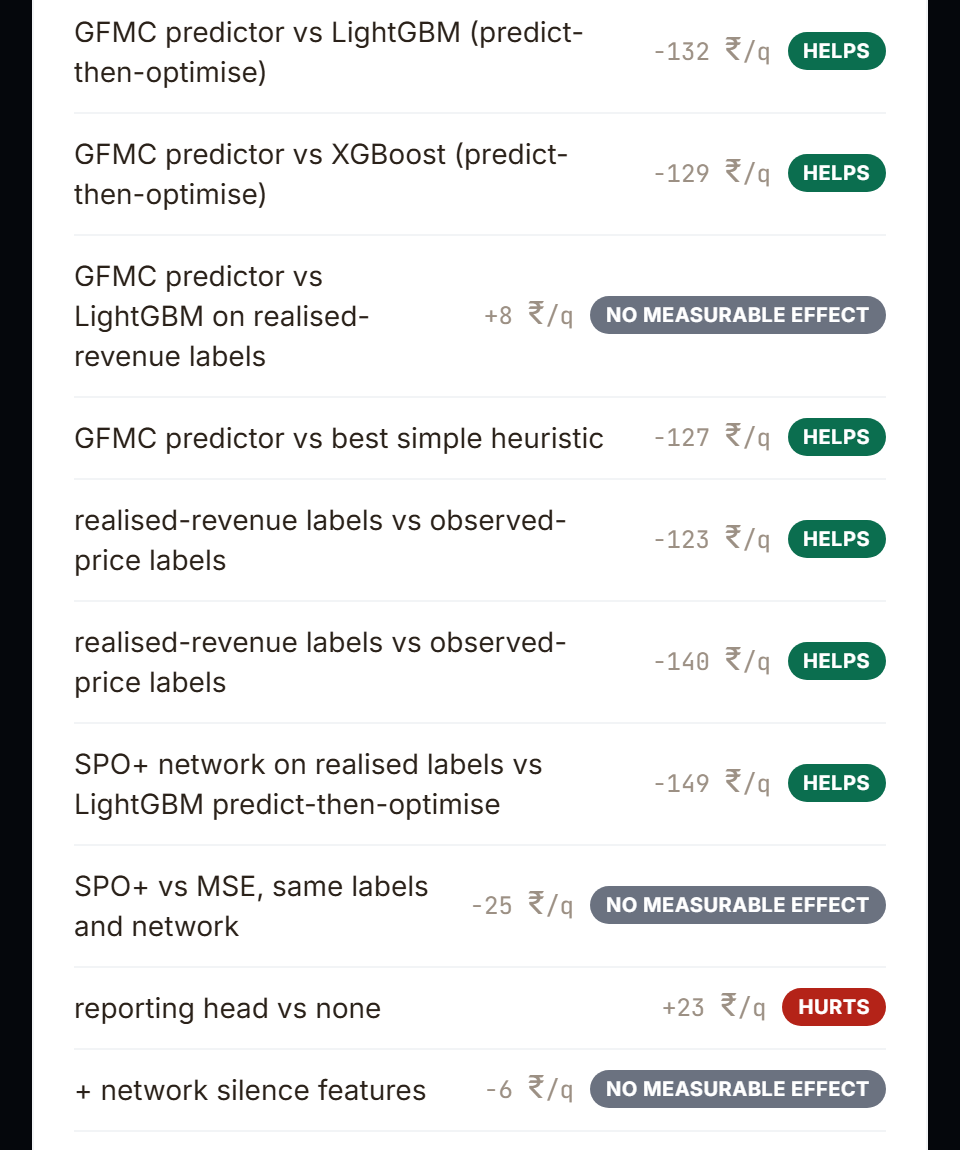
\includegraphics[width=0.94\linewidth,height=9.0cm,keepaspectratio]{figures/shot_f_evidence_b.png}}\\[1mm]{\footnotesize (c) What did not work}\end{minipage}
\caption{The honesty pages. (a) Hit rates by crop and market, on days the system had not seen. (b) The replay: what the method earns against simple alternatives, in rupees, with the seed-to-seed spread. (c) The negative results are listed beside the positive ones.}
\label{fig:sc-farmer3}
\end{figure}

Three pages exist only to let a reader check the system. The accuracy page (Figure~\ref{fig:sc-farmer3}a) reports, per crop and market, how often the advice held on days the system had not seen. The evidence page (b) reproduces the main comparison of Chapter~\ref{ch:results} in plain words and in rupees, and (c) lists what did not help. A product that shows its misses is easier to trust than one that does not.

\subsection{Farmer tools}
Each tool opens as a sheet over the page and answers one question. The sheets below are captured with the sheet in its resting state; the blurred page behind each sheet is cropped away.


\begin{figure}[!t]
\centering
\begin{minipage}[t]{0.485\textwidth}\centering\fbox{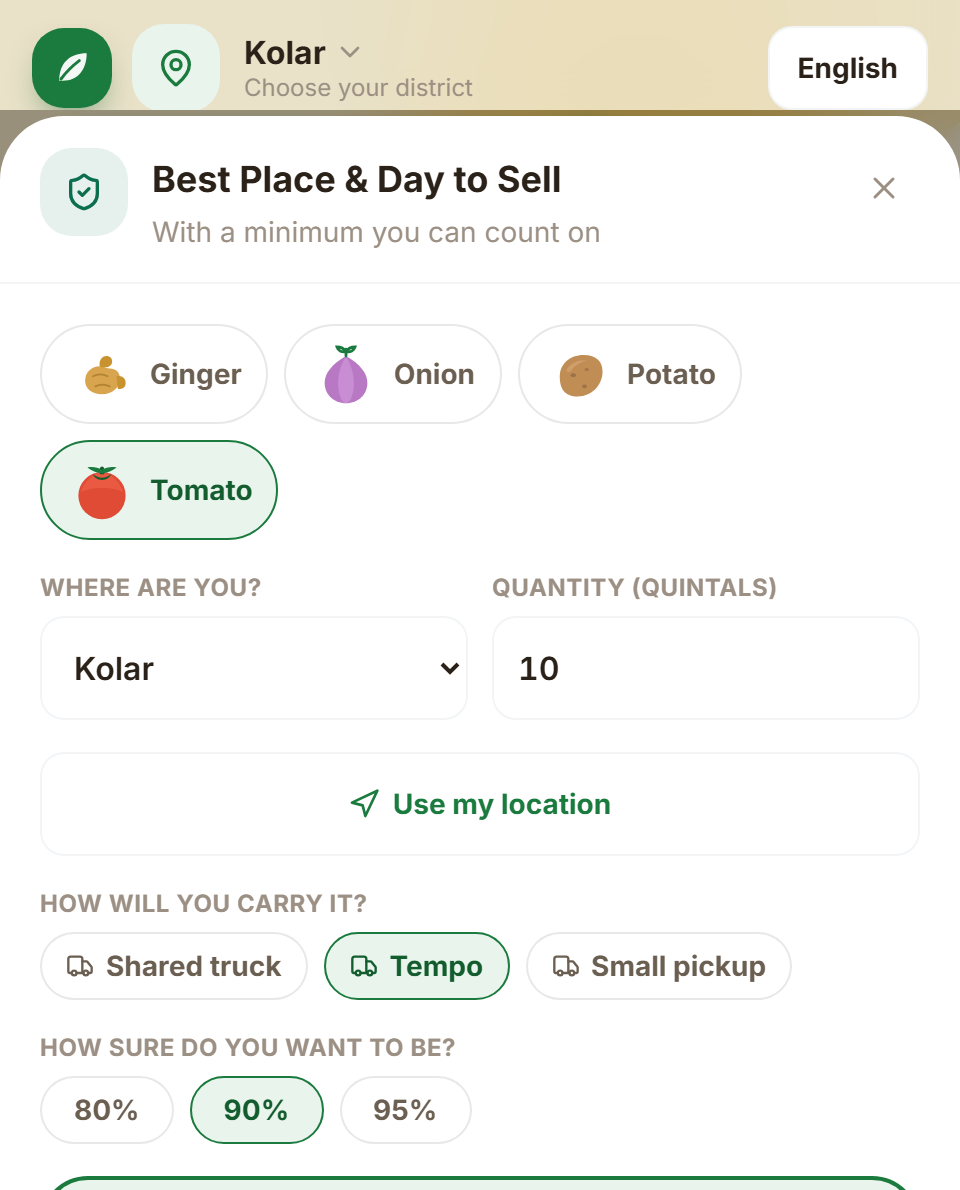
\includegraphics[width=0.94\linewidth,height=9.0cm,keepaspectratio]{figures/shot_t_besplace.png}}\\[1mm]{\footnotesize (a) Best place and day}\end{minipage}\hfill
\begin{minipage}[t]{0.485\textwidth}\centering\fbox{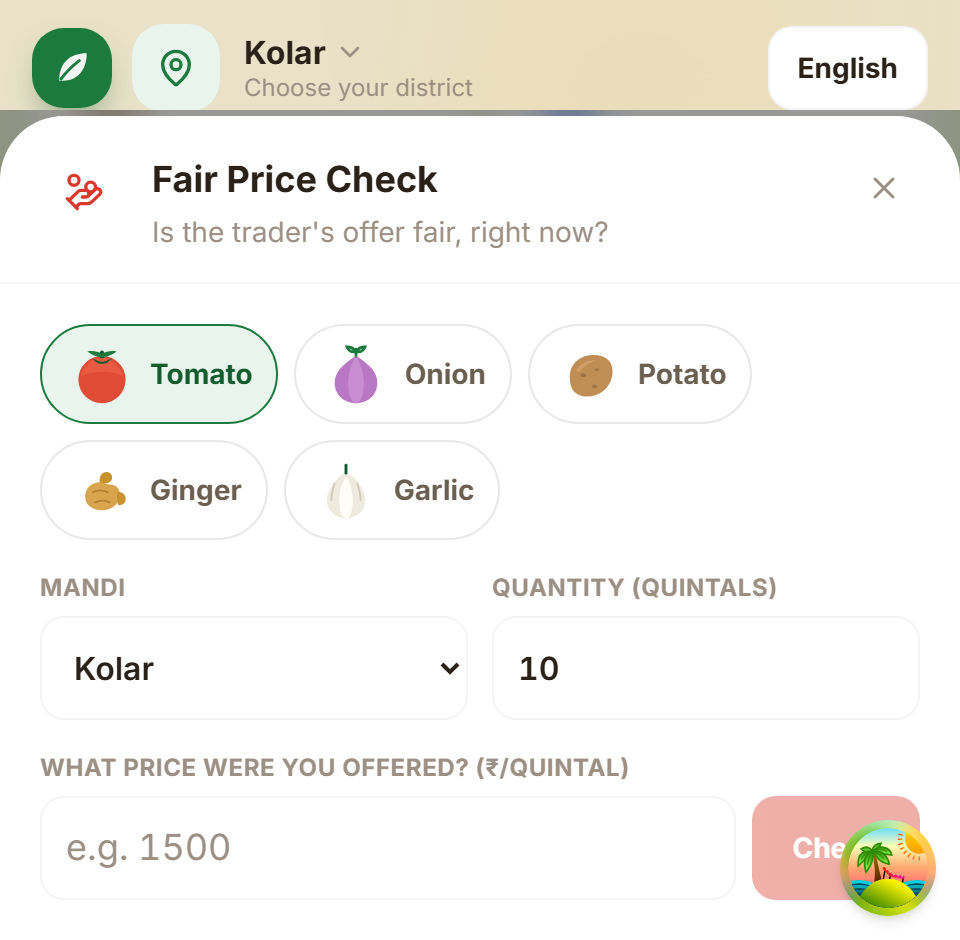
\includegraphics[width=0.94\linewidth,height=9.0cm,keepaspectratio]{figures/shot_t_fairprice.png}}\\[1mm]{\footnotesize (b) Fair price check}\end{minipage}
\medskip
\centering \begin{minipage}[t]{0.485\textwidth}\centering\fbox{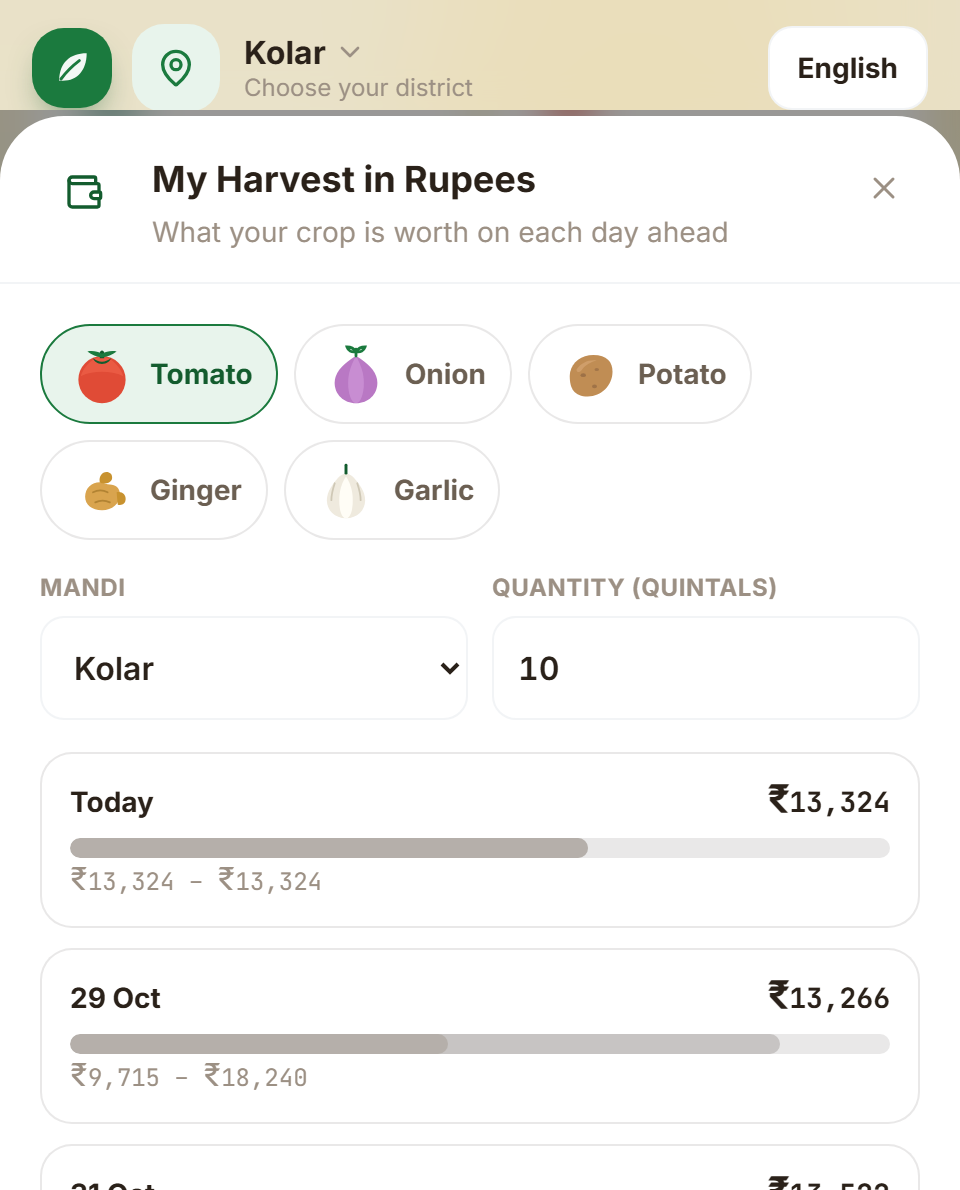
\includegraphics[width=0.94\linewidth,height=9.0cm,keepaspectratio]{figures/shot_t_harvest.png}}\\[1mm]{\footnotesize (c) My harvest in rupees}\end{minipage}
\caption{Selling tools. (a) The recommended market with expected and guaranteed amounts, options to change the vehicle and the confidence, and the next best choices. (b) A check of whether the price a trader offered is fair. (c) The expected value of the crop on each day ahead, after spoilage.}
\label{fig:sc-tools1}
\end{figure}

The Best Place and Day to Sell sheet (Figure~\ref{fig:sc-tools1}a) asks for the district, the quantity, the vehicle and the confidence level (80, 90 or 95\%), and returns the same recommendation as the service of Section~\ref{sec:service-app}, with the cost arithmetic one tap away. The fair-price check (b) takes the offer a trader made and places it against the distribution of recent prices. The harvest sheet (c) lays the next days side by side as a bar for each, with the expected net value, so the farmer sees what waiting costs.


\begin{figure}[!t]
\centering
\begin{minipage}[t]{0.485\textwidth}\centering\fbox{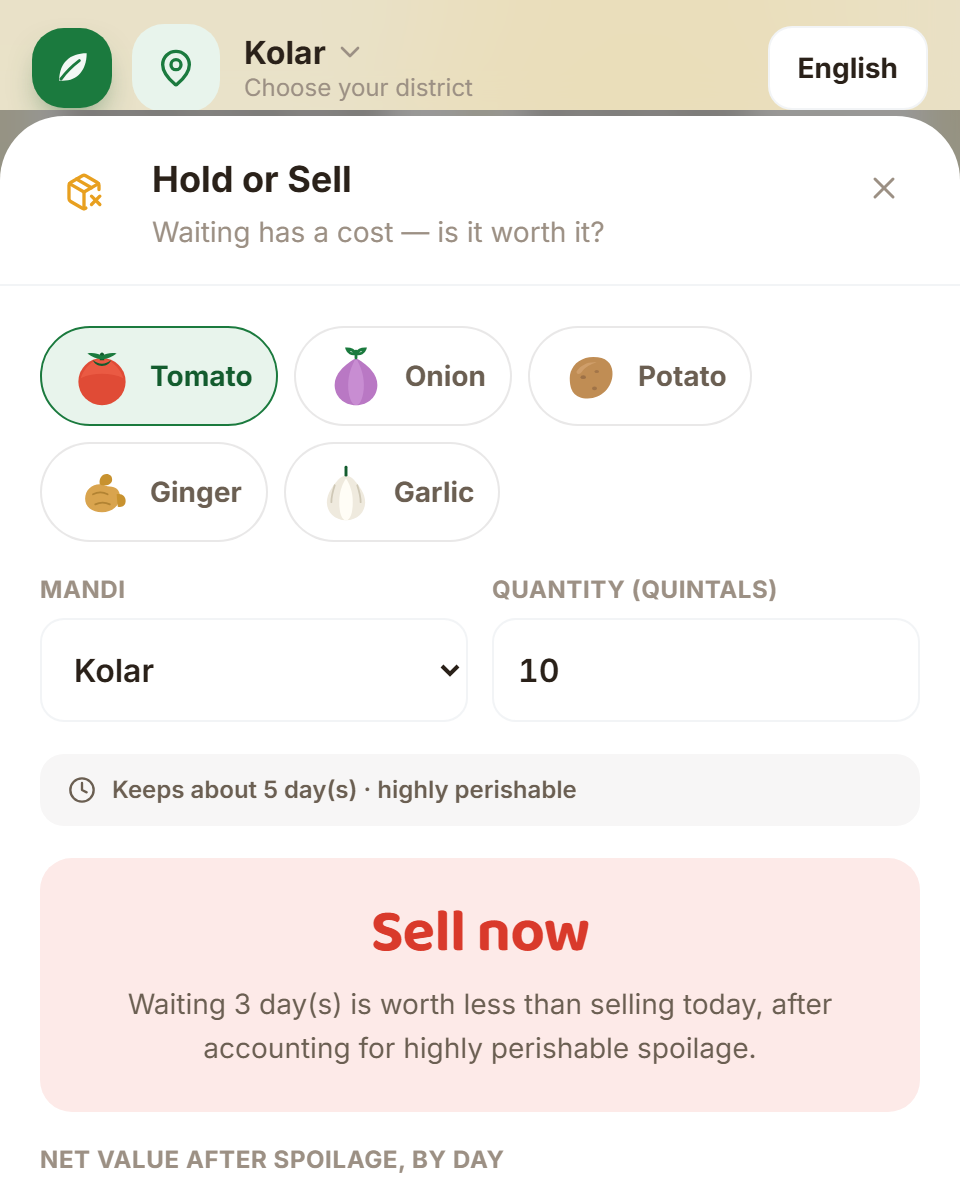
\includegraphics[width=0.94\linewidth,height=9.0cm,keepaspectratio]{figures/shot_t_holdorsell.png}}\\[1mm]{\footnotesize (a) Hold or sell}\end{minipage}\hfill
\begin{minipage}[t]{0.485\textwidth}\centering\fbox{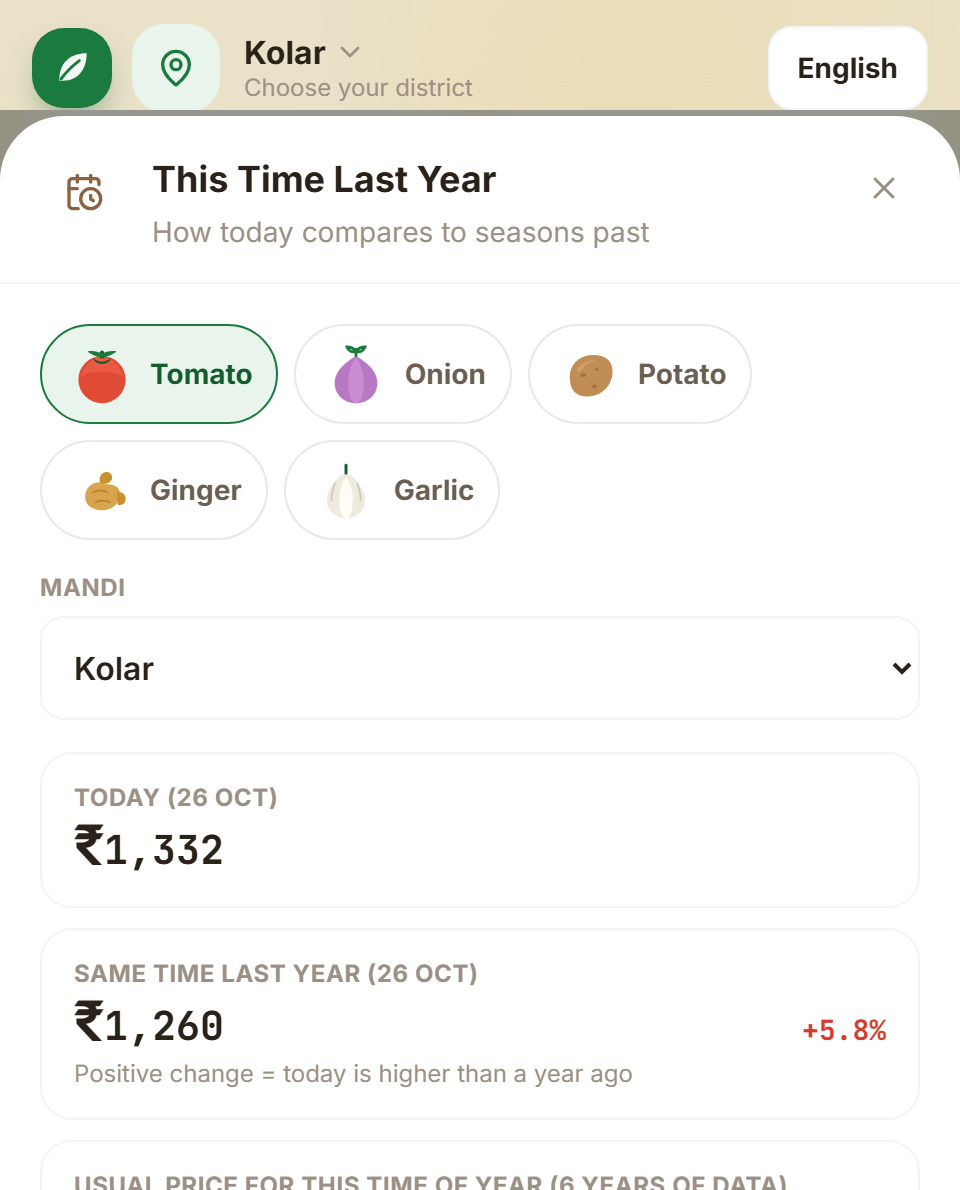
\includegraphics[width=0.94\linewidth,height=9.0cm,keepaspectratio]{figures/shot_t_lastyear.png}}\\[1mm]{\footnotesize (b) This time last year}\end{minipage}
\medskip
\centering \begin{minipage}[t]{0.485\textwidth}\centering\fbox{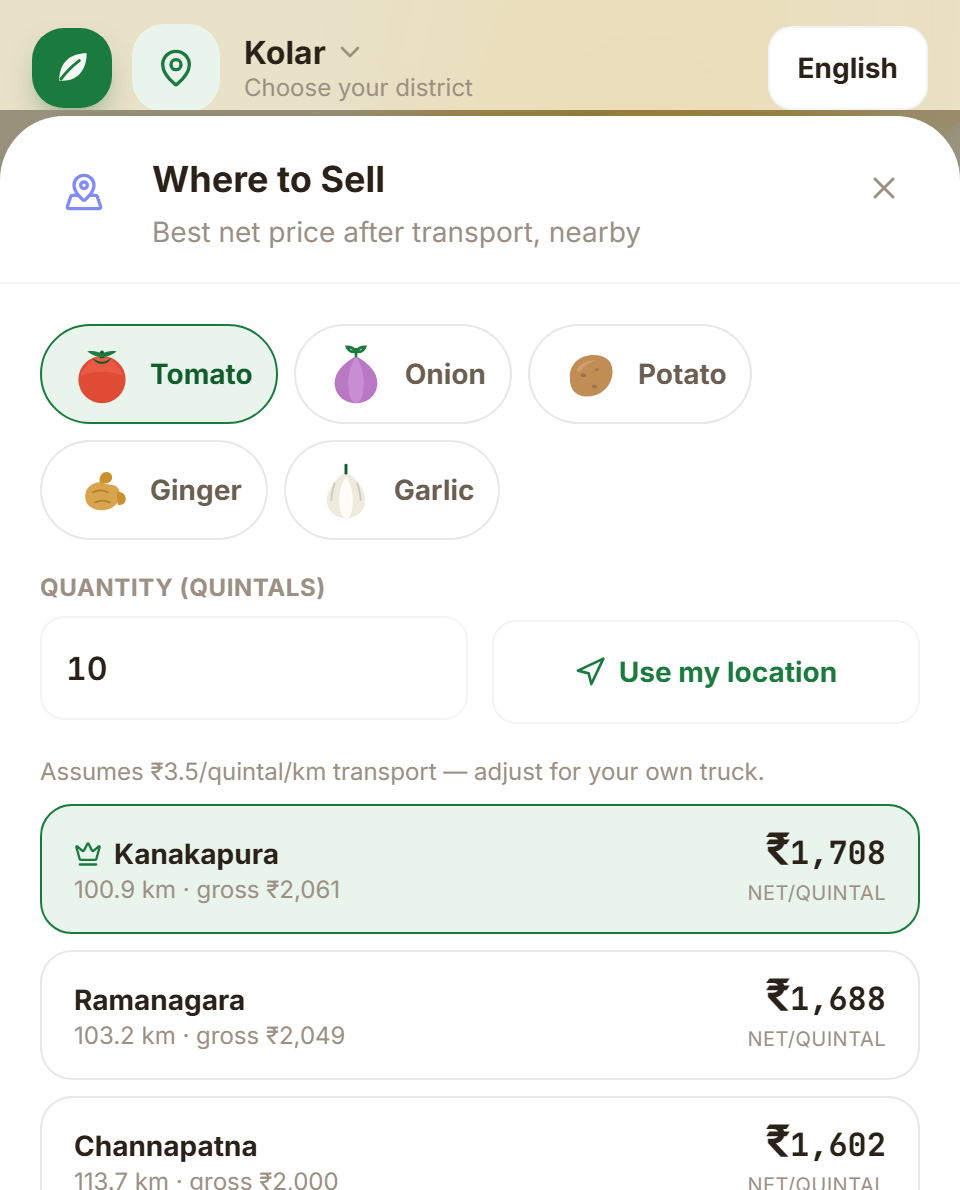
\includegraphics[width=0.94\linewidth,height=9.0cm,keepaspectratio]{figures/shot_t_wheretosell.png}}\\[1mm]{\footnotesize (c) Where to sell}\end{minipage}
\caption{Timing and location tools. (a) A hold-or-sell call that weighs spoilage against the expected price gain. (b) Today's price against the same date last year and the seasonal norm. (c) Nearby markets ranked by price after transport.}
\label{fig:sc-tools2}
\end{figure}

Hold or Sell (Figure~\ref{fig:sc-tools2}a) is built for the perishable case: it states the cost of waiting a day, so that ``wait'' is never the free option it appears to be. The seasonal sheet (b) gives context, not a forecast, and is labelled so. The ranking (c) lists markets with distance, gross price and net price per quintal under an assumed transport cost that the farmer can change.


\begin{figure}[!t]
\centering
\begin{minipage}[t]{0.485\textwidth}\centering\fbox{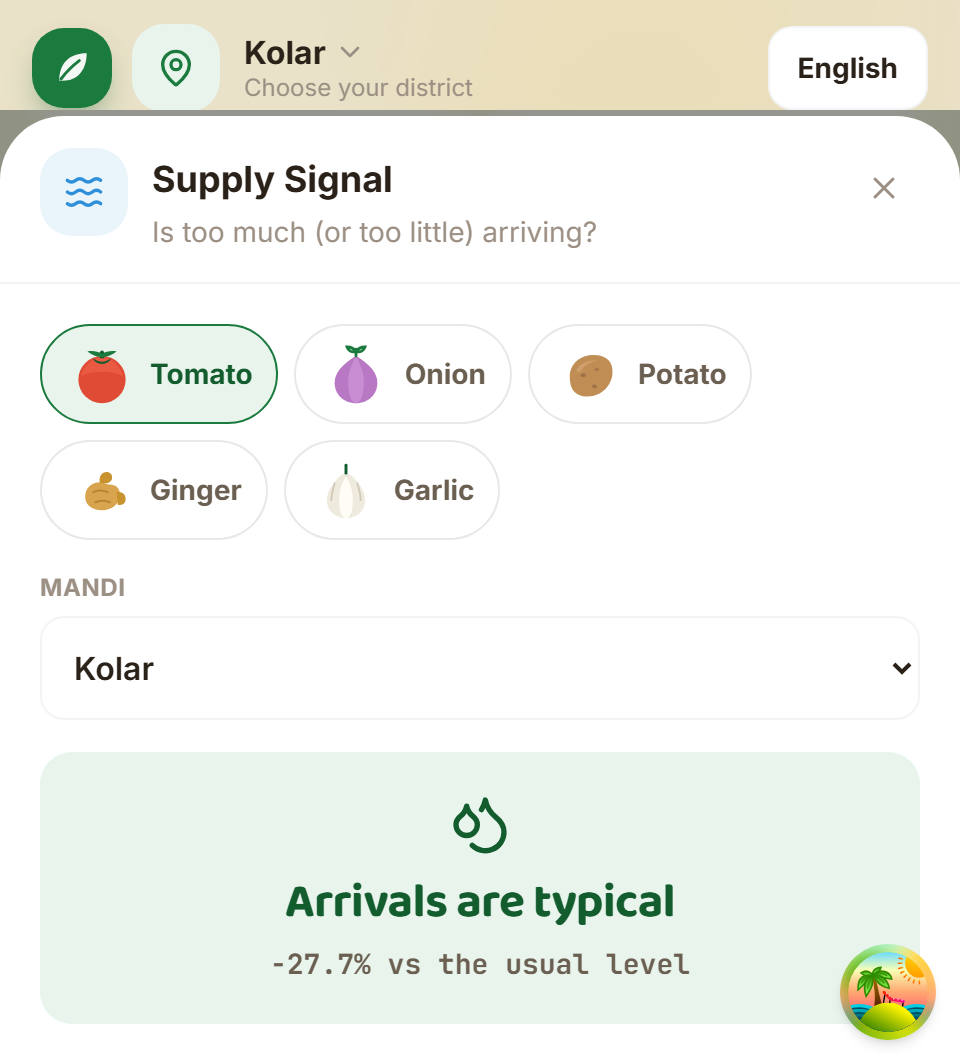
\includegraphics[width=0.94\linewidth,height=9.0cm,keepaspectratio]{figures/shot_t_supply.png}}\\[1mm]{\footnotesize (a) Supply signal}\end{minipage}\hfill
\begin{minipage}[t]{0.485\textwidth}\centering\fbox{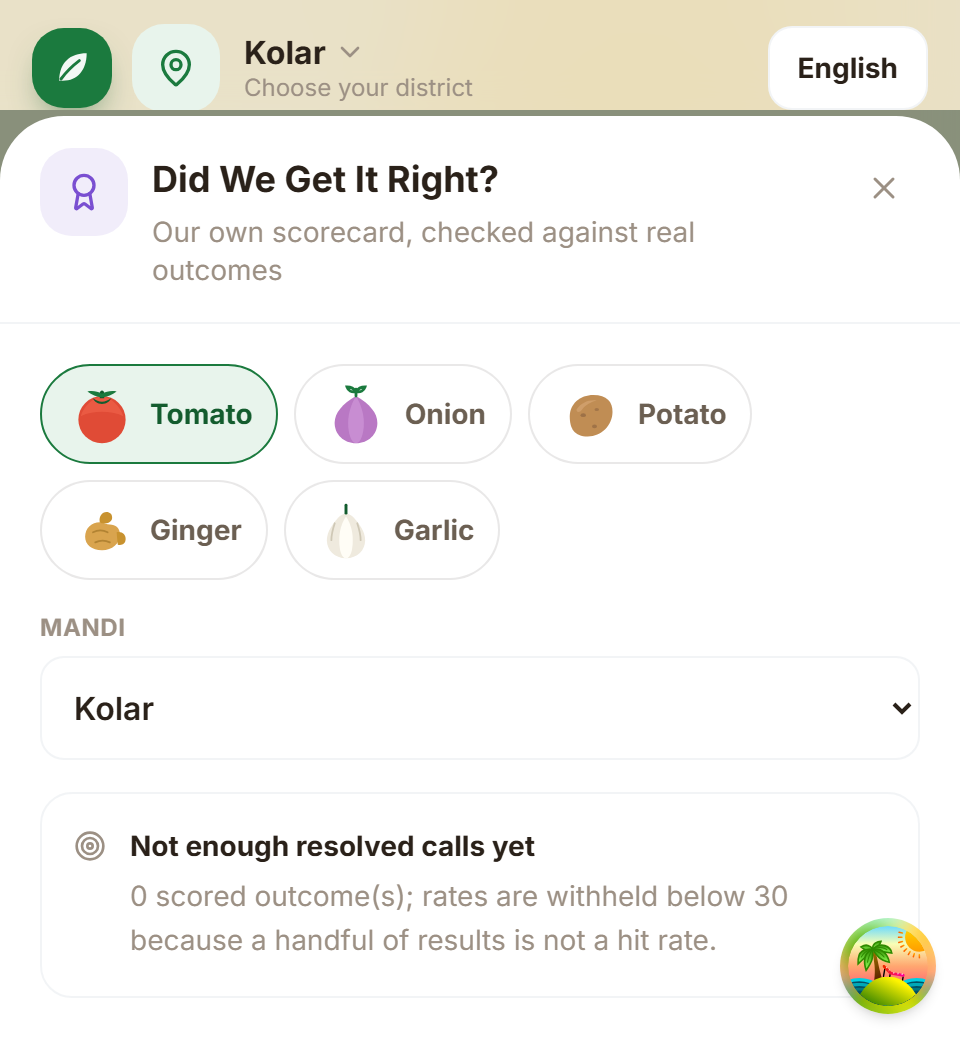
\includegraphics[width=0.94\linewidth,height=9.0cm,keepaspectratio]{figures/shot_t_record.png}}\\[1mm]{\footnotesize (b) Did we get it right?}\end{minipage}
\medskip
\centering \begin{minipage}[t]{0.485\textwidth}\centering\fbox{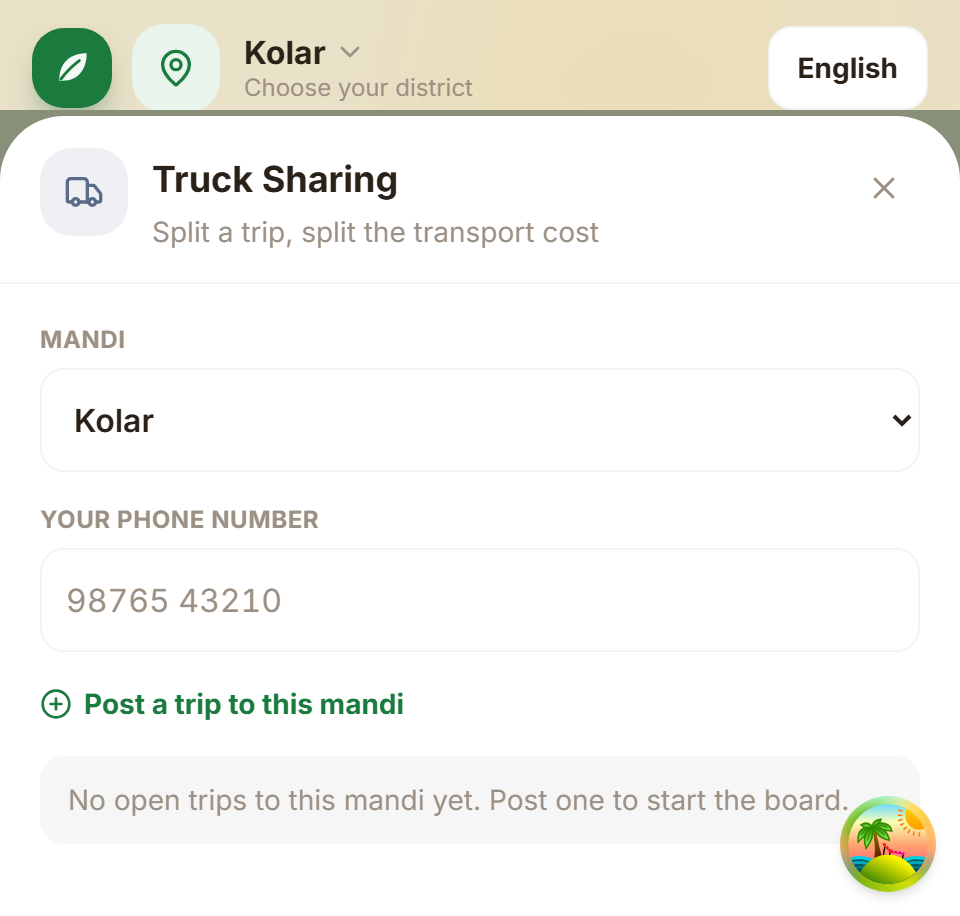
\includegraphics[width=0.94\linewidth,height=9.0cm,keepaspectratio]{figures/shot_t_truck.png}}\\[1mm]{\footnotesize (c) Truck sharing}\end{minipage}
\caption{Context and sharing tools. (a) Arrivals against the usual level. (b) The system's own scorecard of resolved calls. (c) A board for splitting a truck to a market.}
\label{fig:sc-tools3}
\end{figure}

The supply signal (Figure~\ref{fig:sc-tools3}a) reports whether arrivals are unusually high or low, since a glut lowers price. The scorecard (b) is an honest counter: when too few calls have resolved it says so and withholds the rate. The truck-sharing board (c) is a prototype that lets a farmer post a trip so that others can share the transport cost.


\begin{figure}[!t]
\centering
\begin{minipage}[t]{0.485\textwidth}\centering\fbox{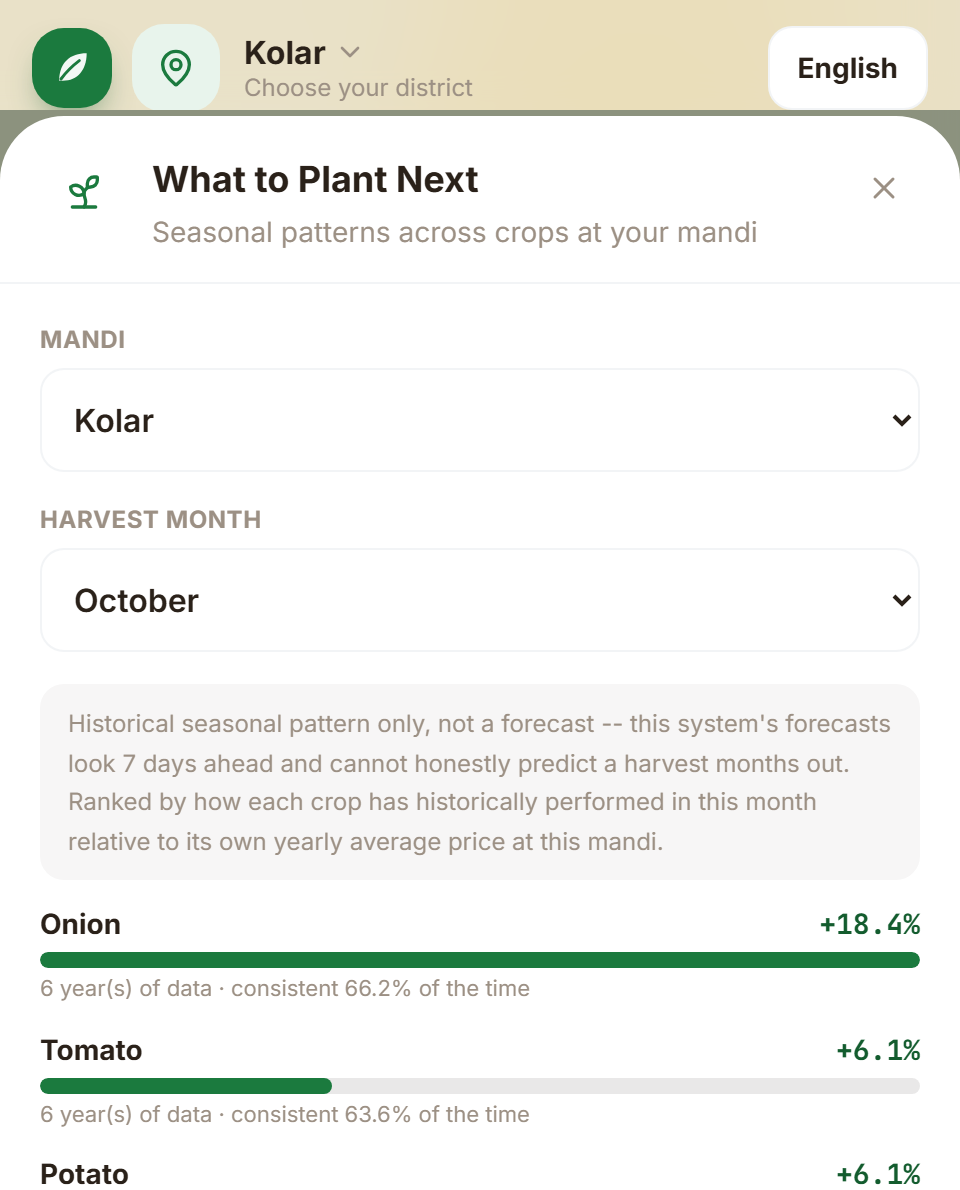
\includegraphics[width=0.94\linewidth,height=9.0cm,keepaspectratio]{figures/shot_t_plant.png}}\\[1mm]{\footnotesize (a) What to plant next}\end{minipage}\hfill
\begin{minipage}[t]{0.485\textwidth}\centering\fbox{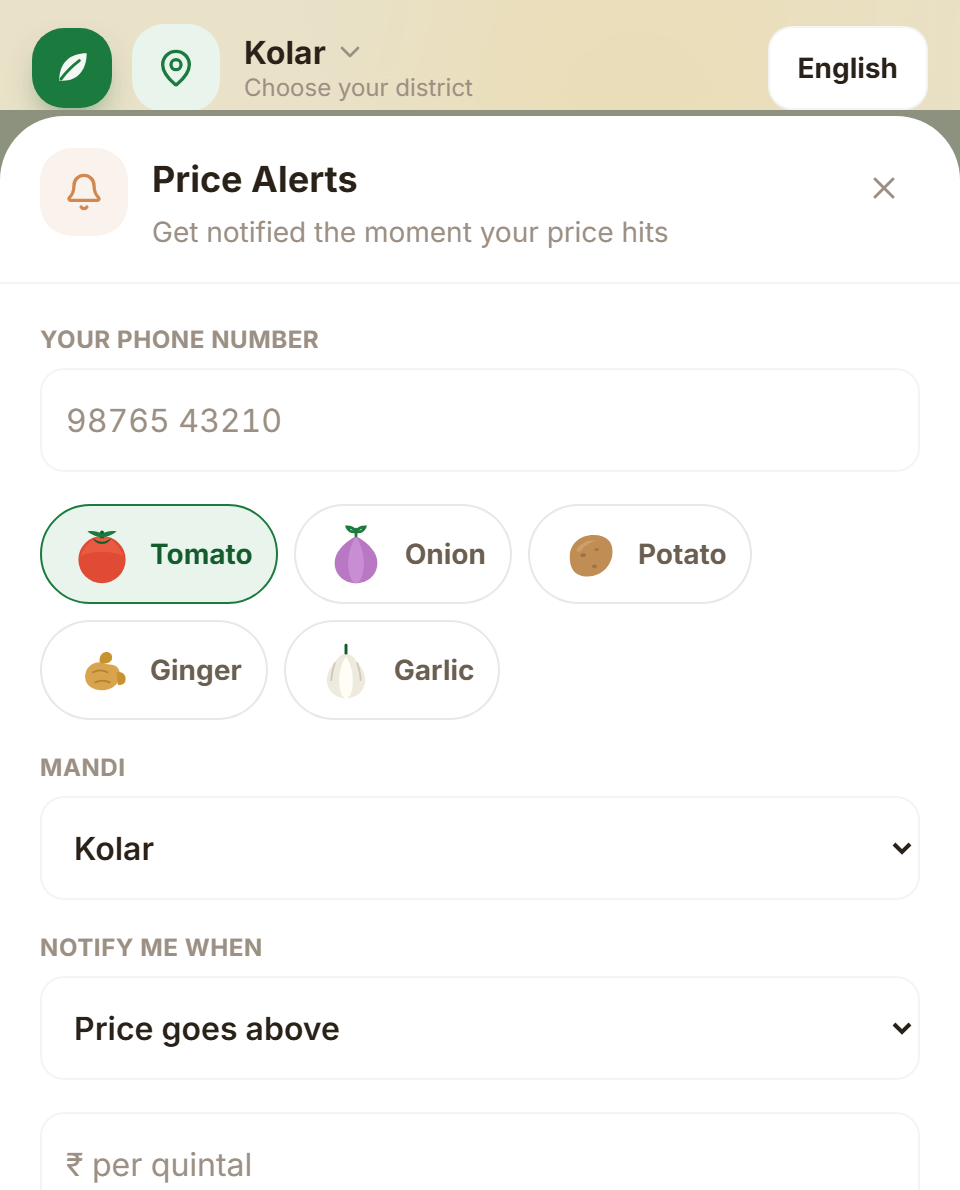
\includegraphics[width=0.94\linewidth,height=9.0cm,keepaspectratio]{figures/shot_t_alerts.png}}\\[1mm]{\footnotesize (b) Price alerts}\end{minipage}
\caption{(a) Seasonal patterns by crop for a chosen harvest month, from past years. (b) A price alert that notifies the farmer when a crop reaches a chosen price.}
\label{fig:sc-tools4}
\end{figure}

What to Plant Next (Figure~\ref{fig:sc-tools4}a) is explicitly historical: it shows how each crop has behaved in the chosen month in previous years and does not forecast the coming season. The alert sheet (b) is the entry point for the Telegram digest of Section~\ref{sec:digest-method}.


\subsection{Advice that can be checked}
The three panels of Figure~\ref{fig:ui-insight} (Section~\ref{sec:insight-method}) sit inside the Best Place sheet. They show the arithmetic behind the choice, what changes if the farmer's costs differ, and how the advice would have done on days it had not seen. The morning digest of Section~\ref{sec:digest-method} is the same advice delivered as a message.

\subsection{Trader desk}
The trader desk is a set of analytical tools for buyers and for the project's own examination of its method. It is laid out for a wide screen.

\begin{figure}[!t]
\centering
\fbox{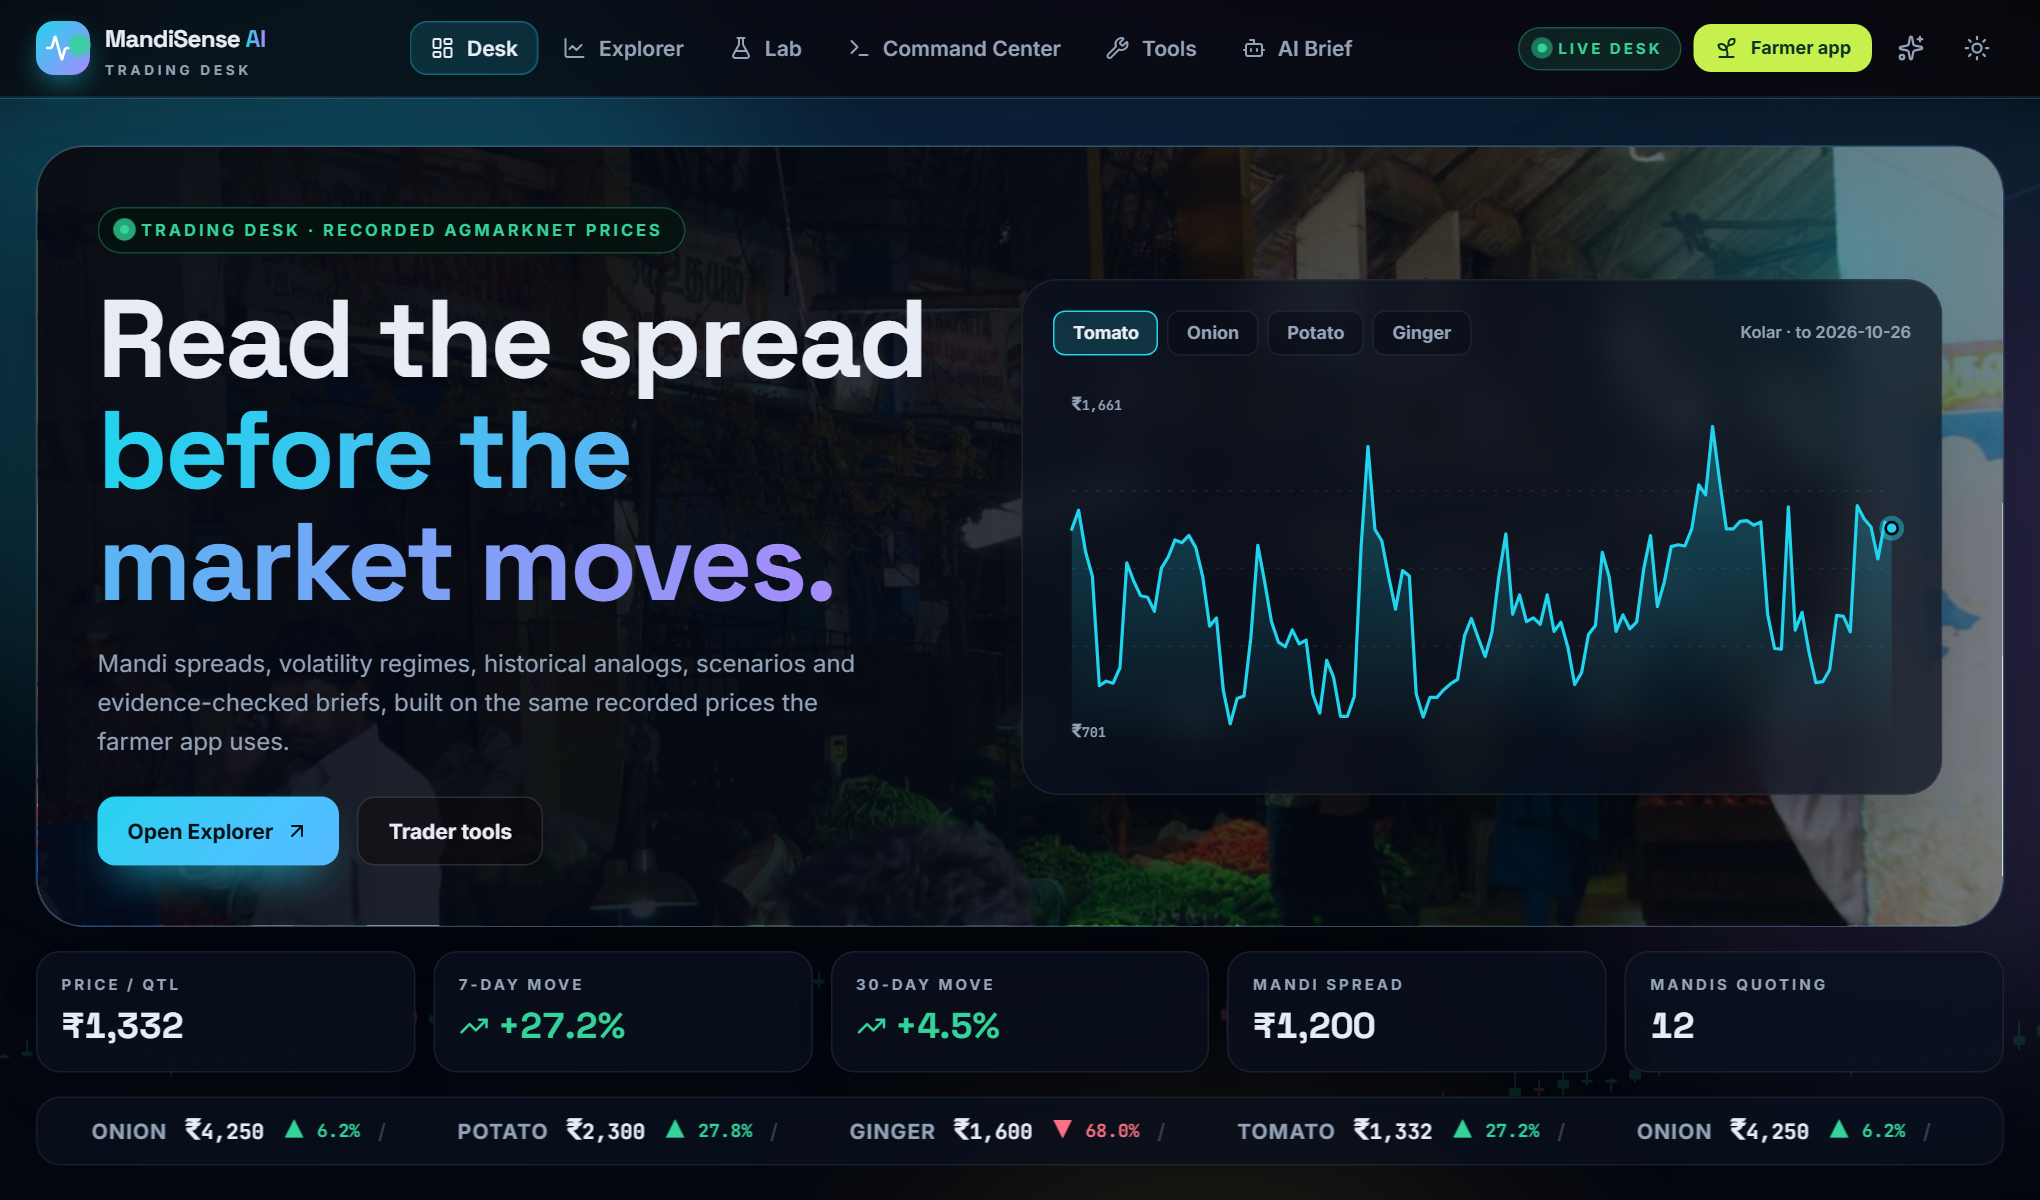
\includegraphics[width=0.93\linewidth]{figures/shot_w_trader.png}}\\[0.5mm]{\footnotesize (a) Trader home: the day's key signals and entry points to the tools below}
\medskip
\fbox{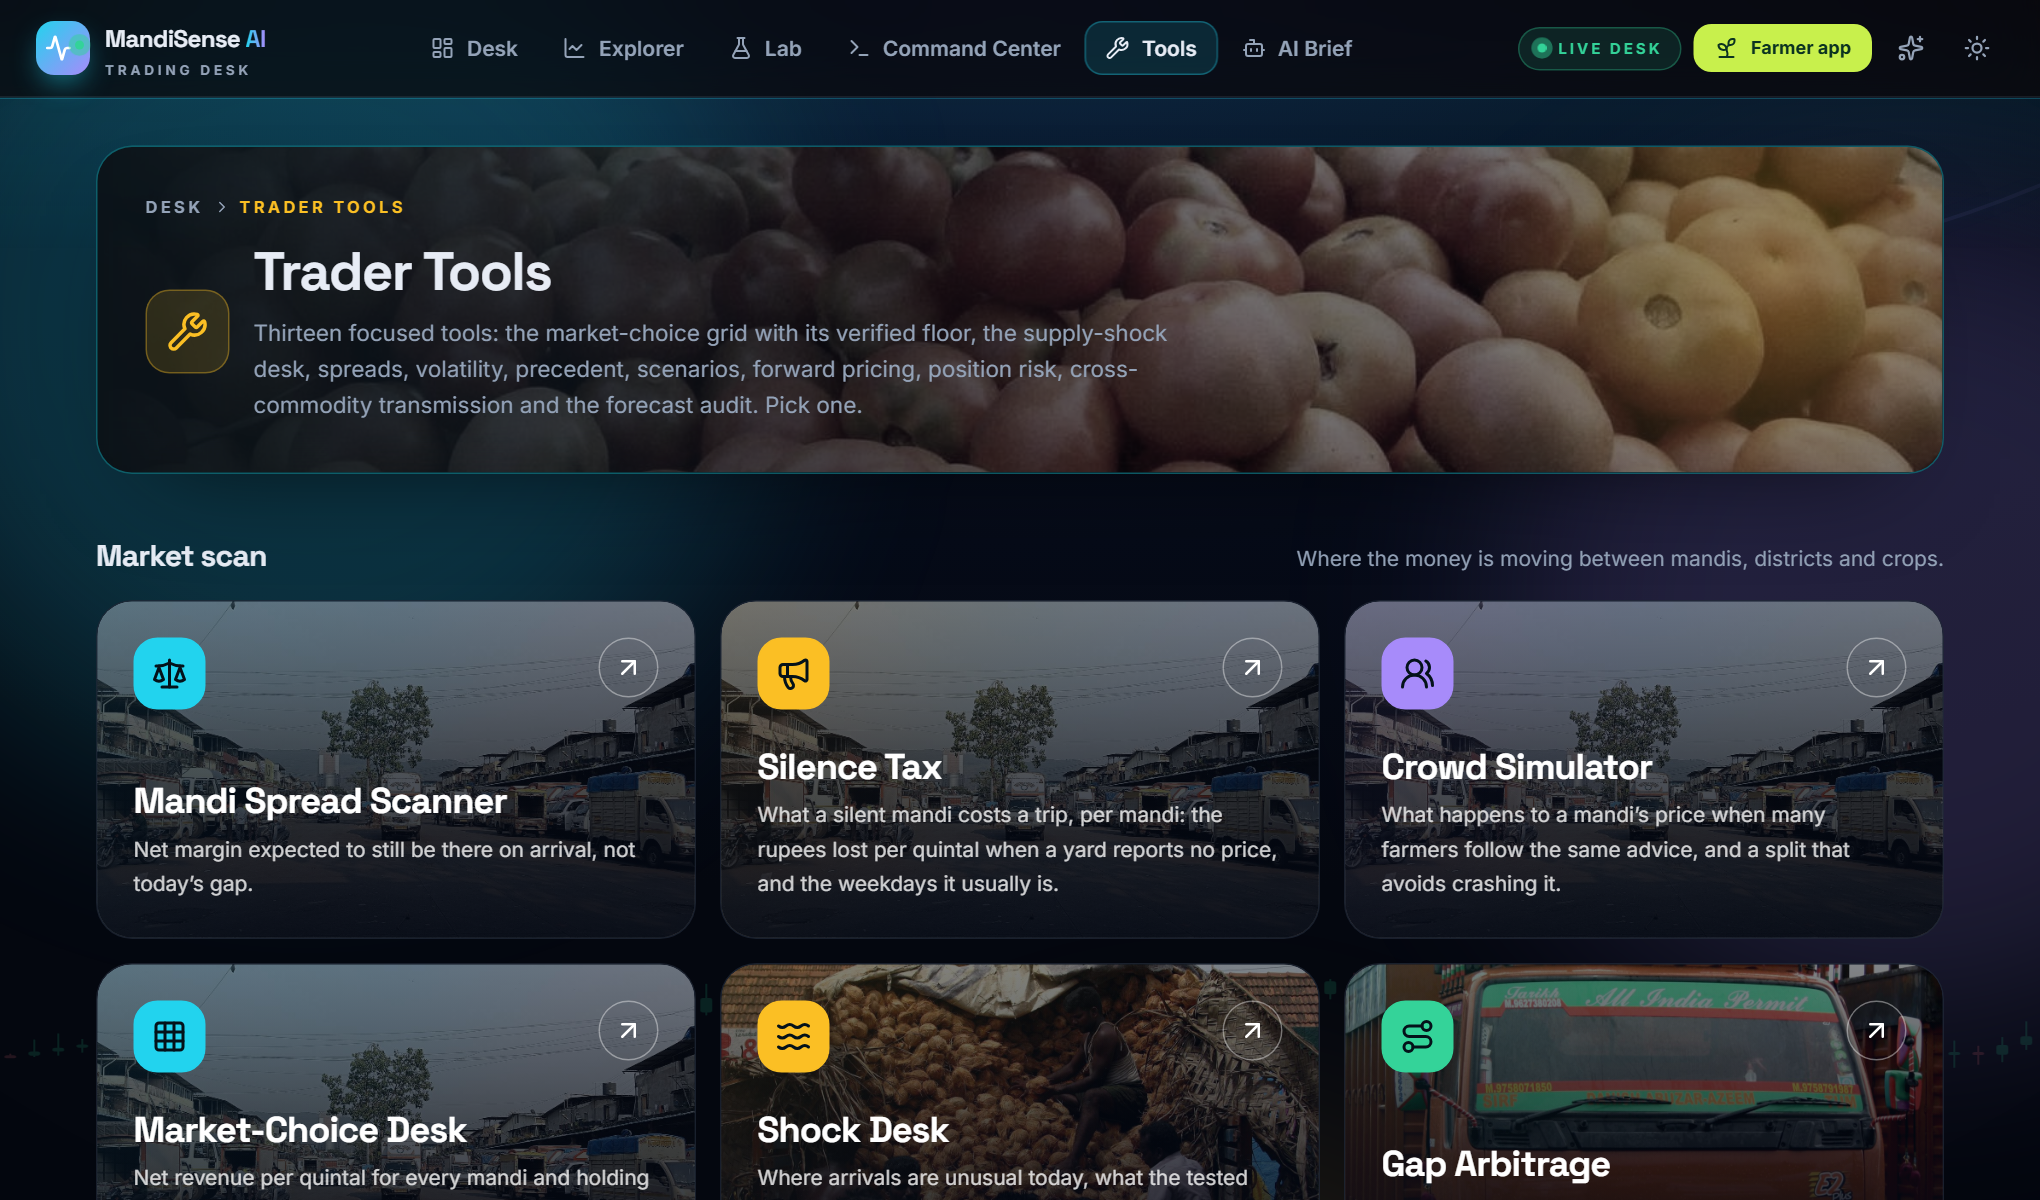
\includegraphics[width=0.93\linewidth]{figures/shot_w_tradertools.png}}\\[0.5mm]{\footnotesize (b) The trader tools index}
\caption{(a) Trader home: the day's key signals and entry points to the tools below. (b) The trader tools index.}
\label{fig:sc-w-trader}
\end{figure}

The trader home page gathers the day's signals, such as the largest price gaps between markets, supply shocks and the status of the advice, and links each to its tool.

The index lists every analytical tool with a one-line statement of the question it answers.

\begin{figure}[!t]
\centering
\fbox{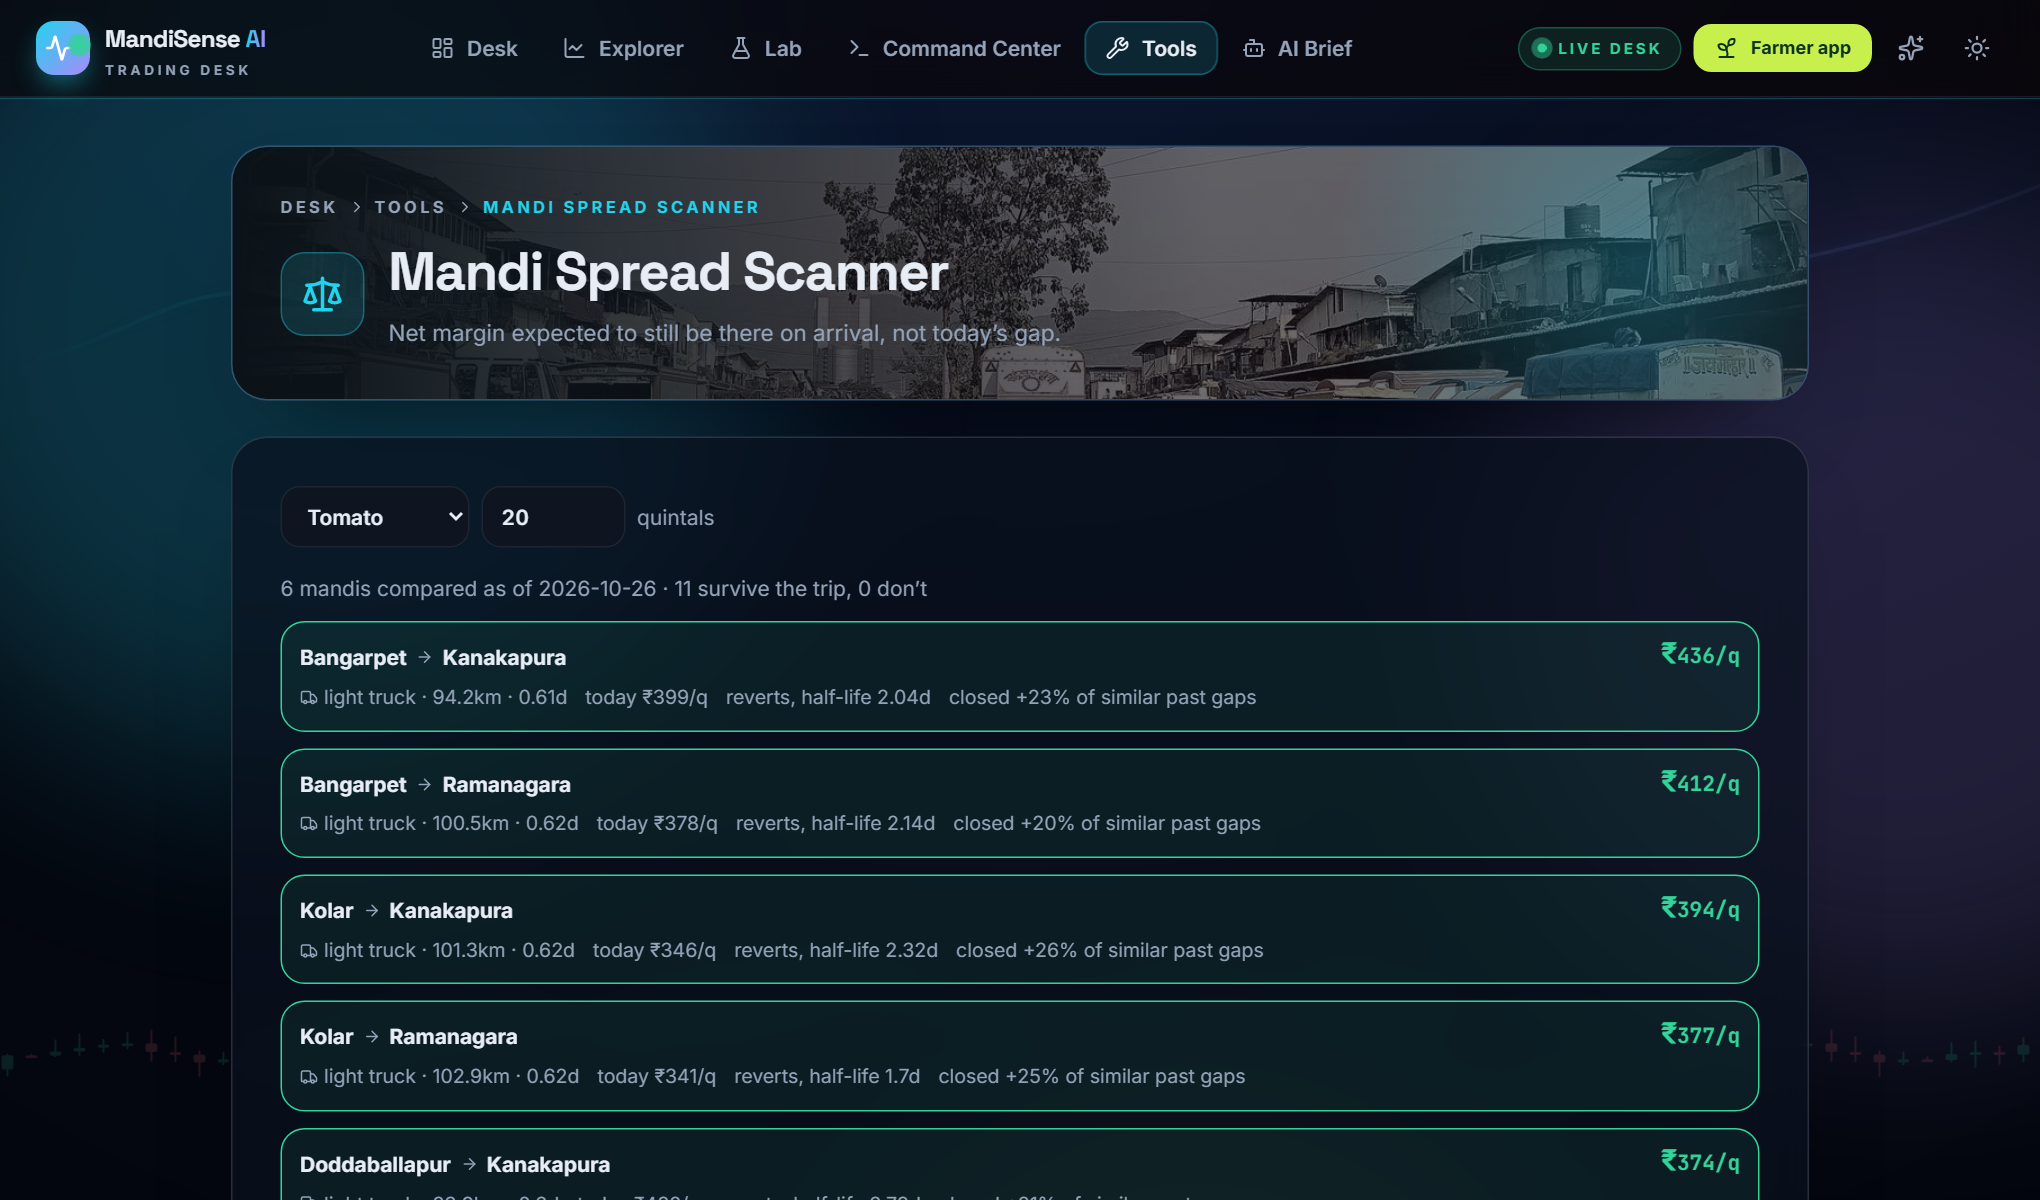
\includegraphics[width=0.93\linewidth]{figures/shot_w_spreads.png}}\\[0.5mm]{\footnotesize (a) Spreads between markets for one commodity}
\medskip
\fbox{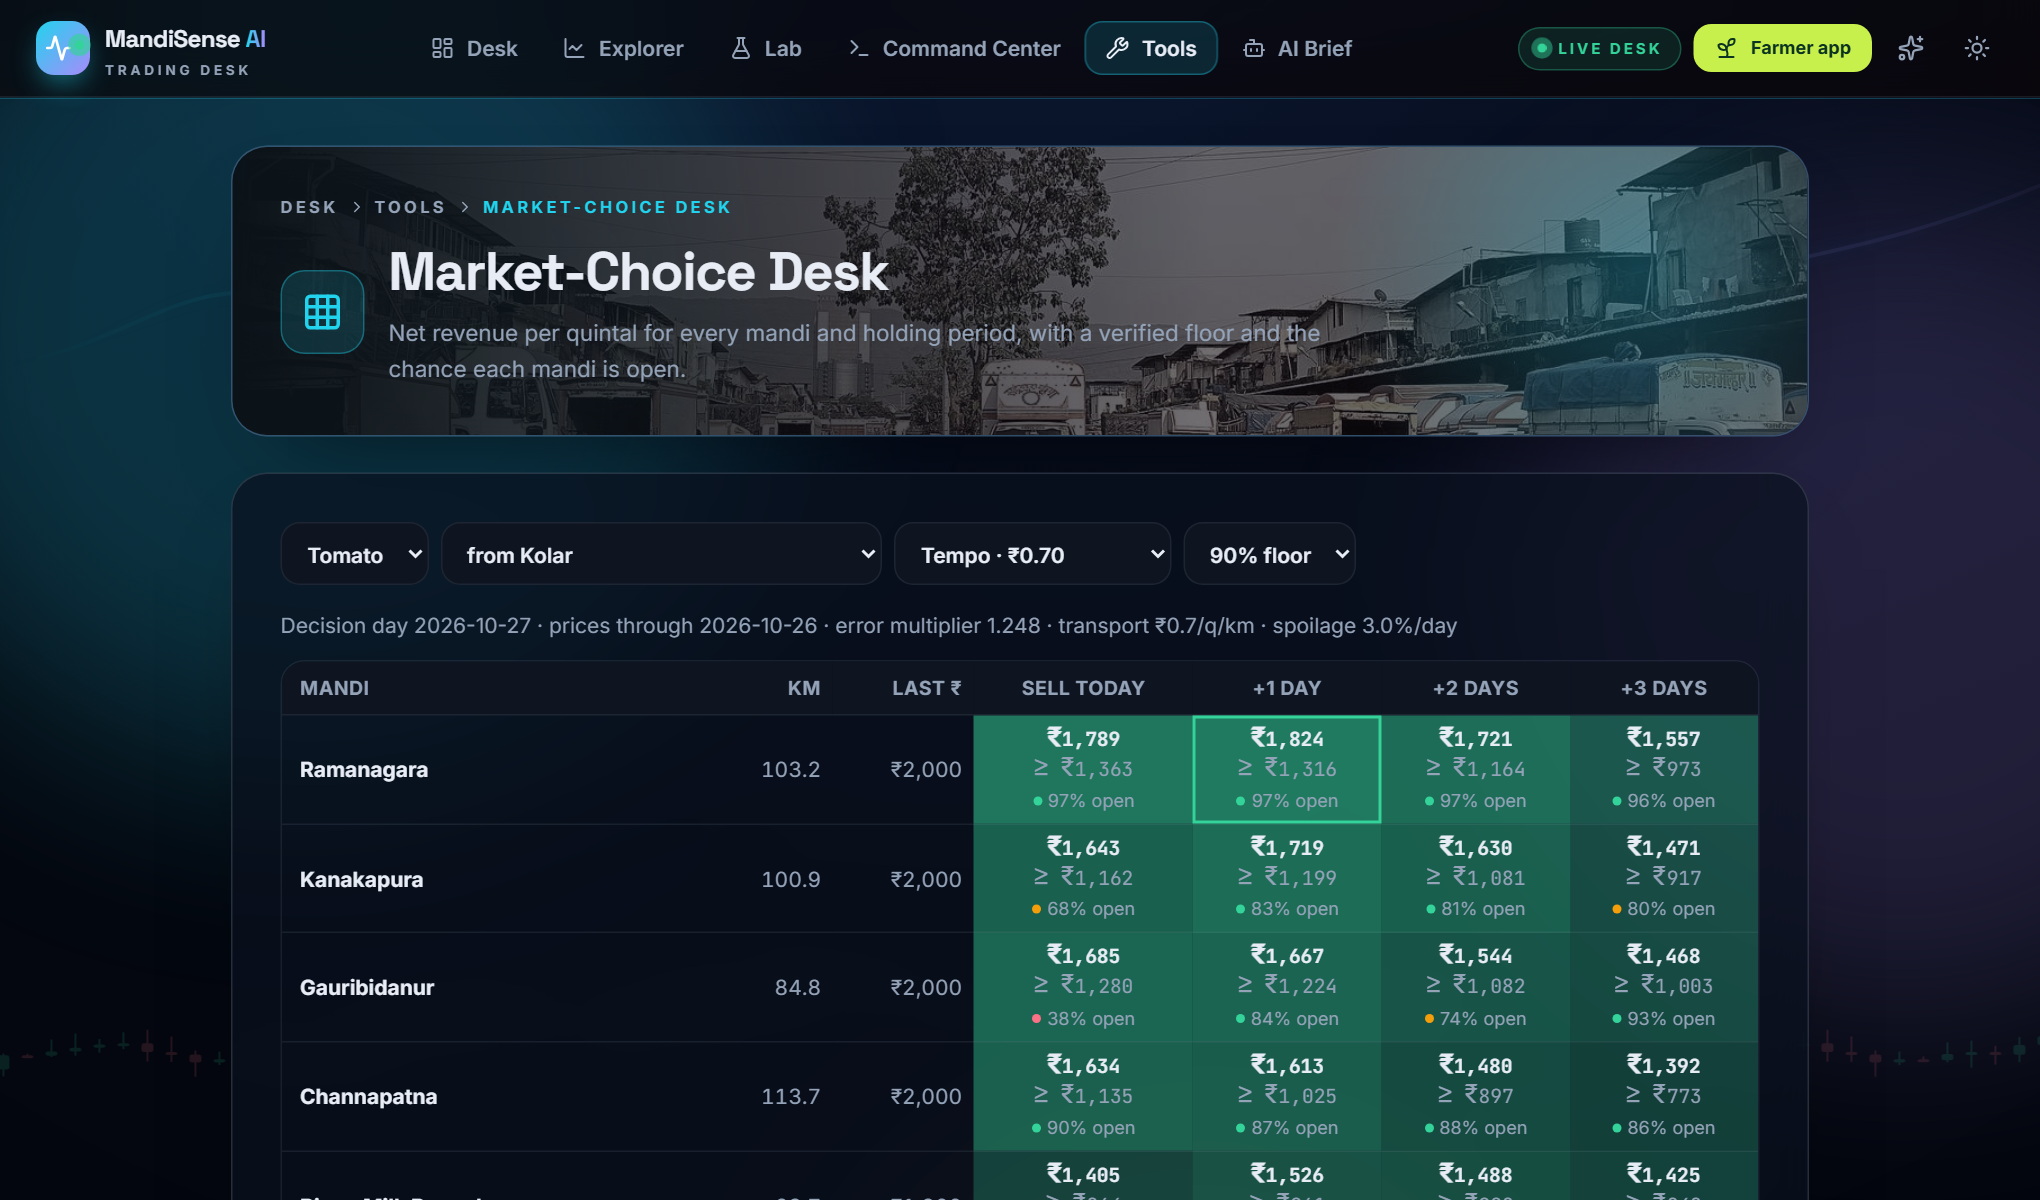
\includegraphics[width=0.93\linewidth]{figures/shot_w_mcdesk.png}}\\[0.5mm]{\footnotesize (b) The market-choice desk: the model's recommended market per day and the revenue floor}
\caption{(a) Spreads between markets for one commodity. (b) The market-choice desk: the model's recommended market per day and the revenue floor.}
\label{fig:sc-w-spreads}
\end{figure}

The spread tool shows the price gap between pairs of markets after transport, with the number of days each gap has lasted. A gap that persists is a signal of a market that is slow to clear.

This is the technical view of the recommendation of Section~\ref{sec:floors}: the chosen market, the expected and floor revenue, the alternatives and the model that produced them.

\begin{figure}[!t]
\centering
\fbox{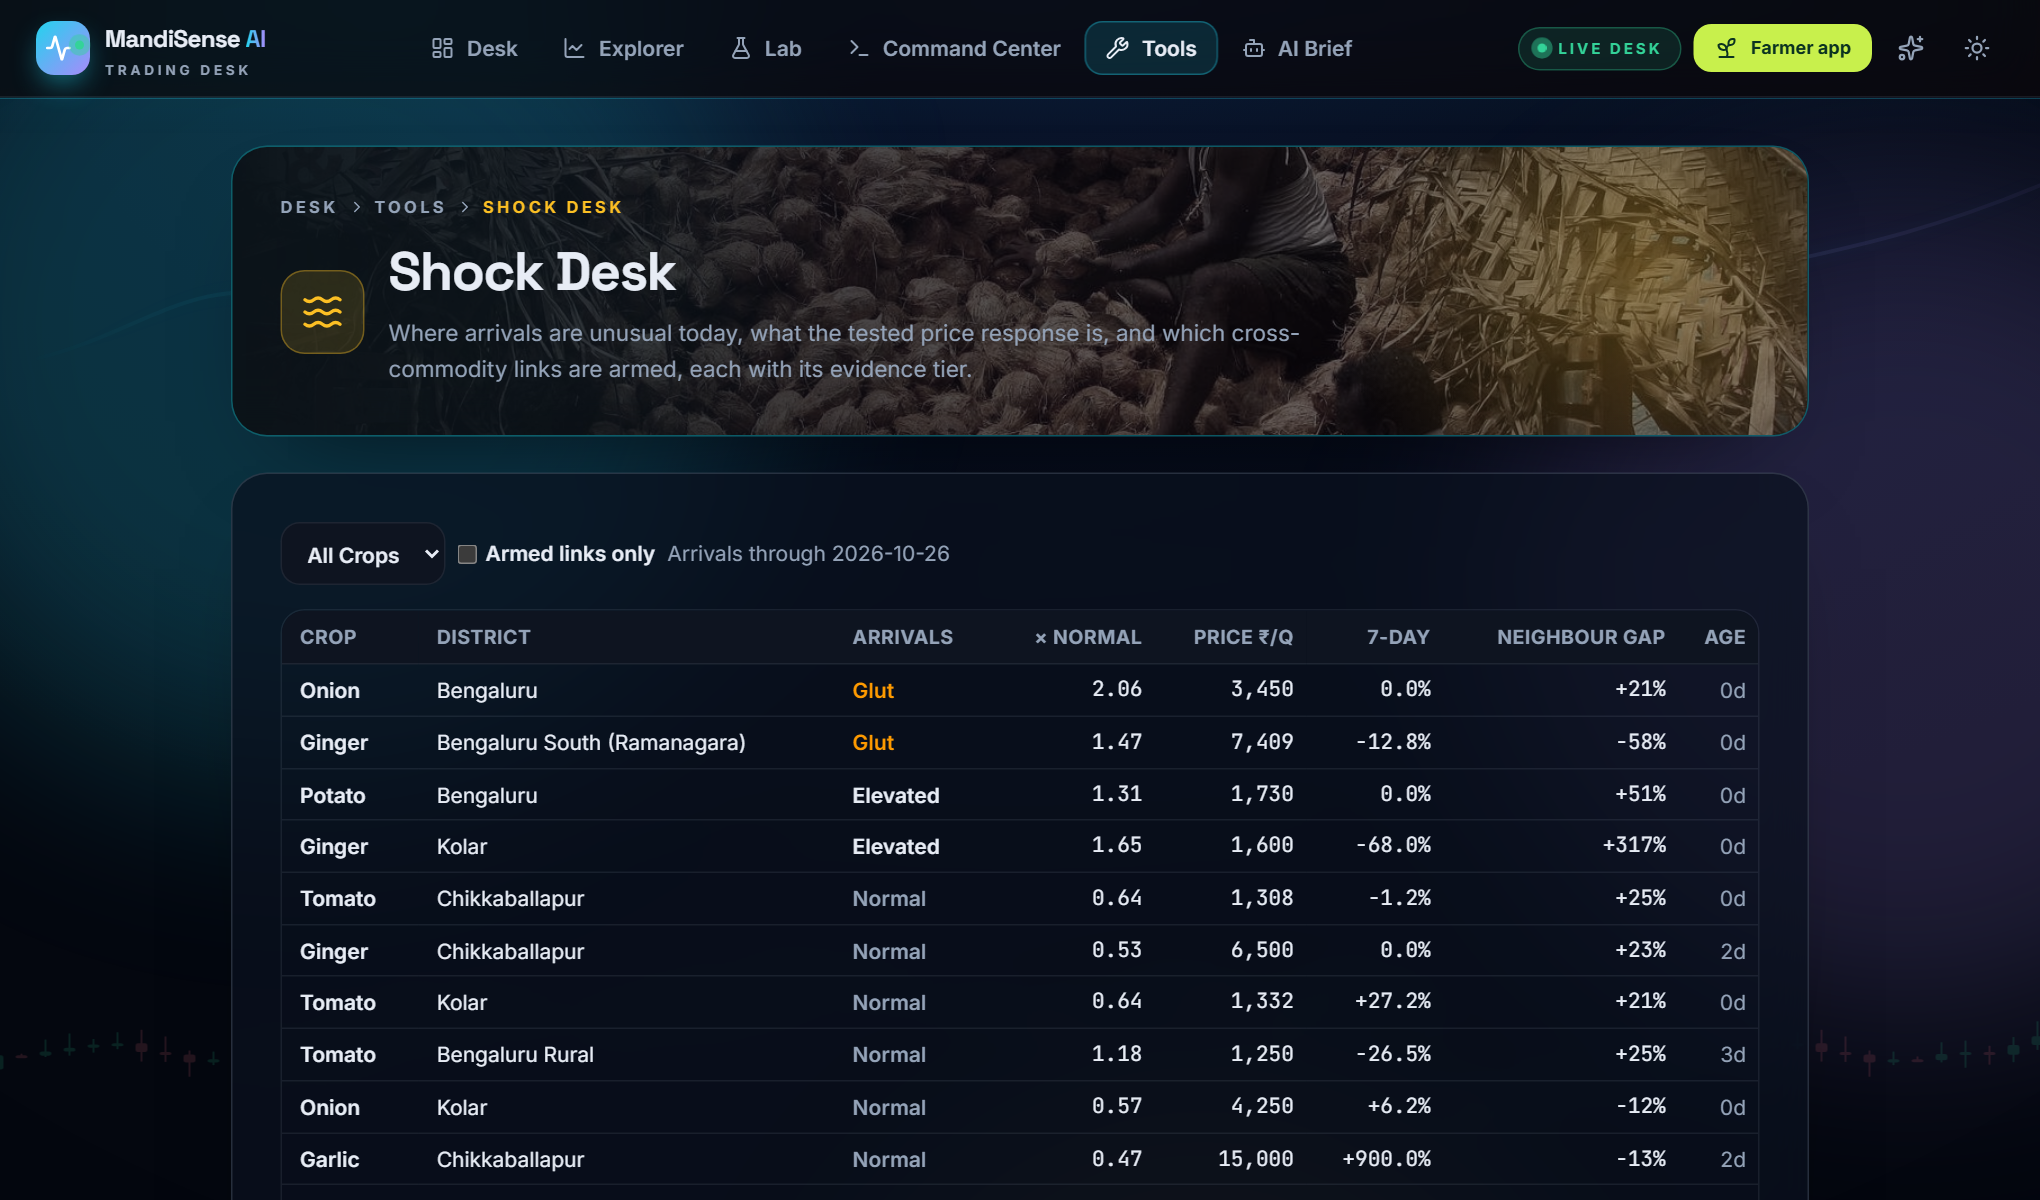
\includegraphics[width=0.93\linewidth]{figures/shot_w_shock.png}}\\[0.5mm]{\footnotesize (a) The shock desk: unusual price moves, with the markets affected}
\medskip
\fbox{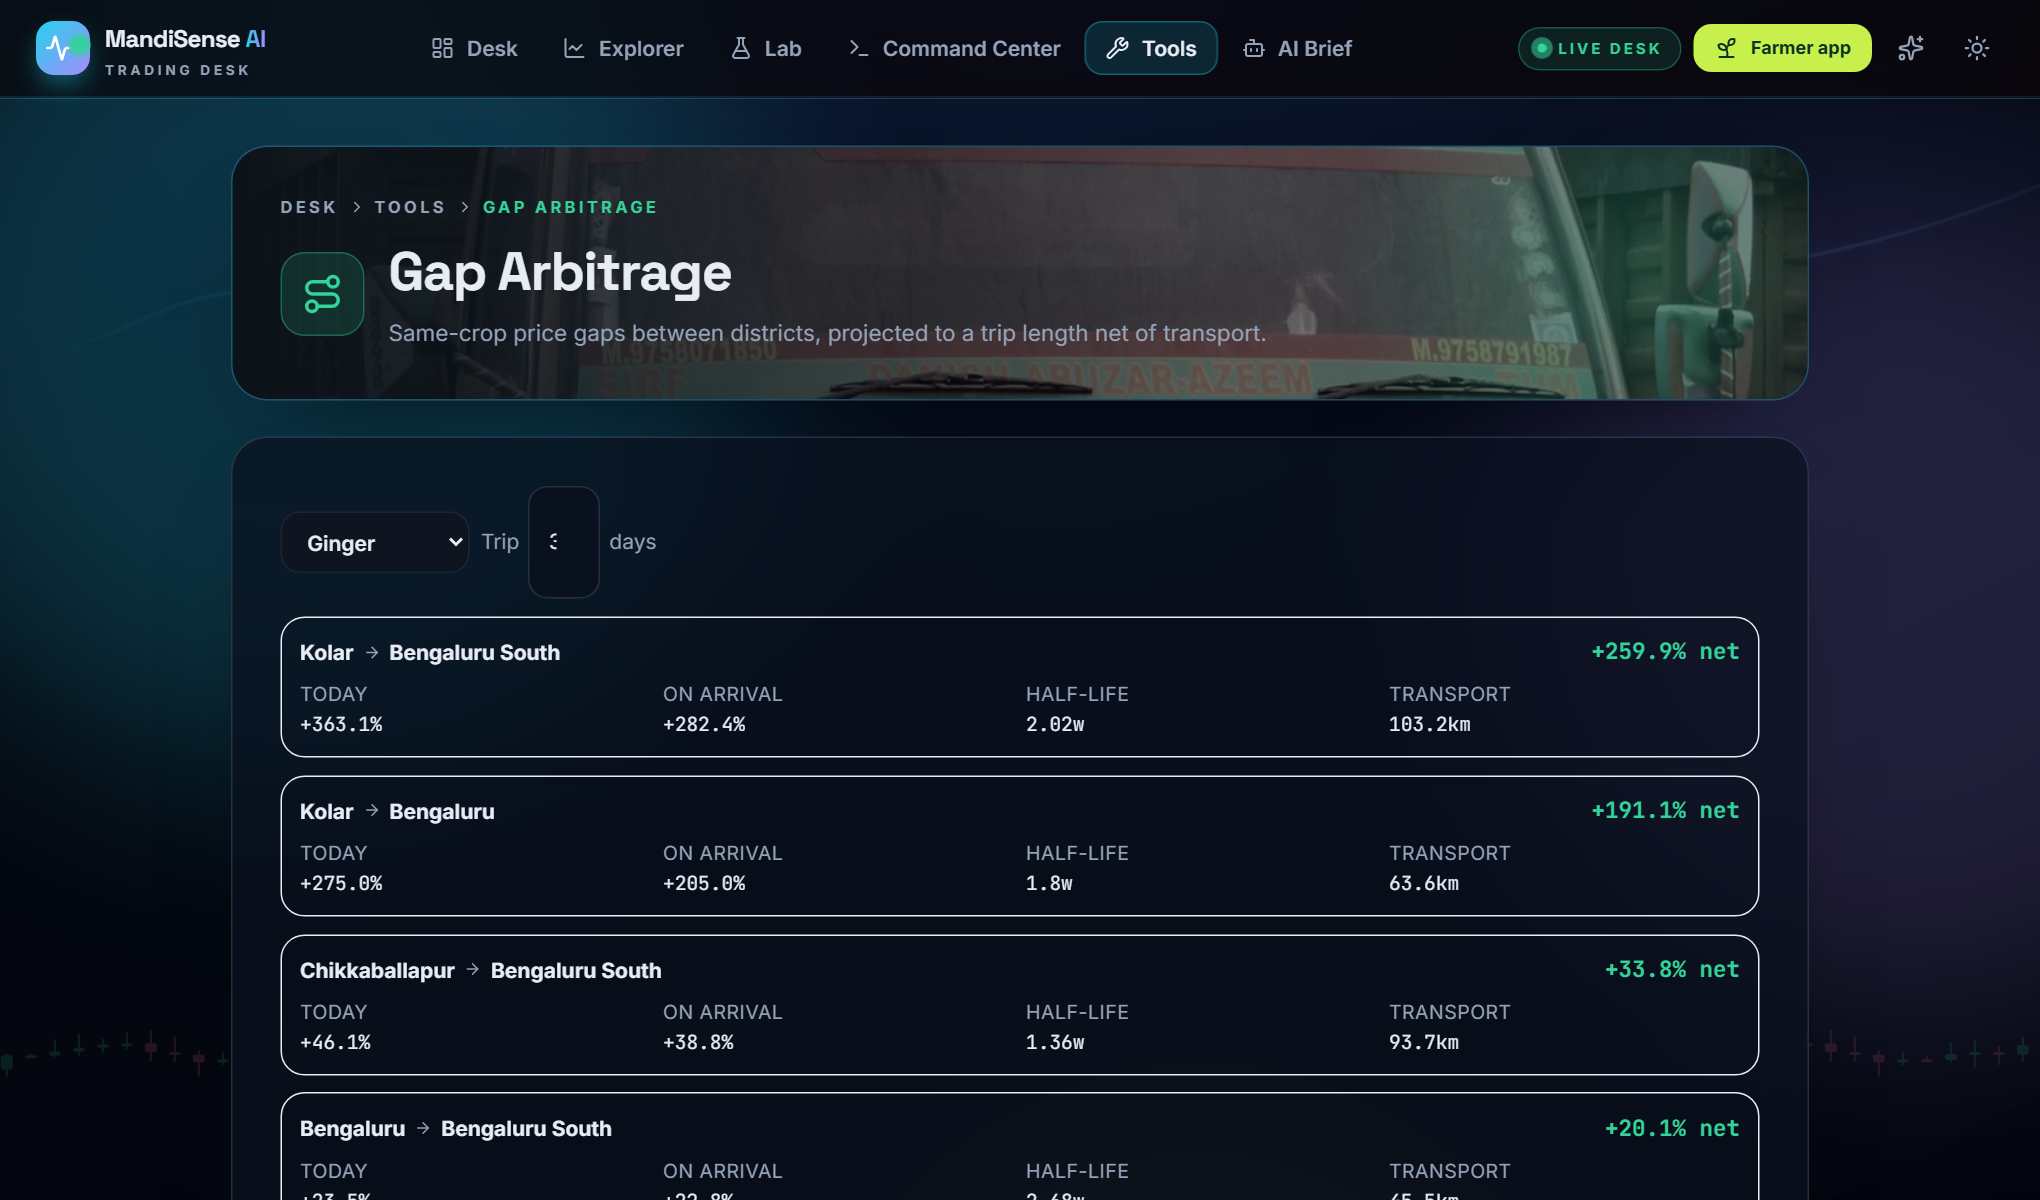
\includegraphics[width=0.93\linewidth]{figures/shot_w_gap.png}}\\[0.5mm]{\footnotesize (b) Gap arbitrage between mandis}
\caption{(a) The shock desk: unusual price moves, with the markets affected. (b) Gap arbitrage between mandis.}
\label{fig:sc-w-shock}
\end{figure}

The desk lists price moves that are unusual relative to a rolling baseline and the markets where they appear. It feeds the shock episodes used for the transmission test of Section~\ref{sec:spill-method}.

The tool pairs a high-price and a low-price market, deducts transport and shrinkage, and shows whether a gap is worth acting on.

\begin{figure}[!t]
\centering
\fbox{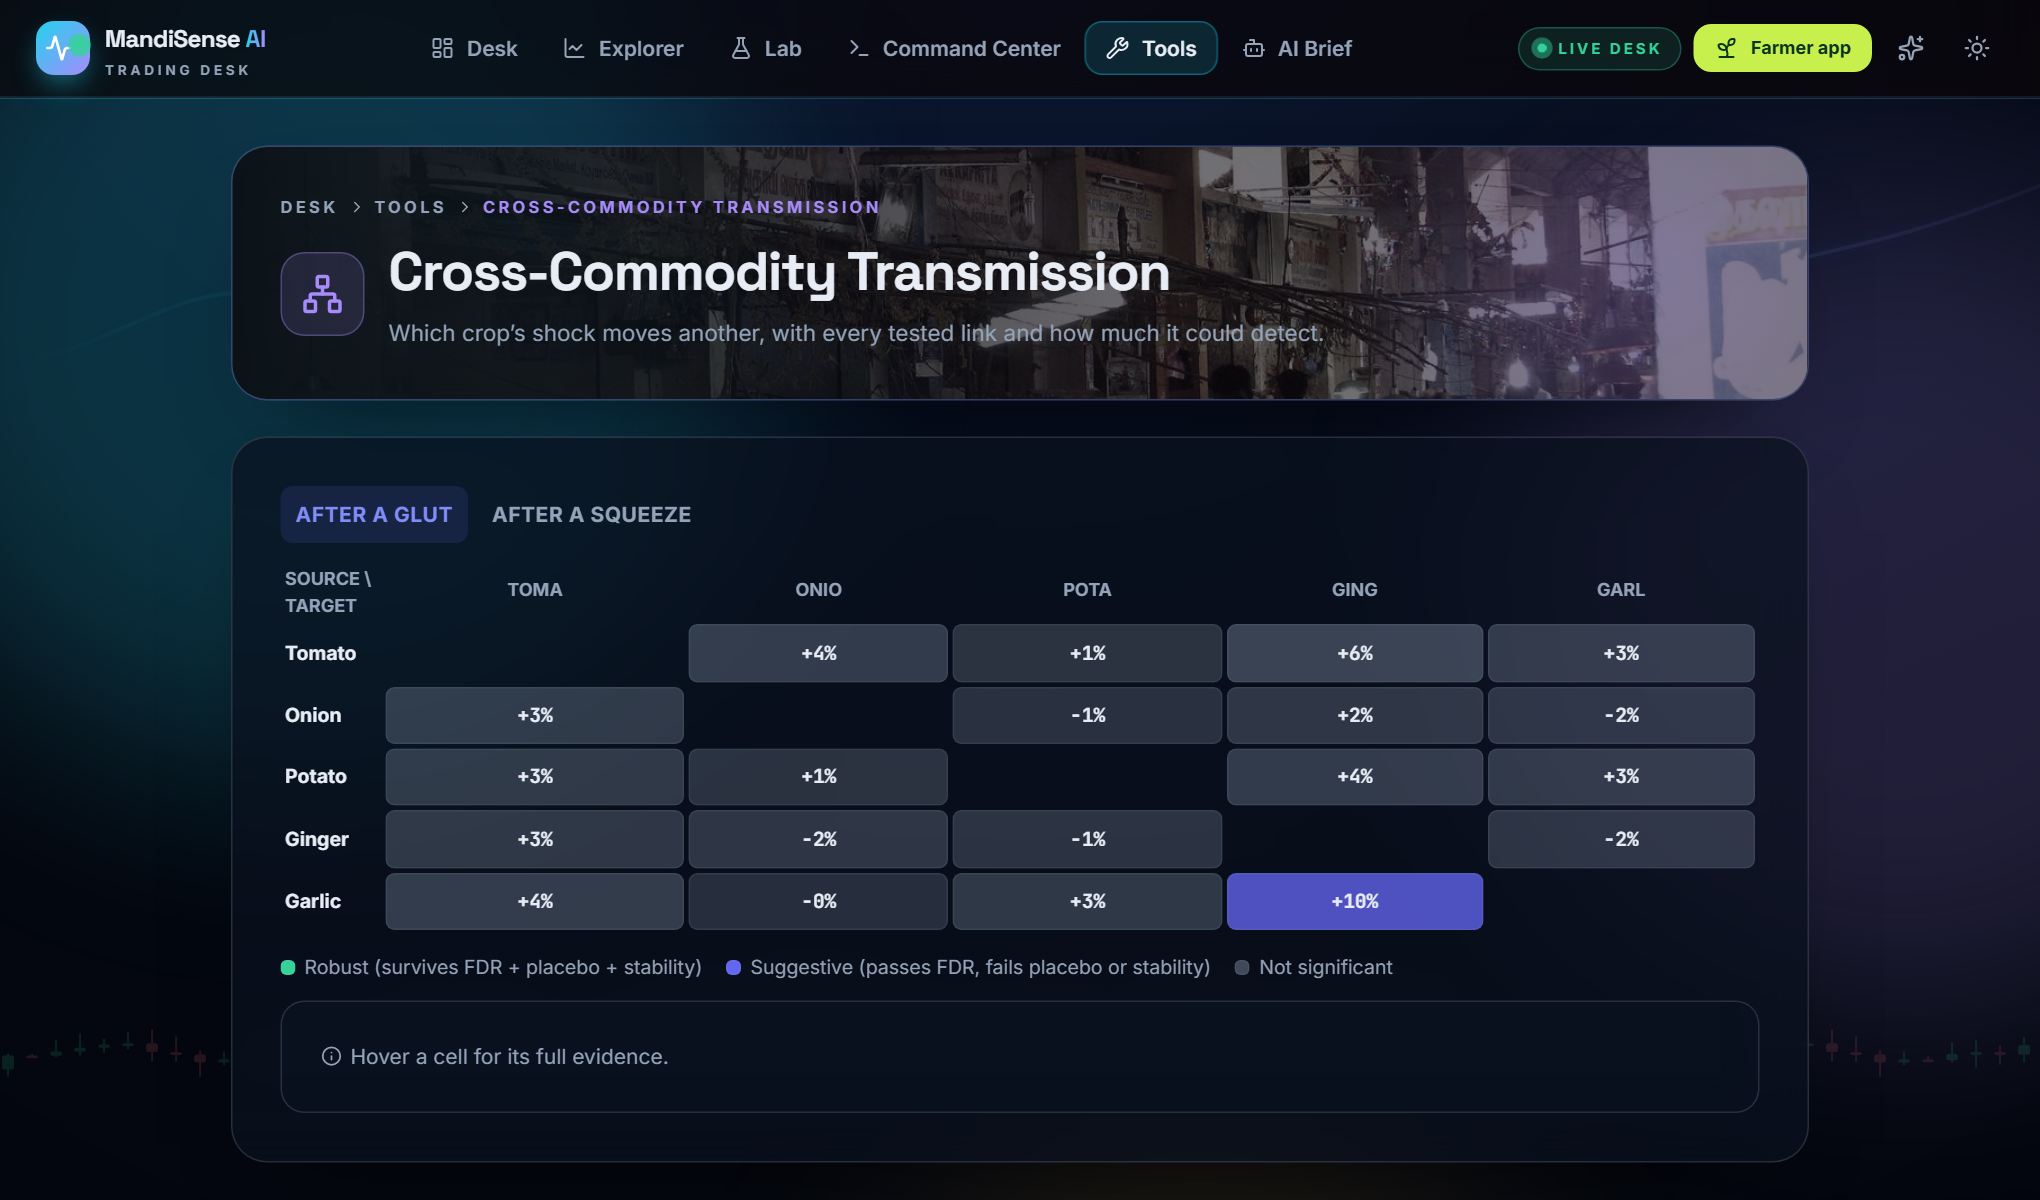
\includegraphics[width=0.93\linewidth]{figures/shot_w_transmission.png}}\\[0.5mm]{\footnotesize (a) Cross-commodity transmission}
\medskip
\fbox{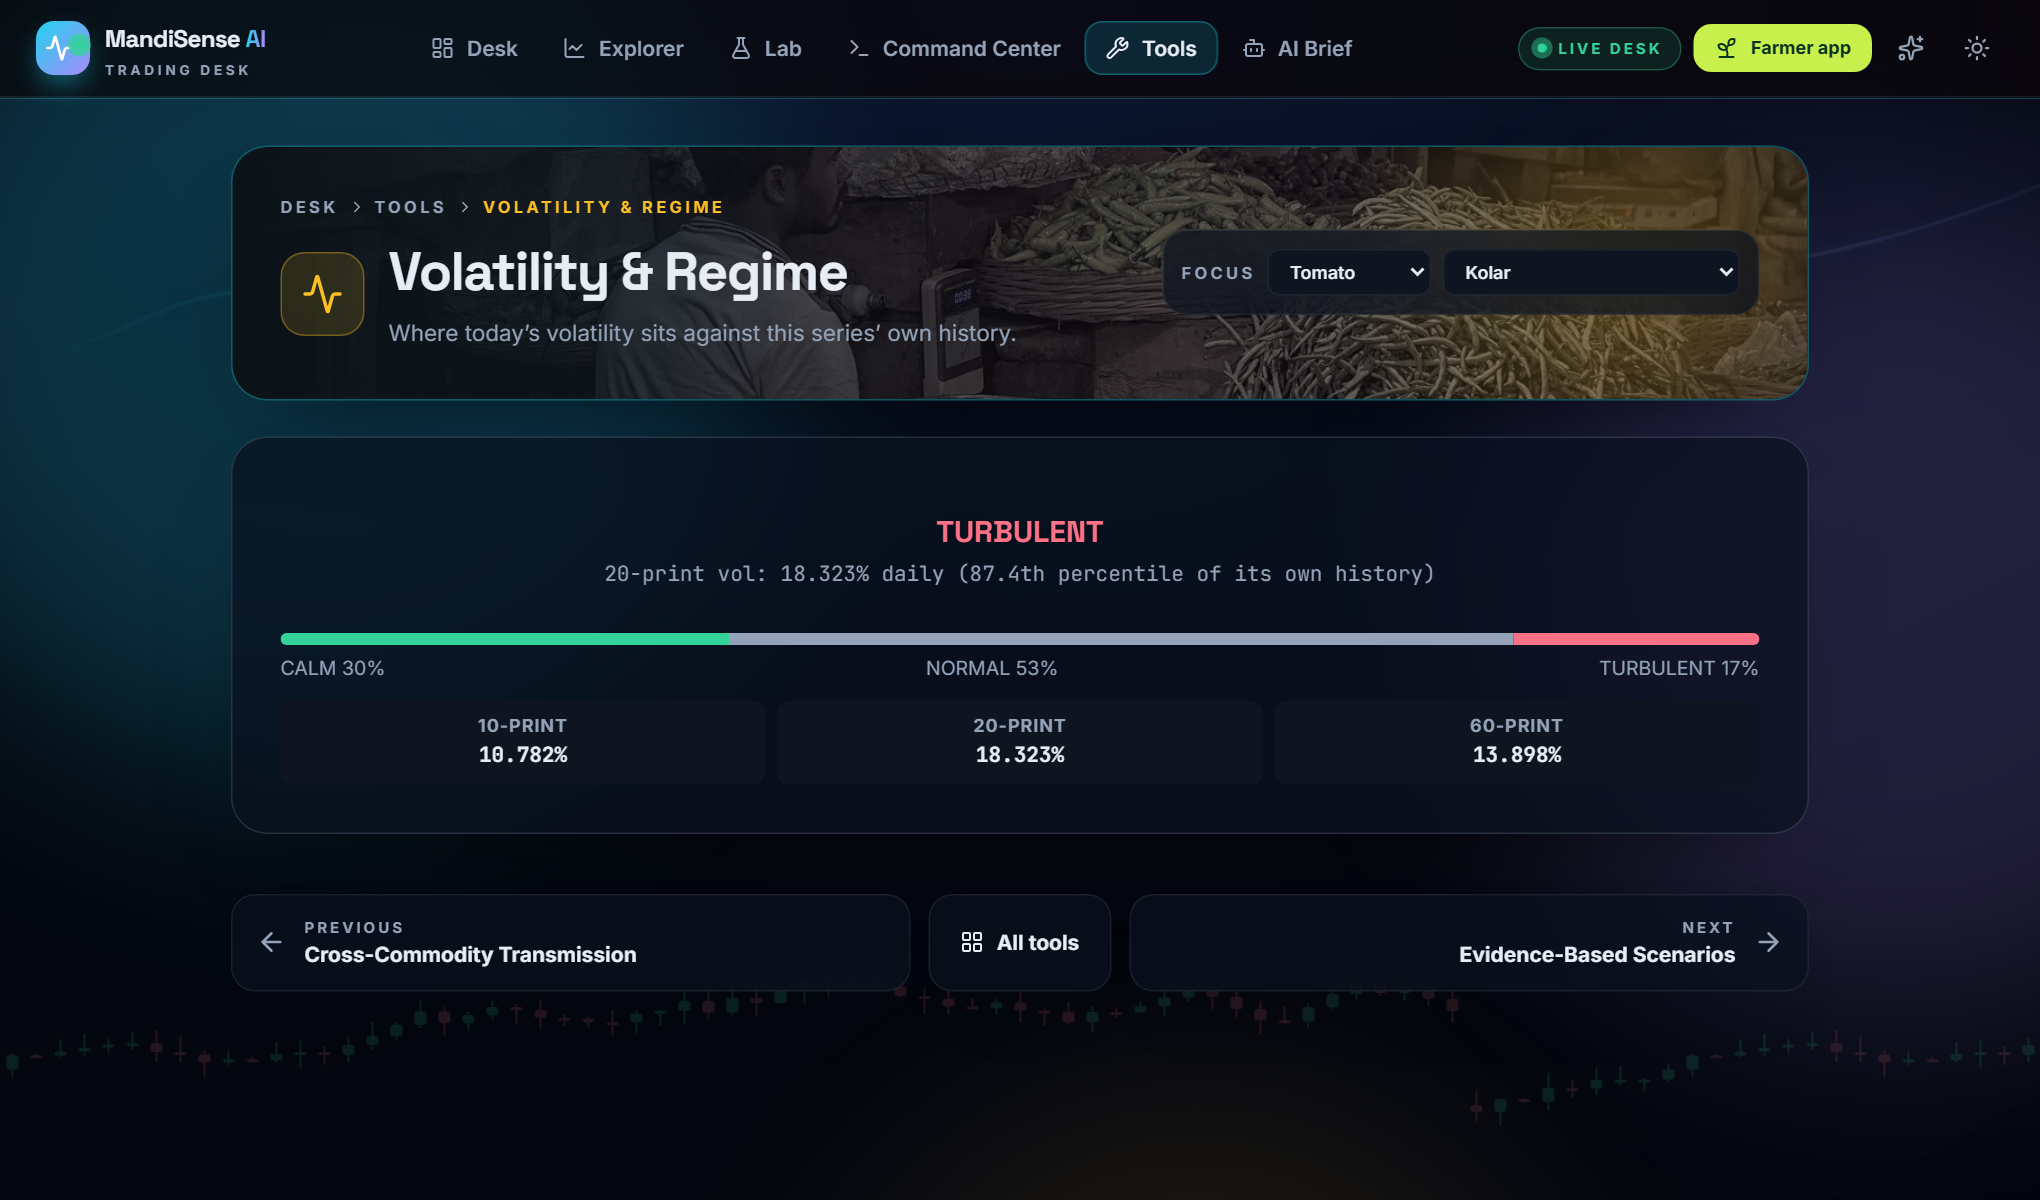
\includegraphics[width=0.93\linewidth]{figures/shot_w_volatility.png}}\\[0.5mm]{\footnotesize (b) Price volatility by commodity and market}
\caption{(a) Cross-commodity transmission. (b) Price volatility by commodity and market.}
\label{fig:sc-w-transmission}
\end{figure}

The transmission page shows the estimated response of one crop to a shock in another. When the evidence is too thin the page says so and shows no number, which is the withholding behaviour described in Section~\ref{sec:transmission}.

Rolling volatility of each series, which the farmer pages translate into a plain warning when a price is unusually unsettled.

\begin{figure}[!t]
\centering
\fbox{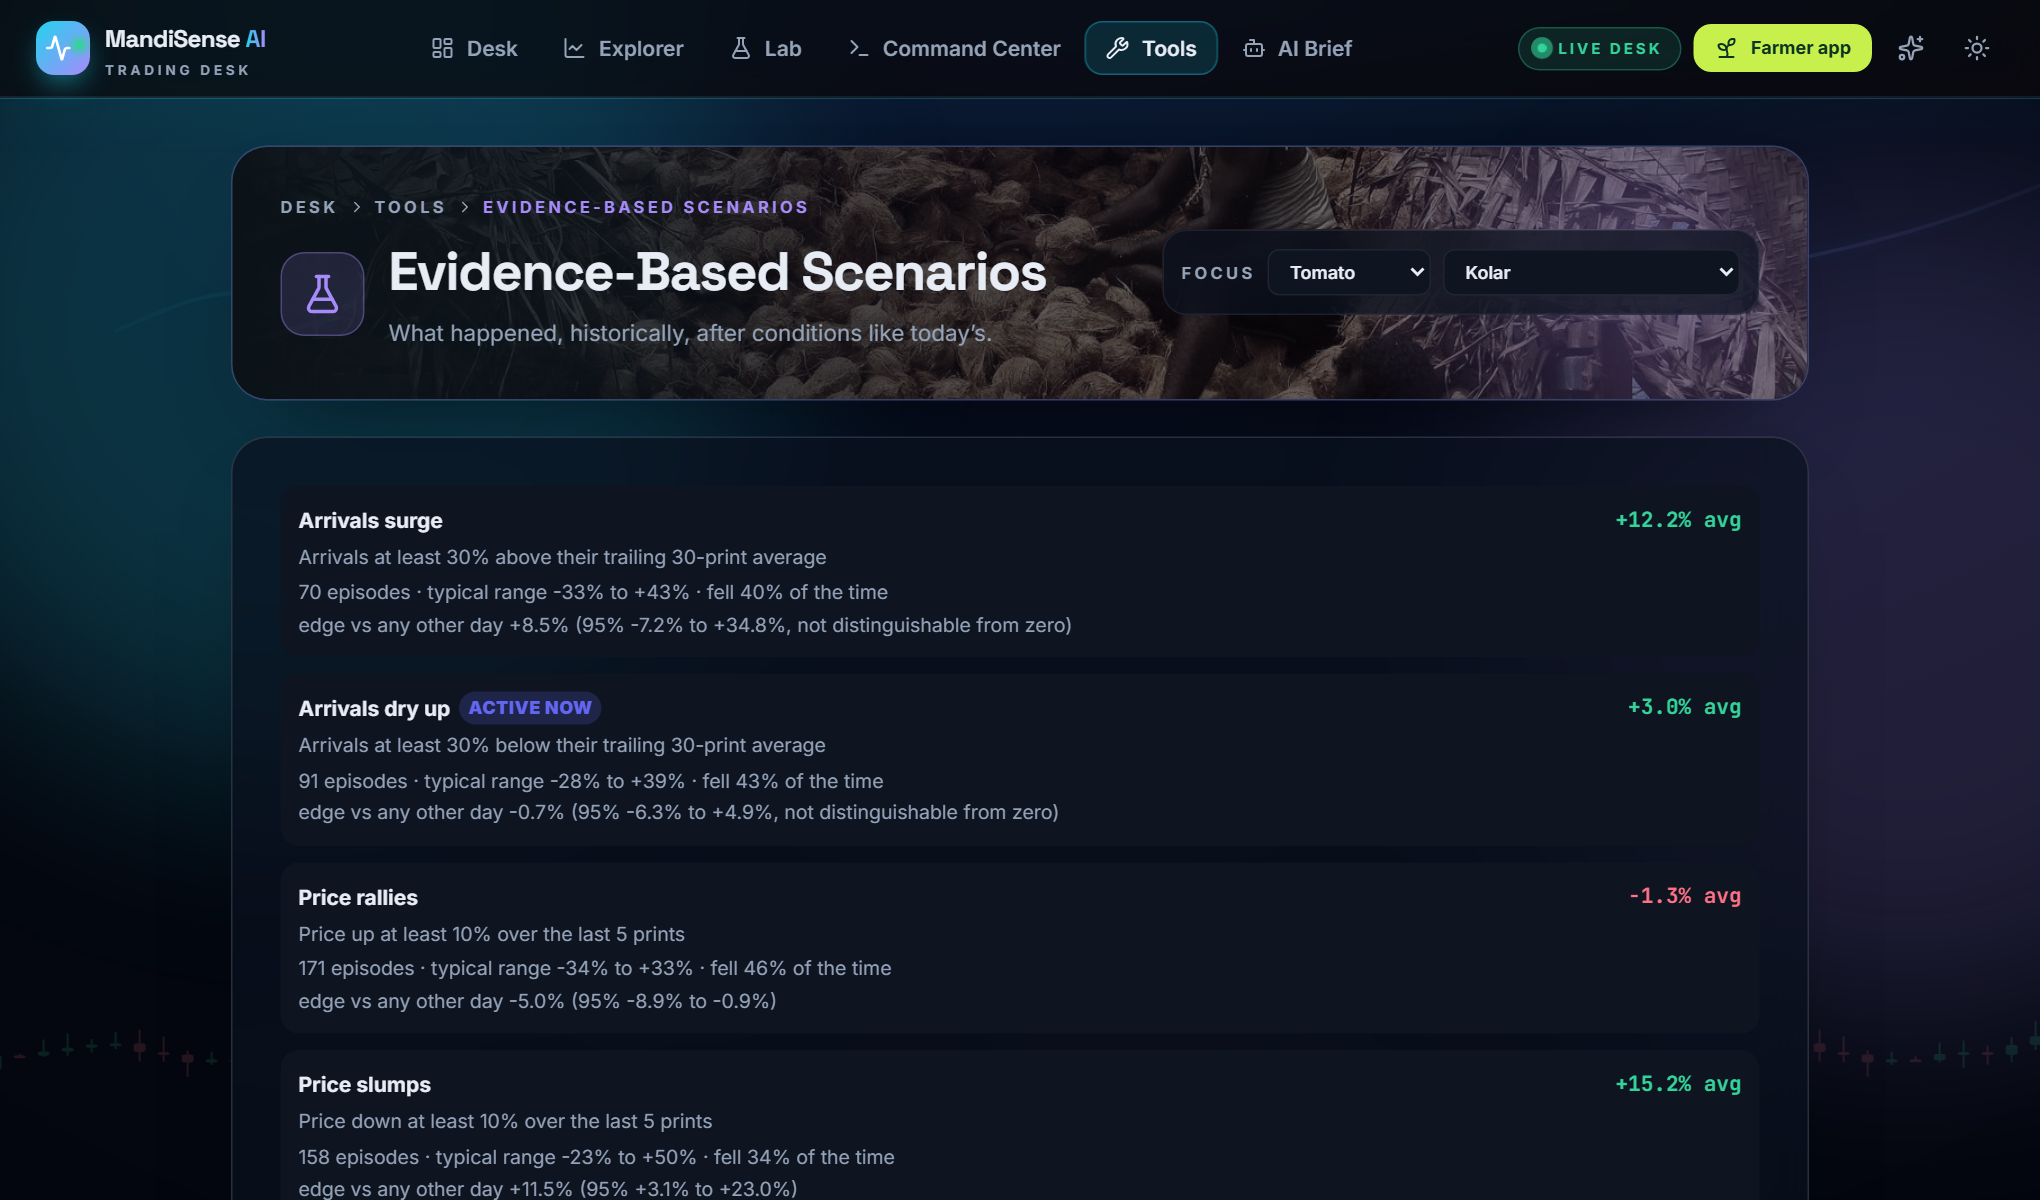
\includegraphics[width=0.93\linewidth]{figures/shot_w_scenarios.png}}\\[0.5mm]{\footnotesize (a) Scenario analysis for the revenue of a sale plan}
\medskip
\fbox{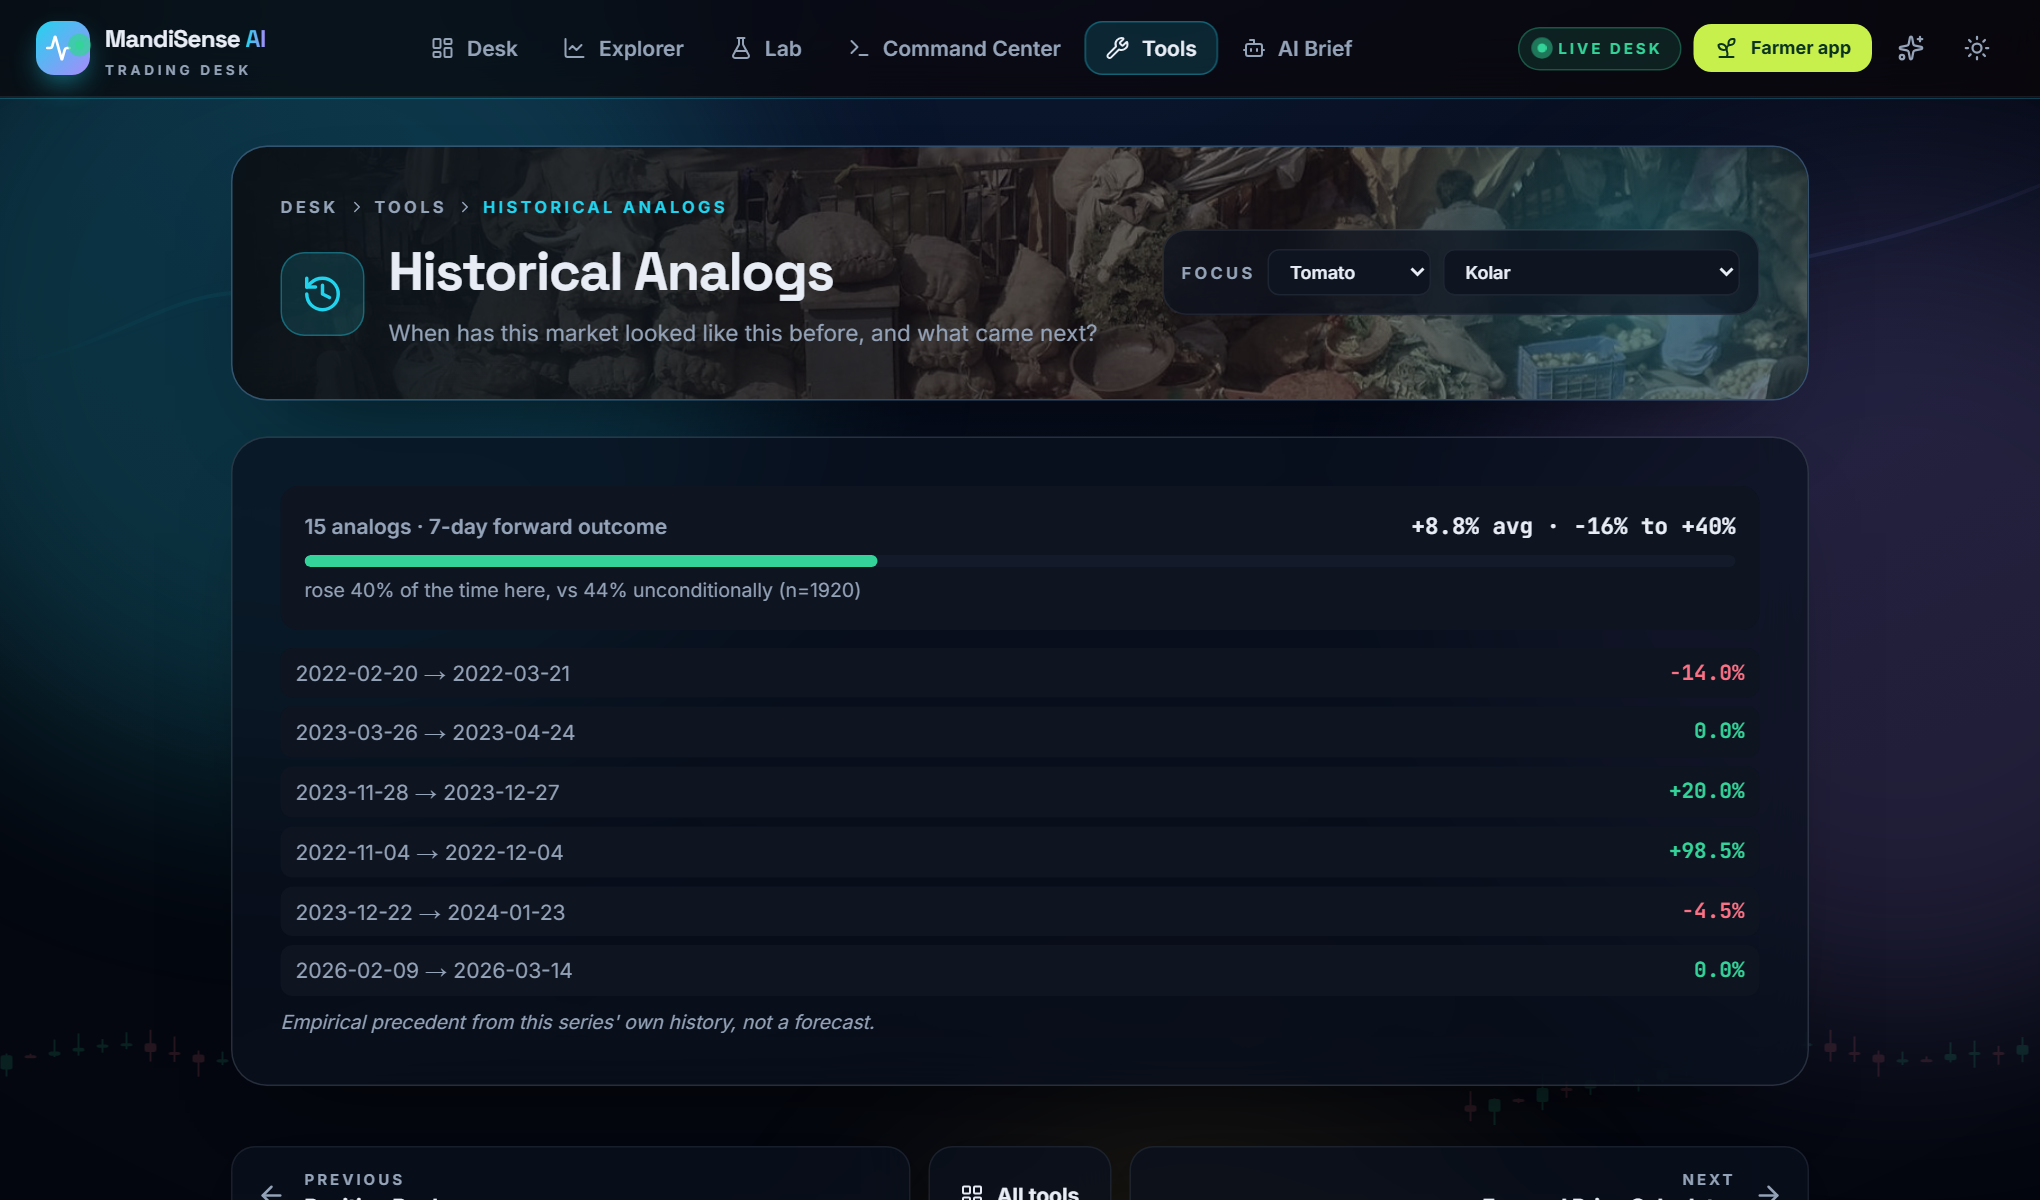
\includegraphics[width=0.93\linewidth]{figures/shot_w_analogs.png}}\\[0.5mm]{\footnotesize (b) Analog days: past days that resembled today}
\caption{(a) Scenario analysis for the revenue of a sale plan. (b) Analog days: past days that resembled today.}
\label{fig:sc-w-scenarios}
\end{figure}

The tool changes transport cost, shrinkage and price in turn and shows how the recommended choice and its revenue respond.

The page finds earlier days with a similar price pattern and shows what followed, as an aid to judgement and not as a forecast.

\begin{figure}[!t]
\centering
\fbox{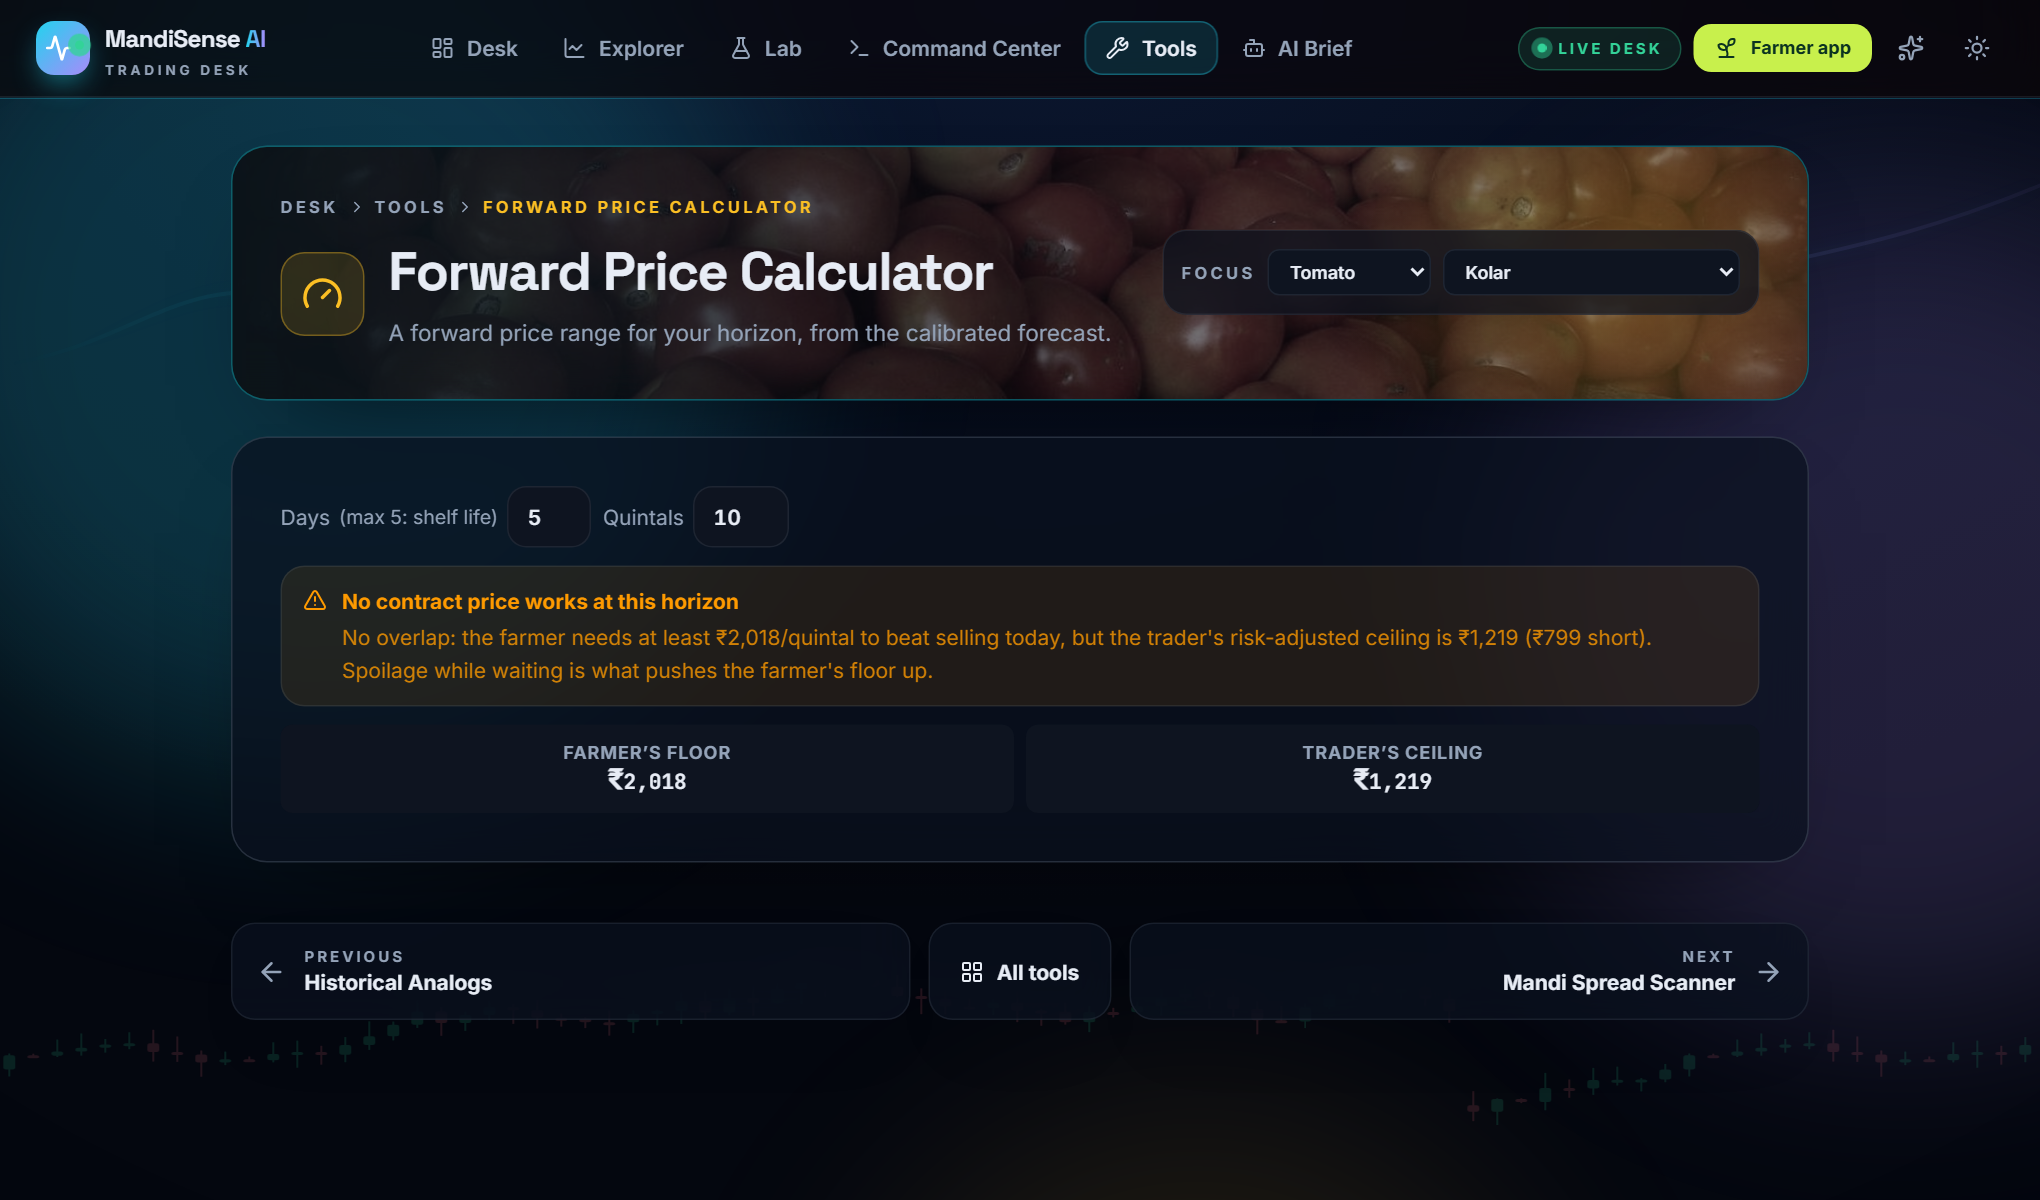
\includegraphics[width=0.93\linewidth]{figures/shot_w_forward.png}}\\[0.5mm]{\footnotesize (a) Forward price view}
\medskip
\fbox{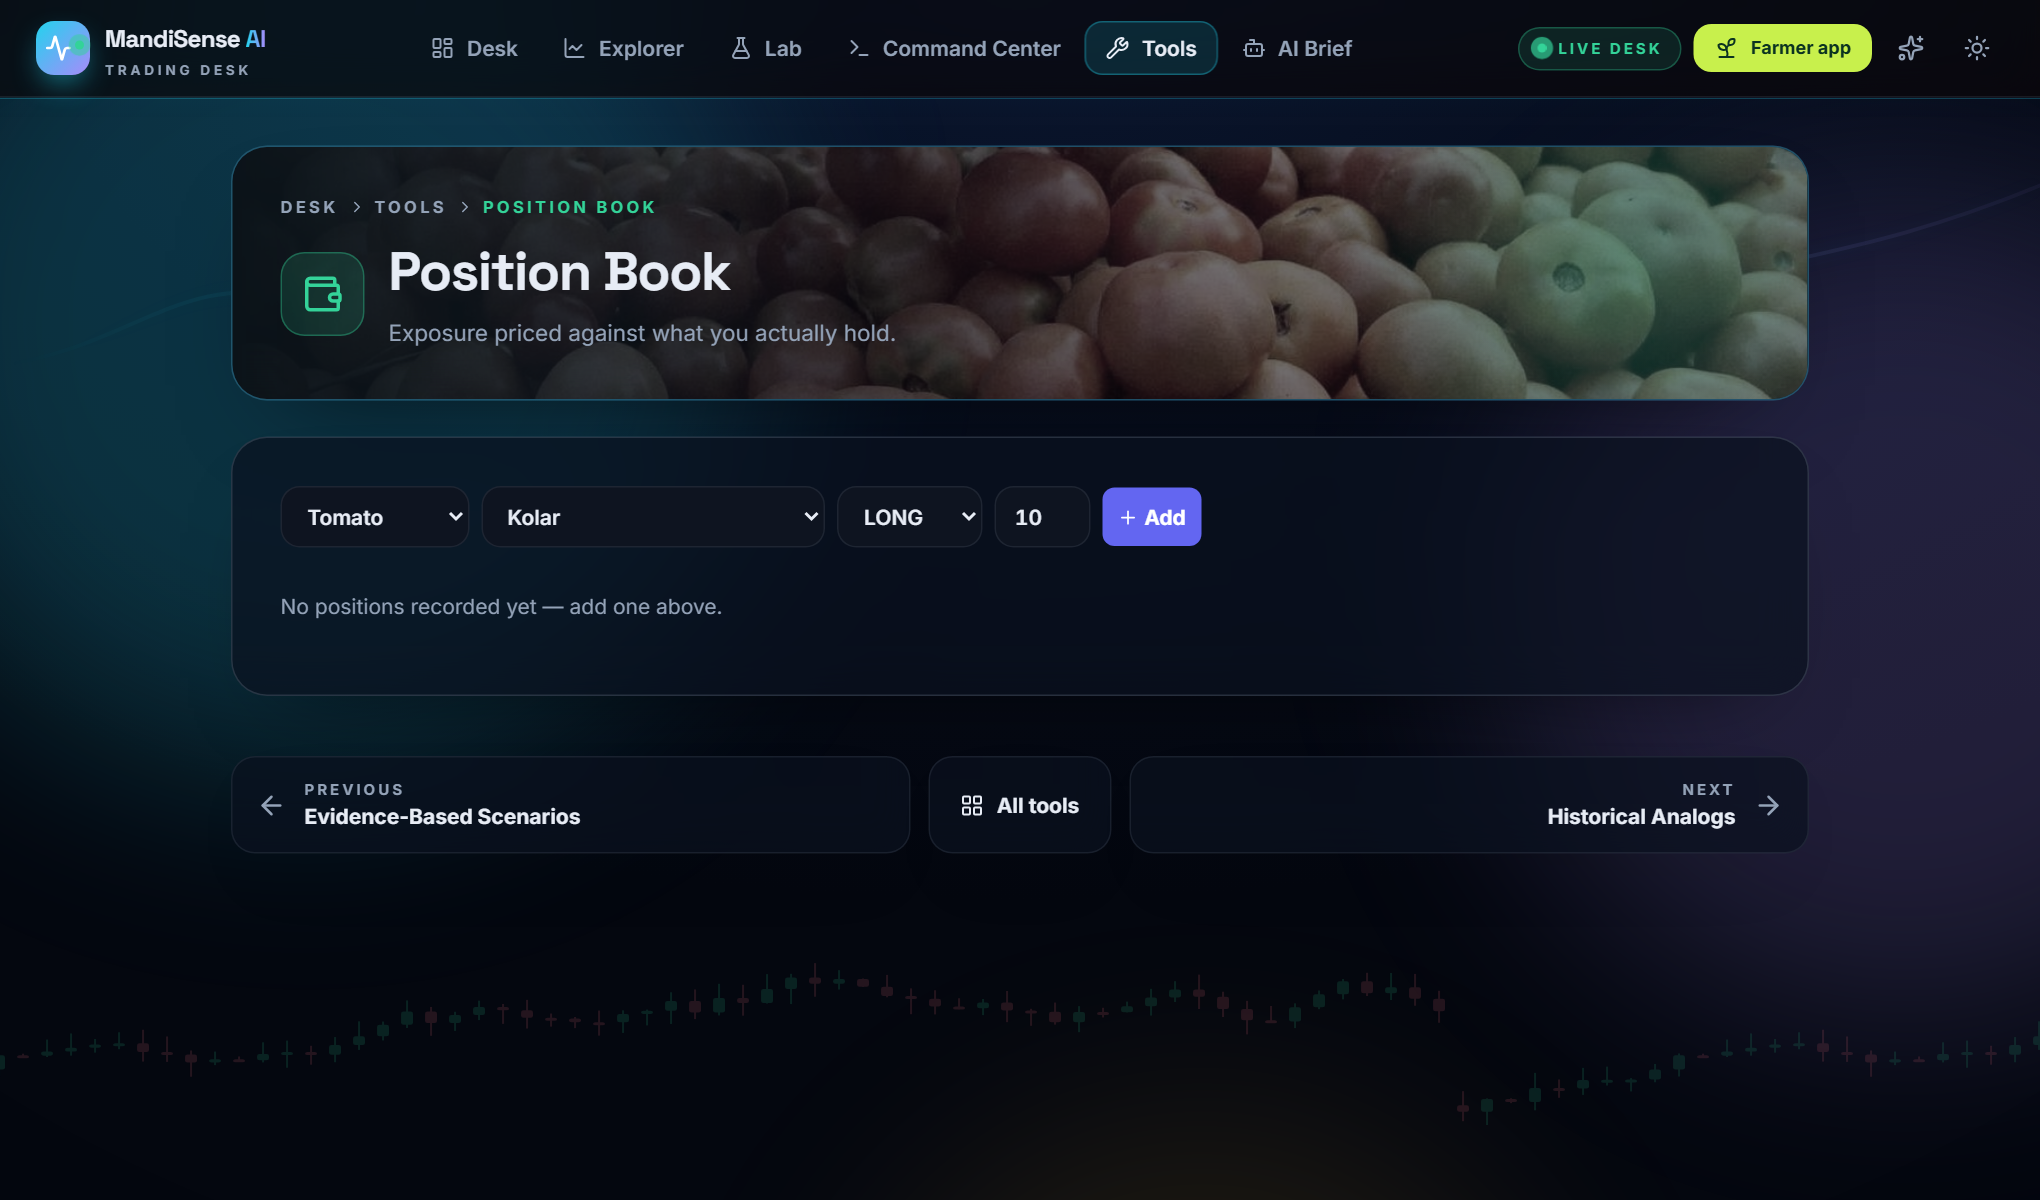
\includegraphics[width=0.93\linewidth]{figures/shot_w_positions.png}}\\[0.5mm]{\footnotesize (b) Positions: the sales a trader is tracking}
\caption{(a) Forward price view. (b) Positions: the sales a trader is tracking.}
\label{fig:sc-w-forward}
\end{figure}

A forecast with its interval for the coming days, with the forecasting model named on the page.

A small ledger of intended sales with their marked-to-market value.

\begin{figure}[!t]
\centering
\fbox{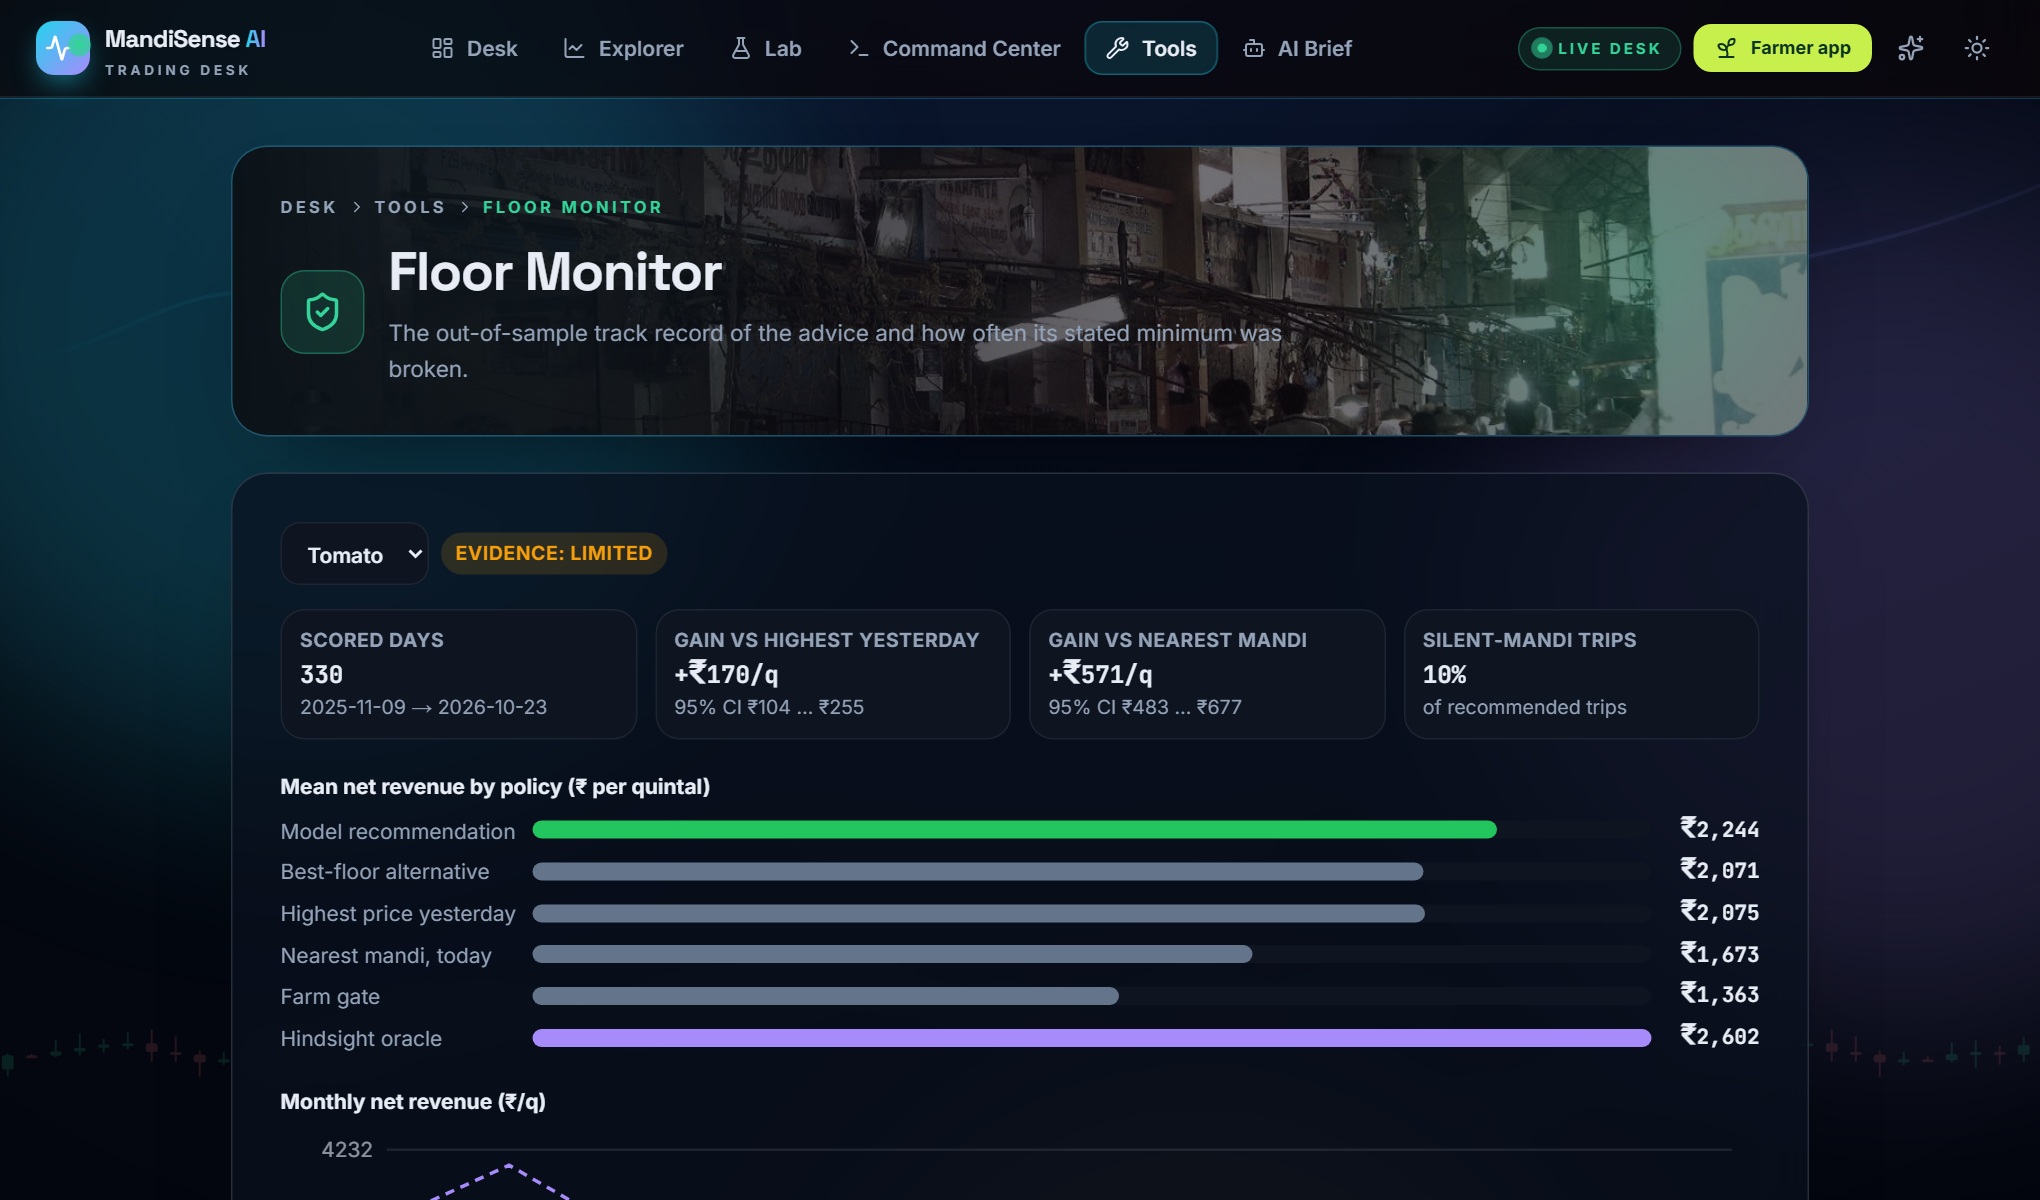
\includegraphics[width=0.93\linewidth]{figures/shot_w_floormon.png}}\\[0.5mm]{\footnotesize (a) Floor monitor: how often the revenue floor has held}
\medskip
\fbox{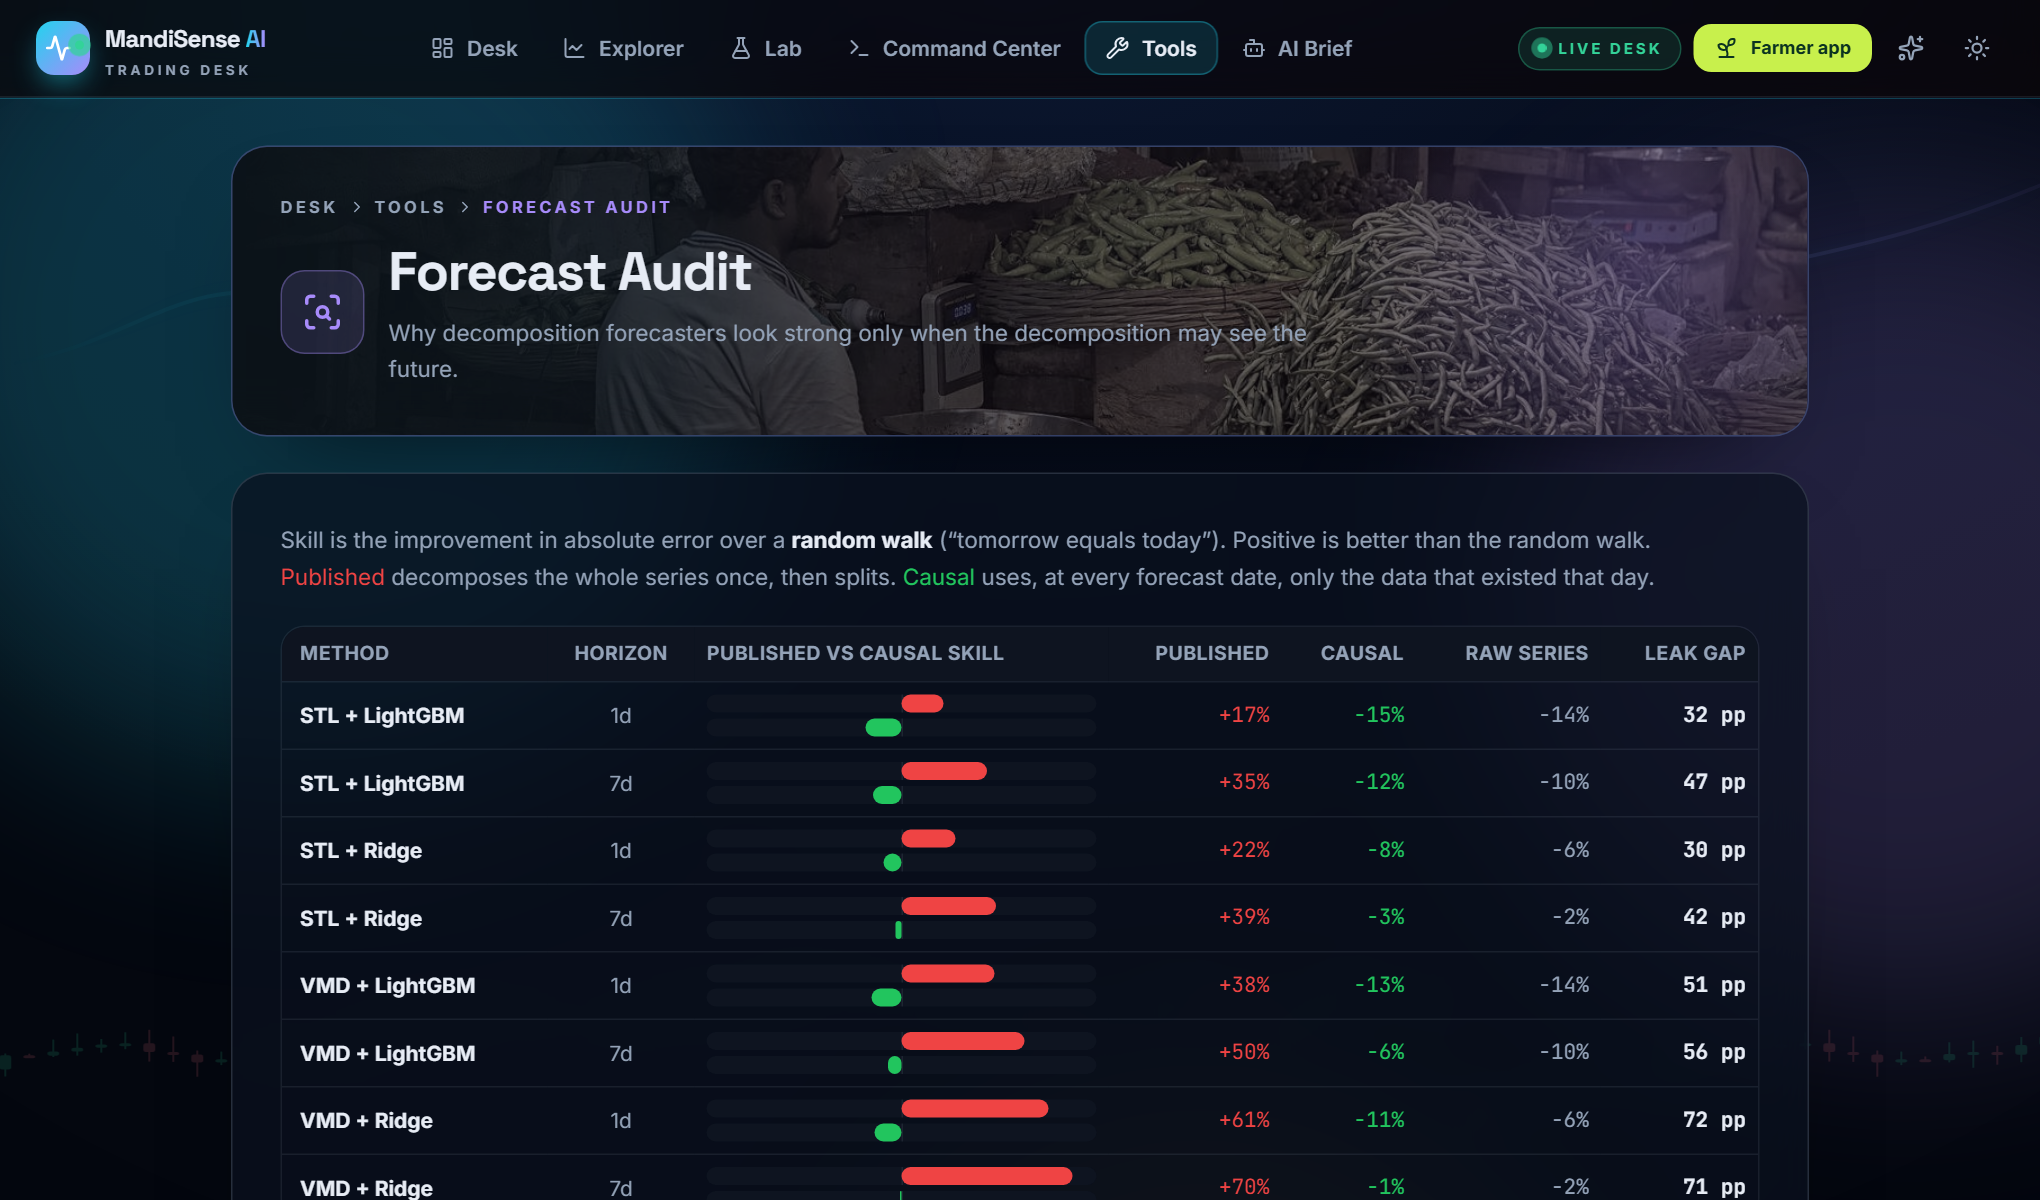
\includegraphics[width=0.93\linewidth]{figures/shot_w_audit.png}}\\[0.5mm]{\footnotesize (b) Forecast audit}
\caption{(a) Floor monitor: how often the revenue floor has held. (b) Forecast audit.}
\label{fig:sc-w-floormon}
\end{figure}

The monitor tracks, day by day, whether realised revenue stayed above the stated floor and shows the running violation rate against its target, so a drift in calibration is visible.

The audit compares each forecaster with the naive predictor on the days it was used and shows where it adds nothing.

\begin{figure}[!t]
\centering
\fbox{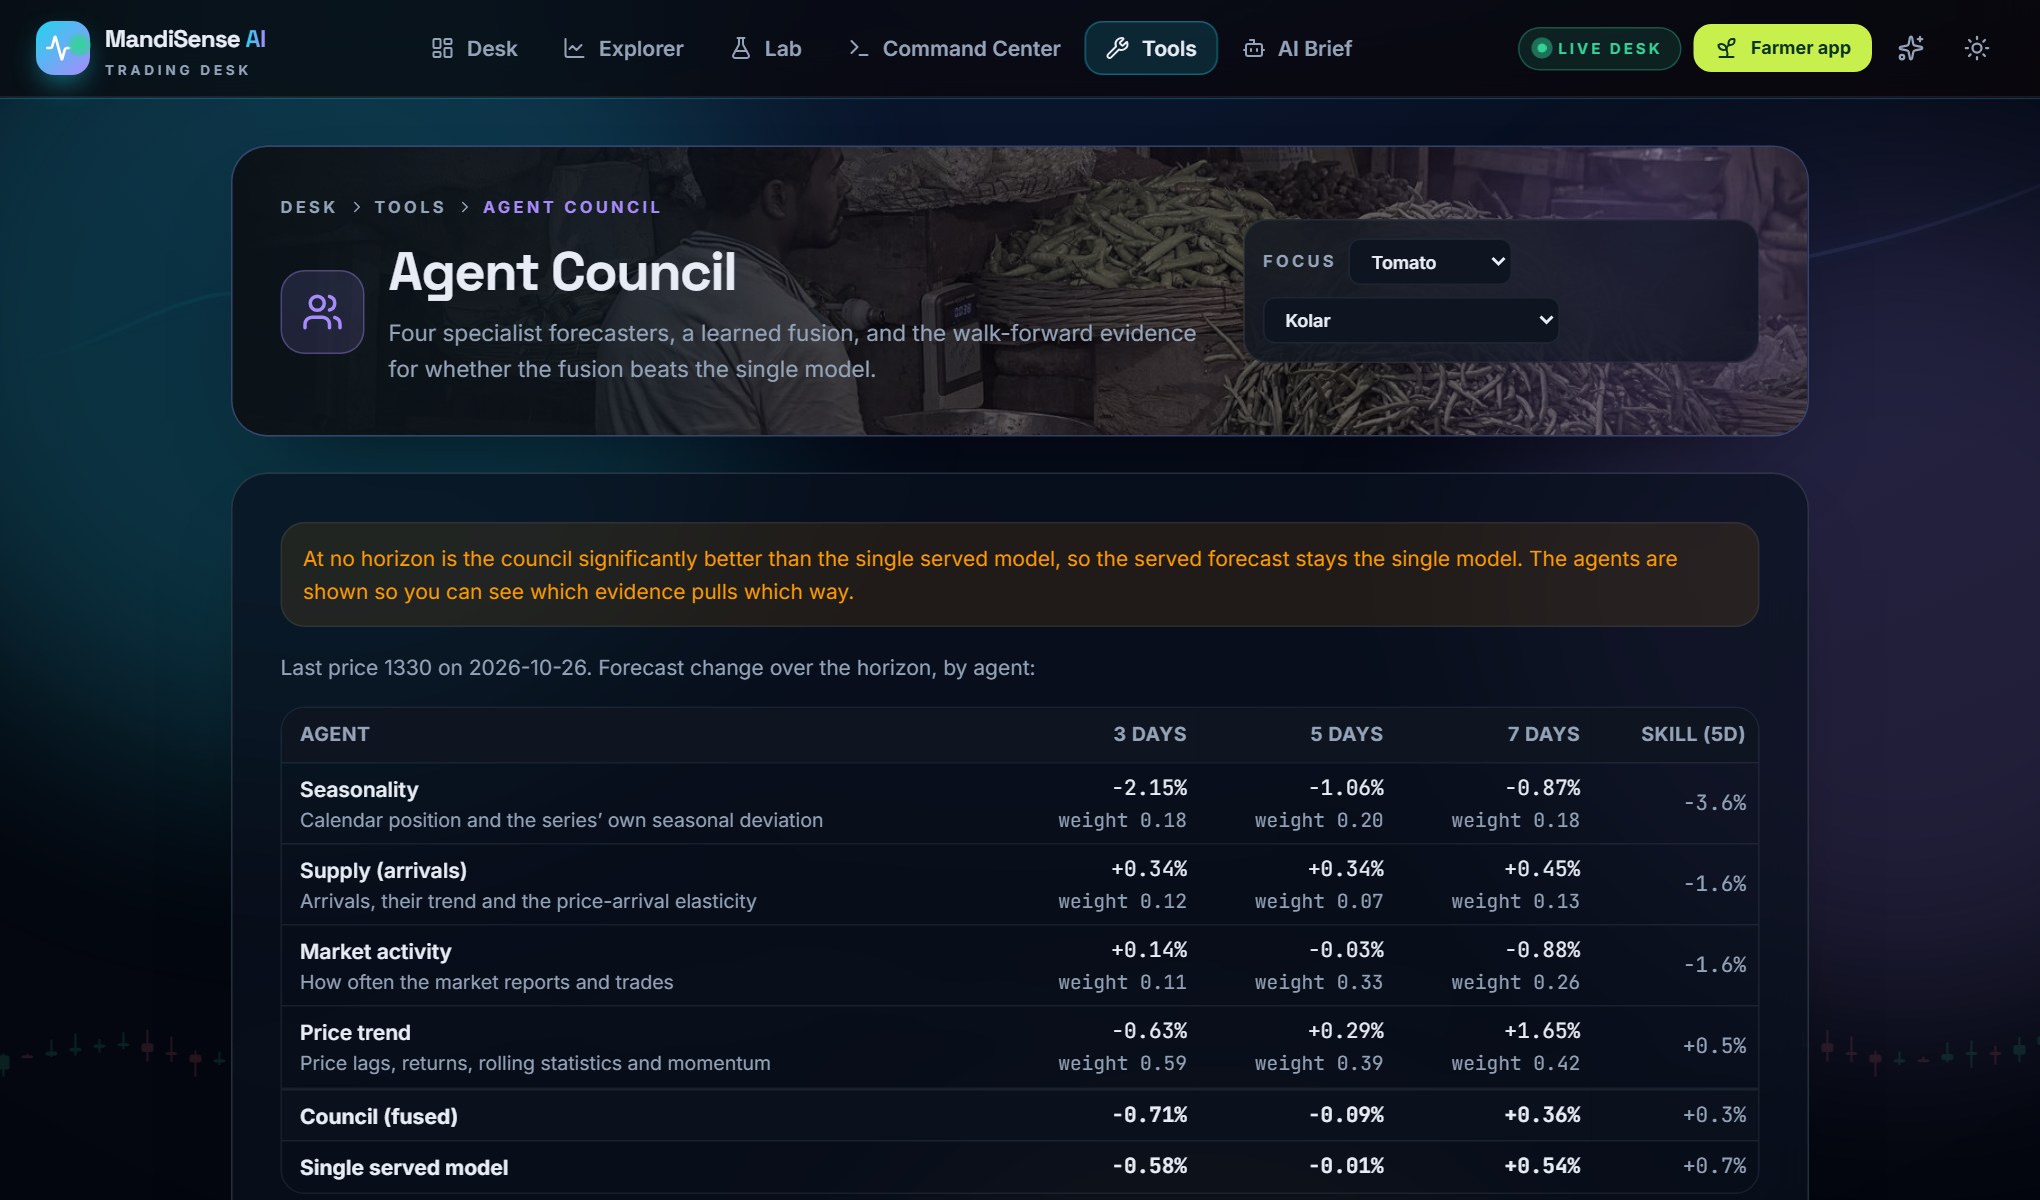
\includegraphics[width=0.93\linewidth]{figures/shot_w_council.png}}\\[0.5mm]{\footnotesize (a) Agent council: specialist forecasters and their weights}
\medskip
\fbox{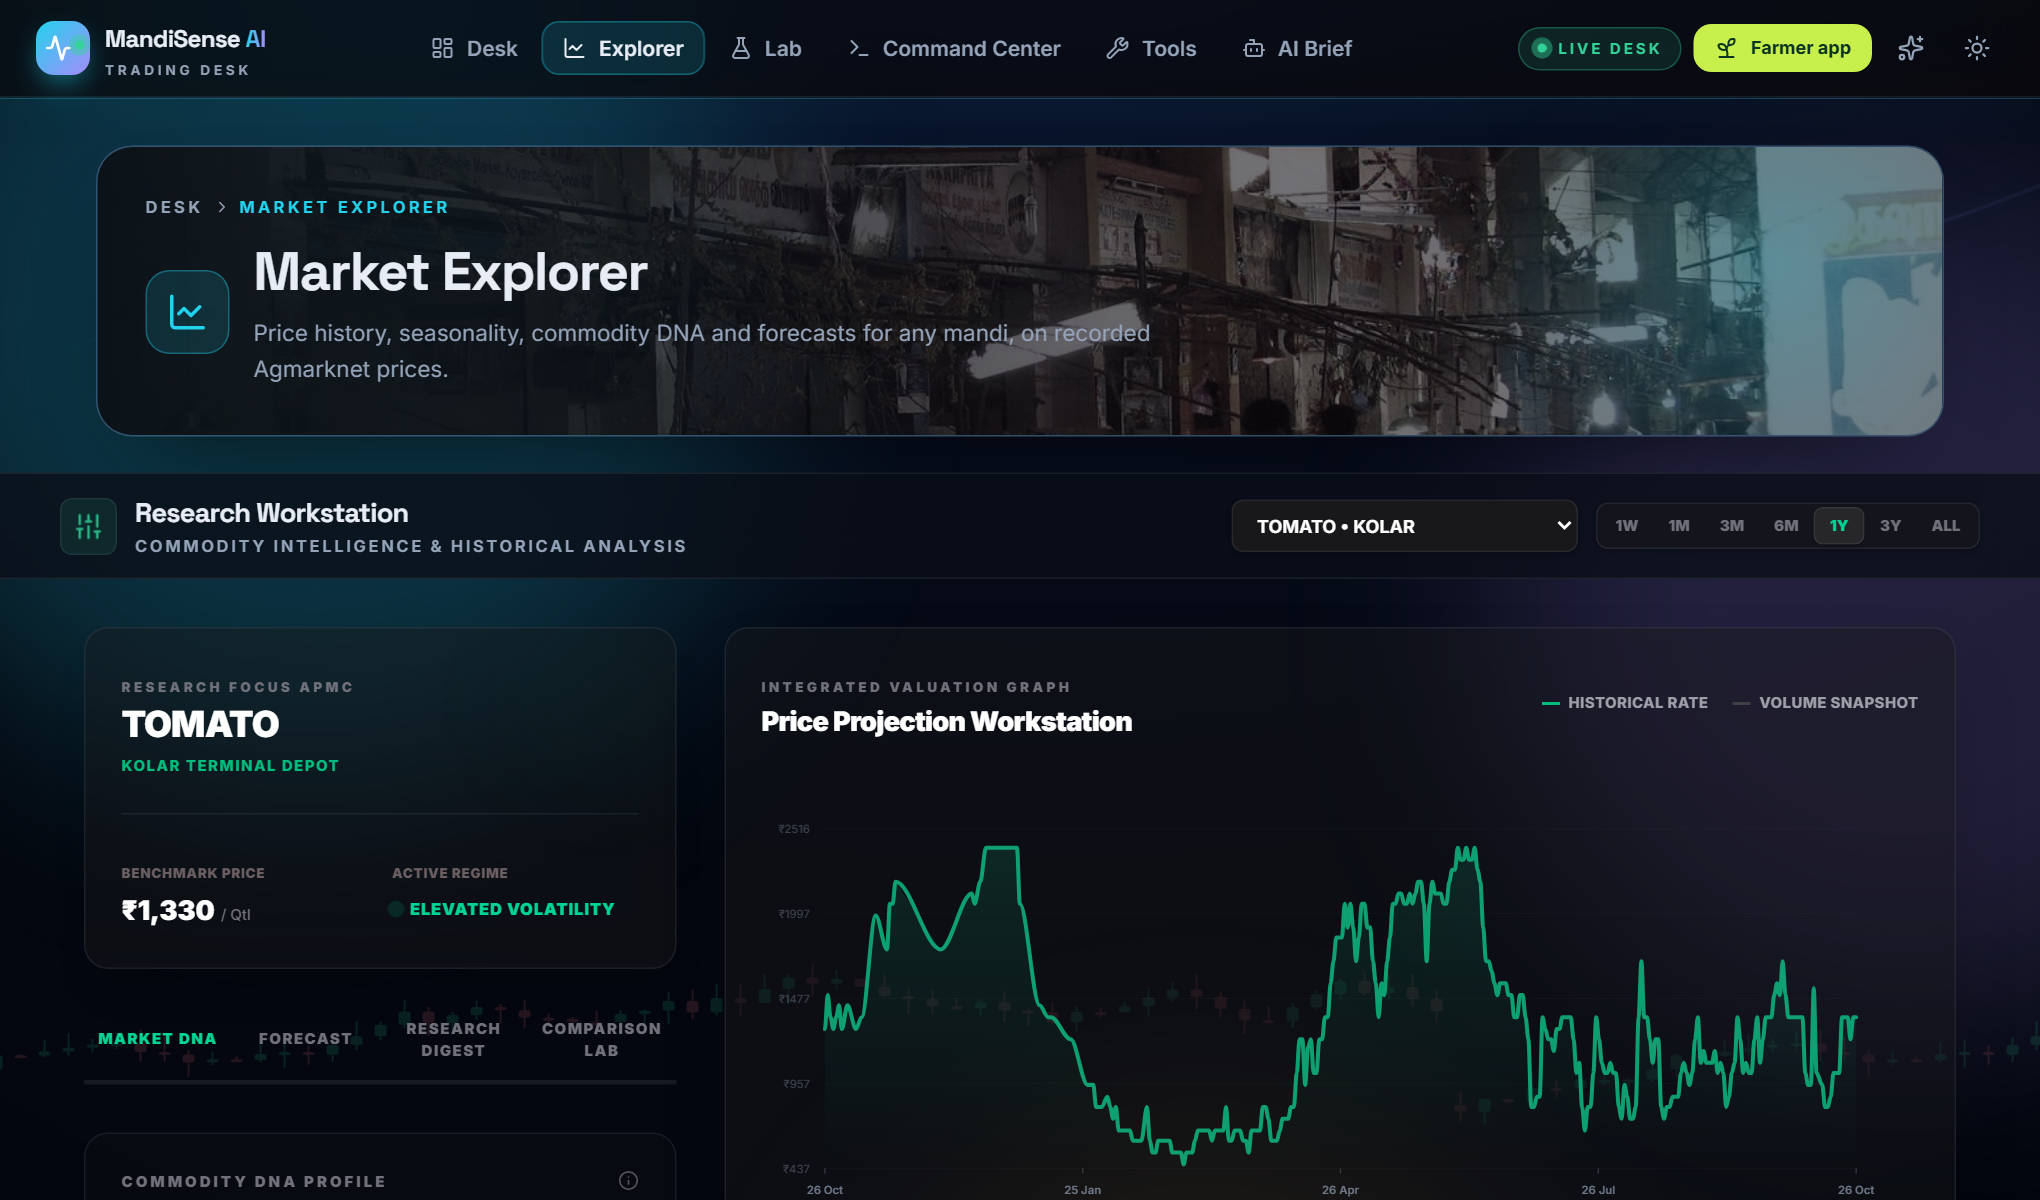
\includegraphics[width=0.93\linewidth]{figures/shot_w_explorer.png}}\\[0.5mm]{\footnotesize (b) Market explorer: any crop, any market, any period}
\caption{(a) Agent council: specialist forecasters and their weights. (b) Market explorer: any crop, any market, any period.}
\label{fig:sc-w-council}
\end{figure}

The council page shows the specialist forecasters and the weight each currently carries, the object of Section~\ref{sec:architecture}.

The explorer lets a user chart raw reported prices and arrivals, with gaps in reporting shown as gaps.

\begin{figure}[!t]
\centering
\fbox{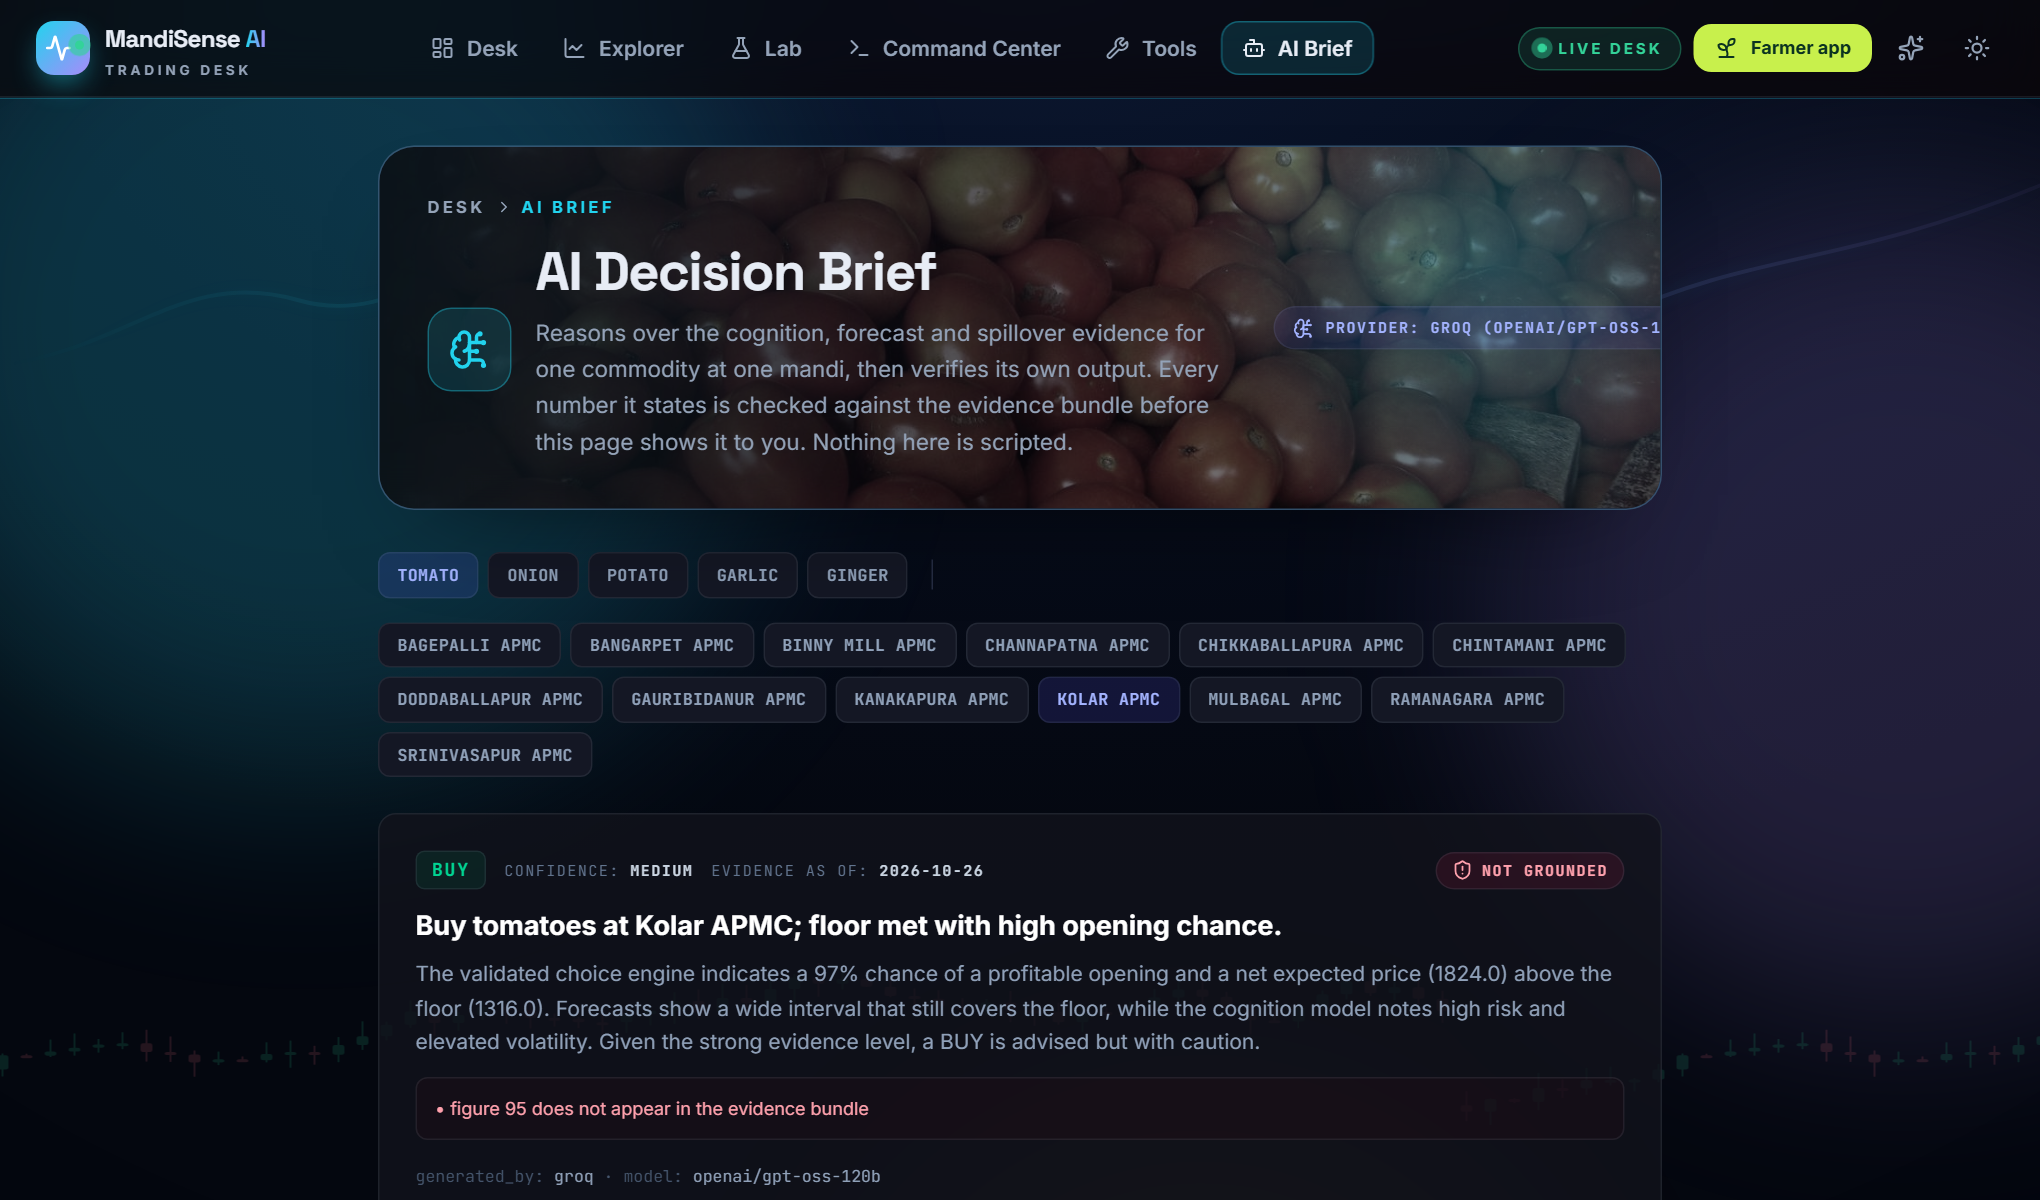
\includegraphics[width=0.93\linewidth]{figures/shot_w_aibrief.png}}\\[0.5mm]{\footnotesize (a) The AI brief: a written summary checked against the evidence}
\medskip
\fbox{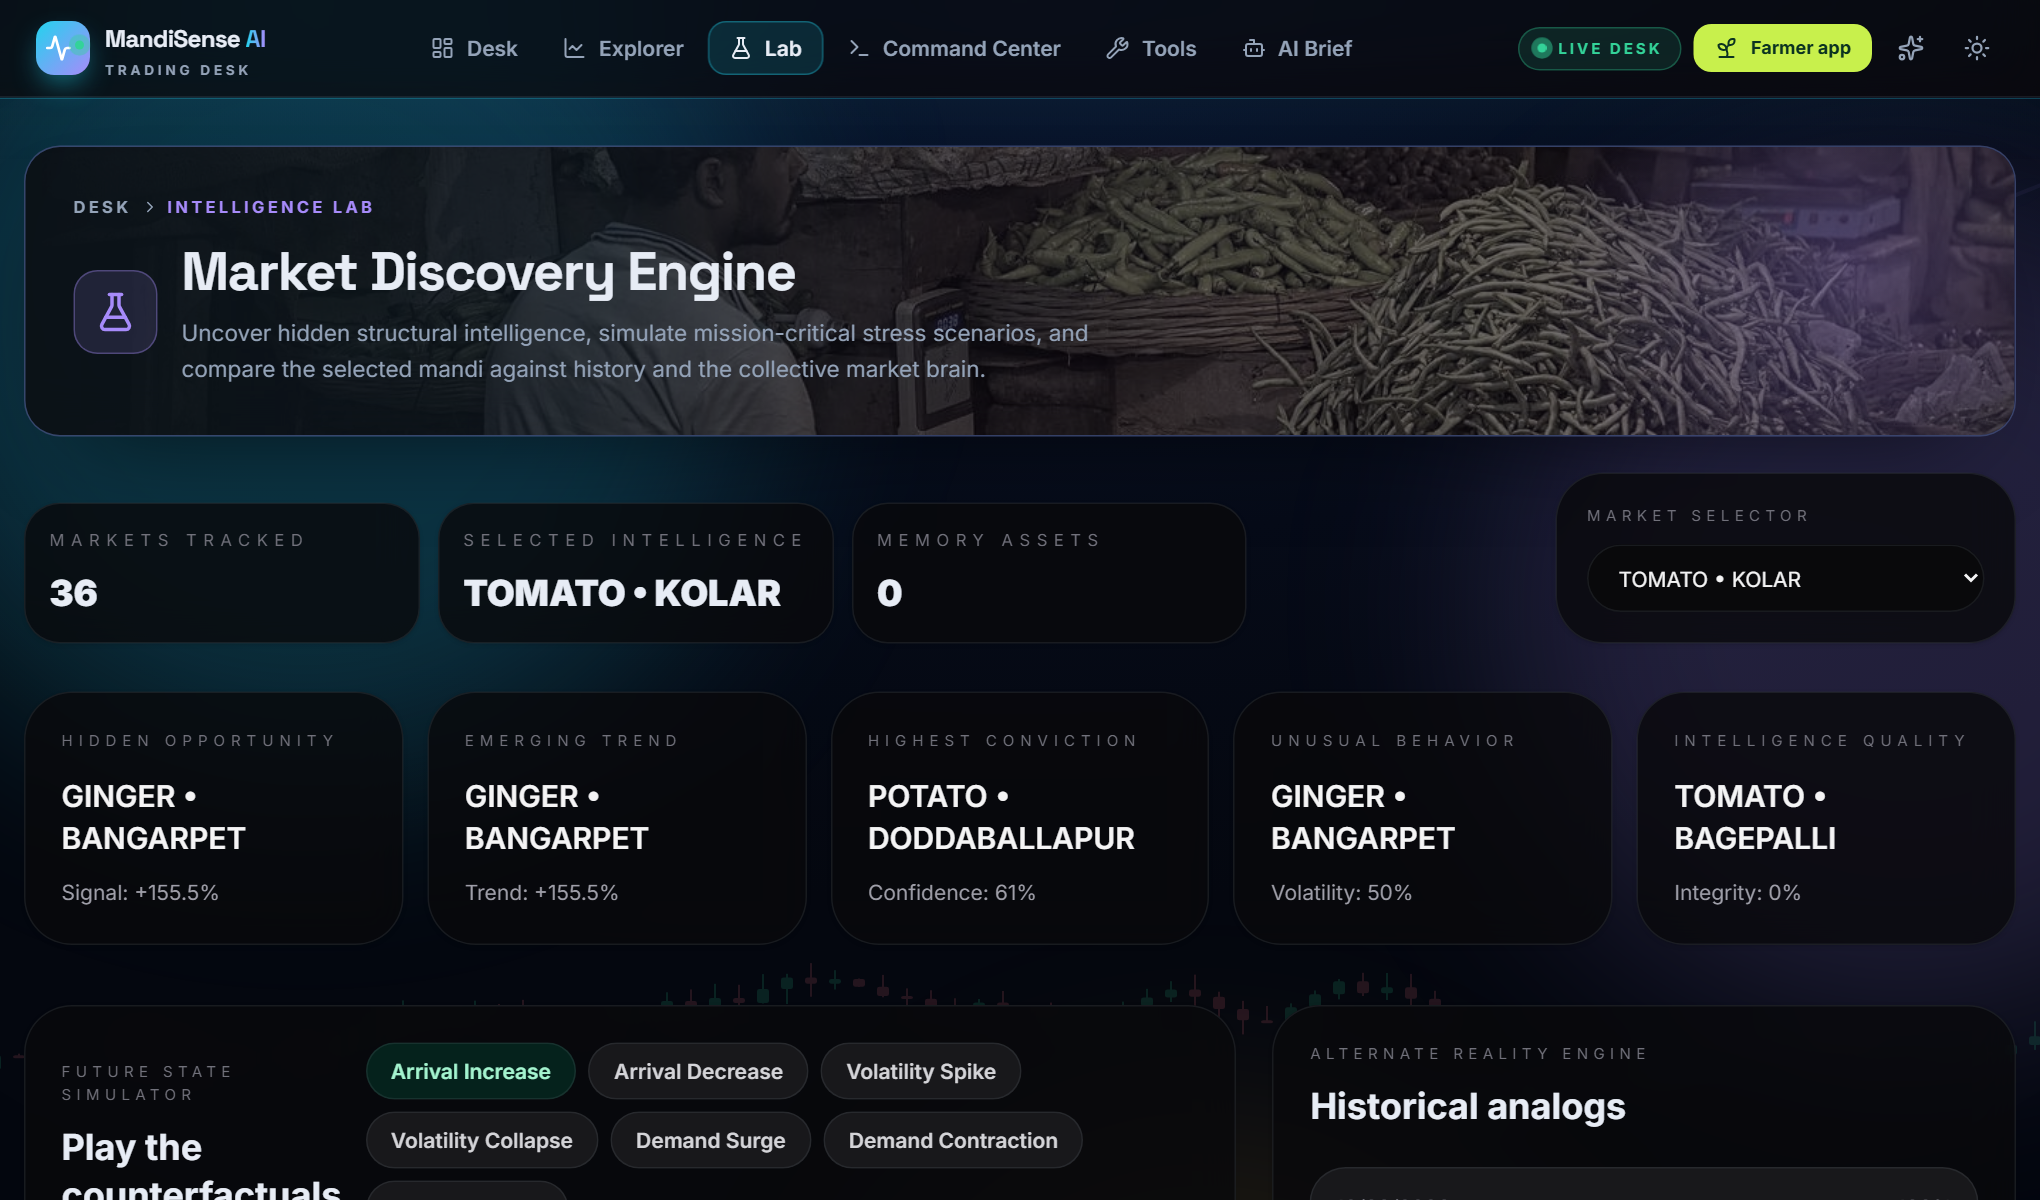
\includegraphics[width=0.93\linewidth]{figures/shot_w_lab.png}}\\[0.5mm]{\footnotesize (b) Intelligence lab: experiment summaries}
\caption{(a) The AI brief: a written summary checked against the evidence. (b) Intelligence lab: experiment summaries.}
\label{fig:sc-w-aibrief}
\end{figure}

The brief is written by the language model of Section~\ref{sec:llm} and every figure in it is checked against the evidence before it is shown. A brief that fails the check is discarded and the page falls back to a plain summary.

The lab page presents the experiment results of Chapter~\ref{ch:results} interactively.

\begin{figure}[!t]
\centering
\fbox{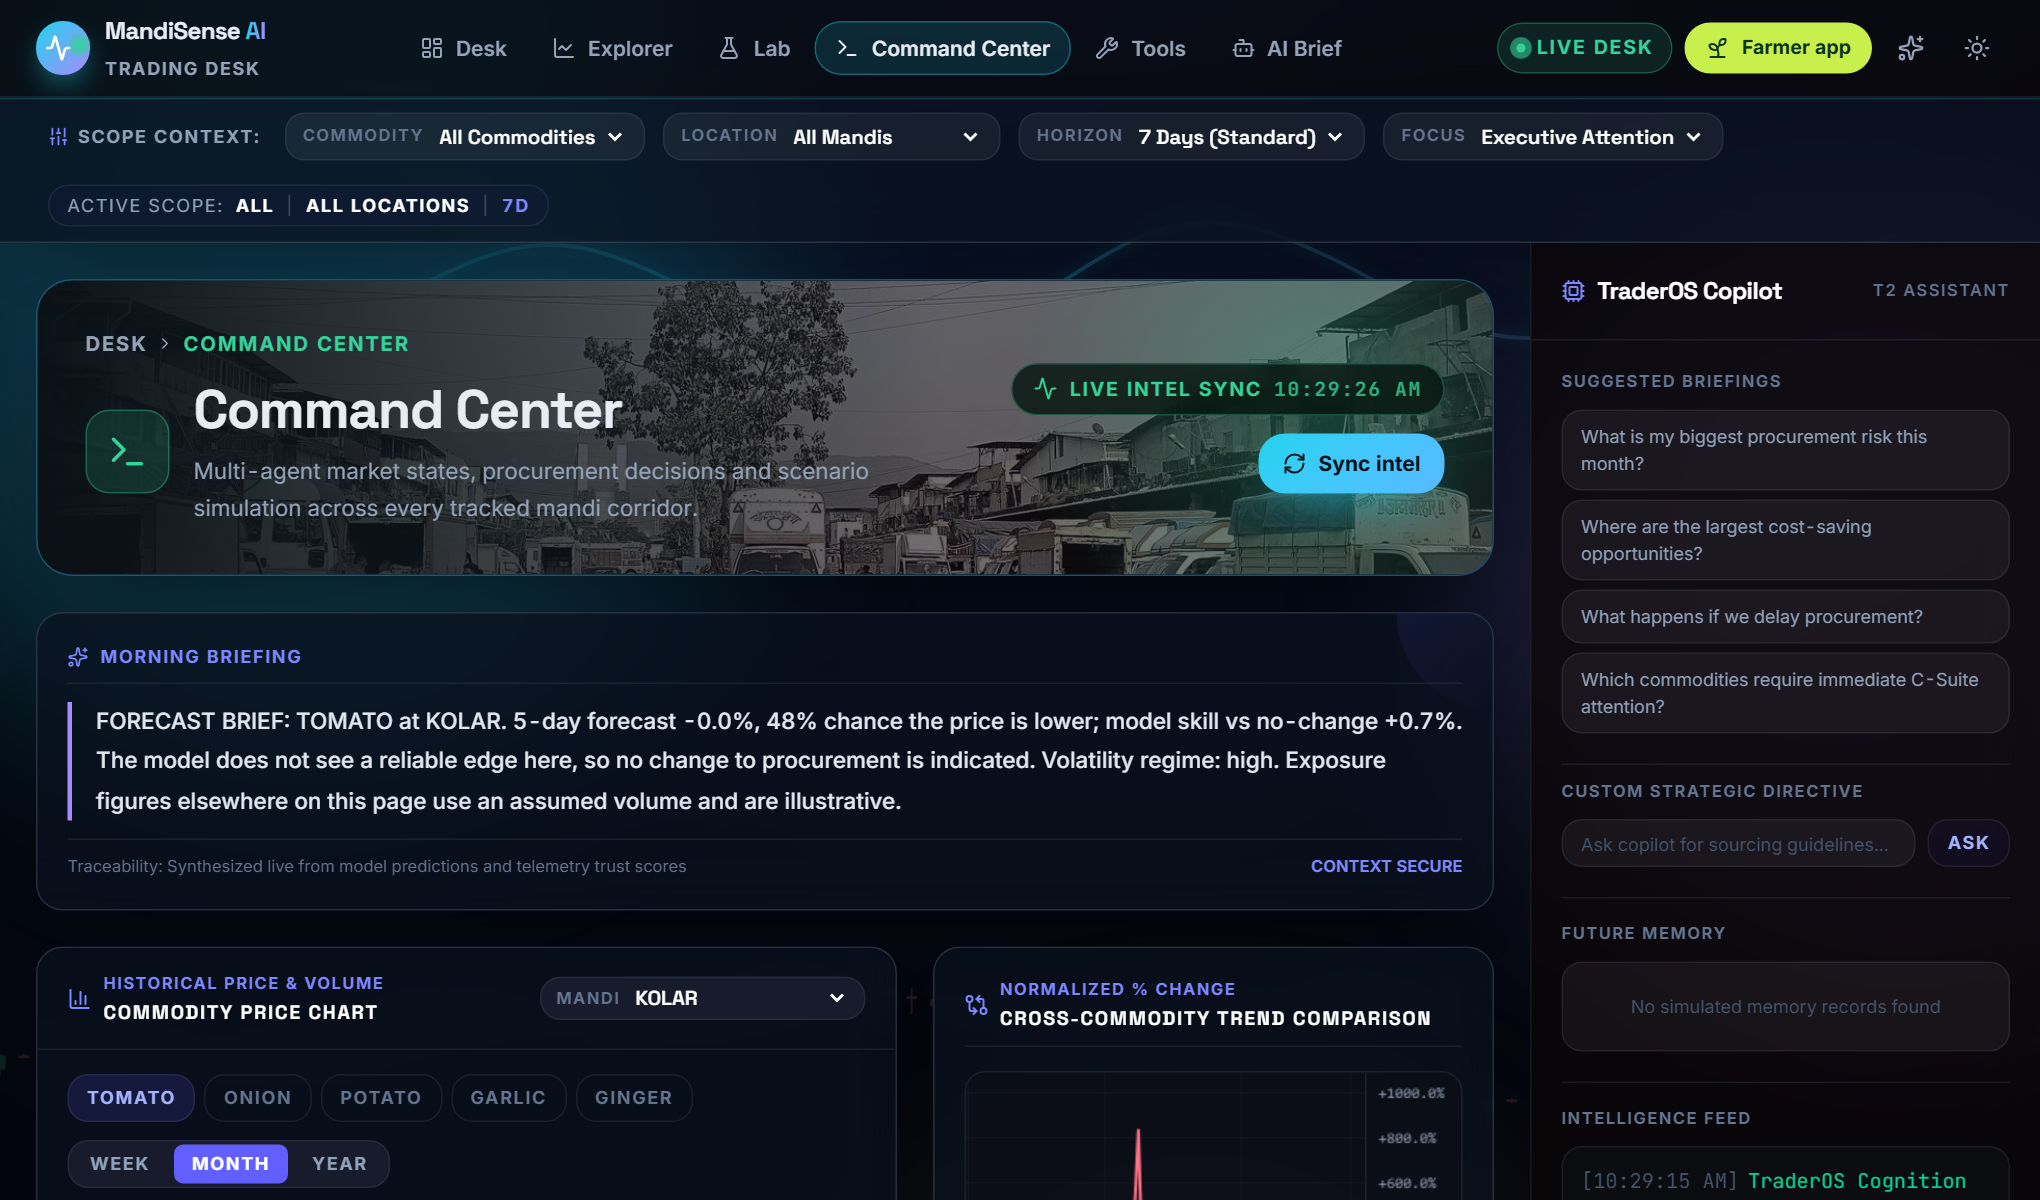
\includegraphics[width=0.93\linewidth]{figures/shot_w_terminal.png}}\\[0.5mm]{\footnotesize (a) Terminal view: dense prices for desk use}
\medskip
\fbox{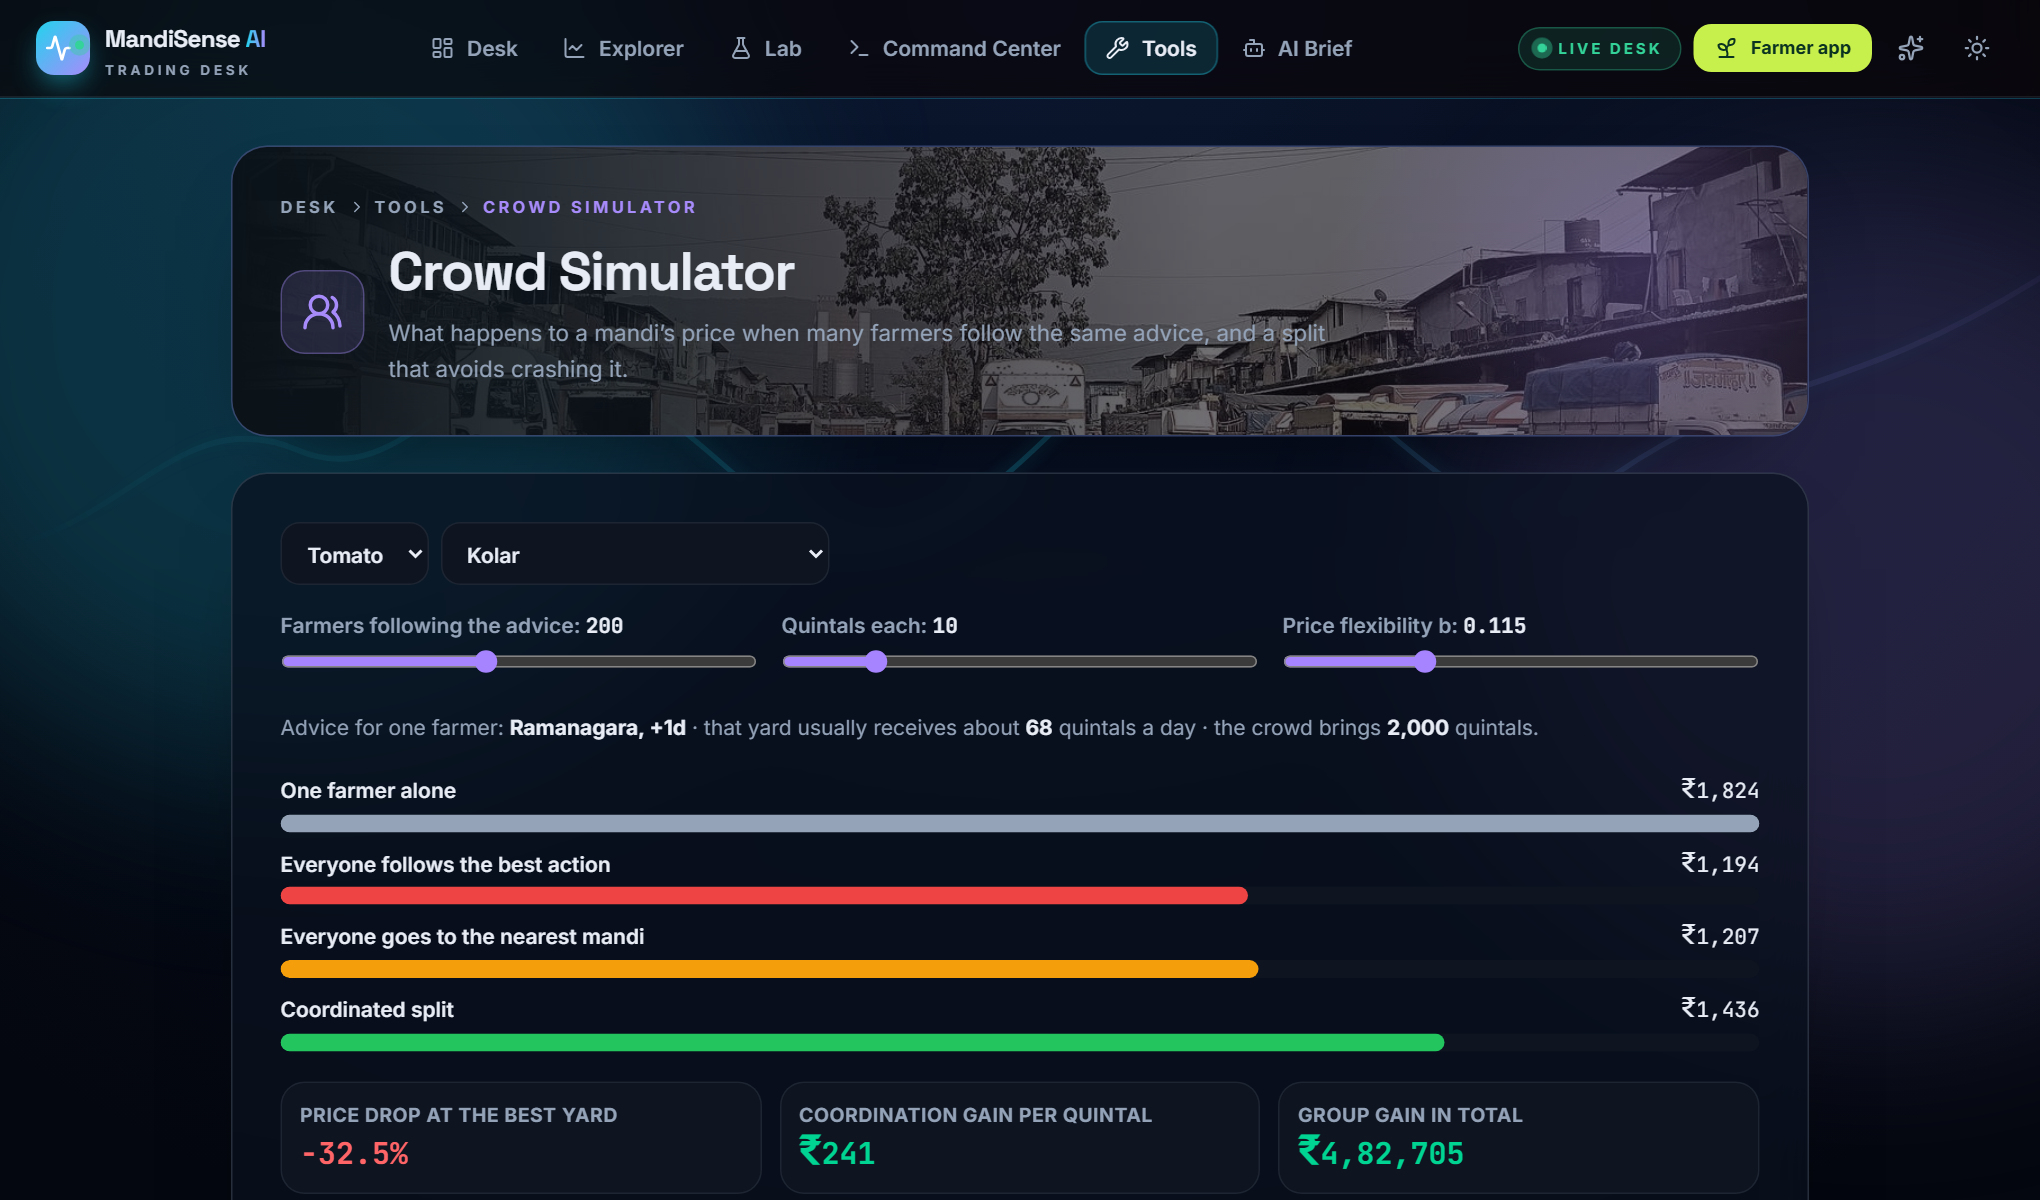
\includegraphics[width=0.93\linewidth]{figures/shot_w_crowd.png}}\\[0.5mm]{\footnotesize (b) Crowd simulator: what happens when many farmers follow the same advice}
\caption{(a) Terminal view: dense prices for desk use. (b) Crowd simulator: what happens when many farmers follow the same advice.}
\label{fig:sc-w-terminal}
\end{figure}

A compact table of the latest price per market, intended to stay open beside other work.

The simulator raises the share of farmers following the advice and shows the net revenue under four policies, using a stated price flexibility (Section~\ref{sec:insight-method}).

\begin{figure}[!t]
\centering
\fbox{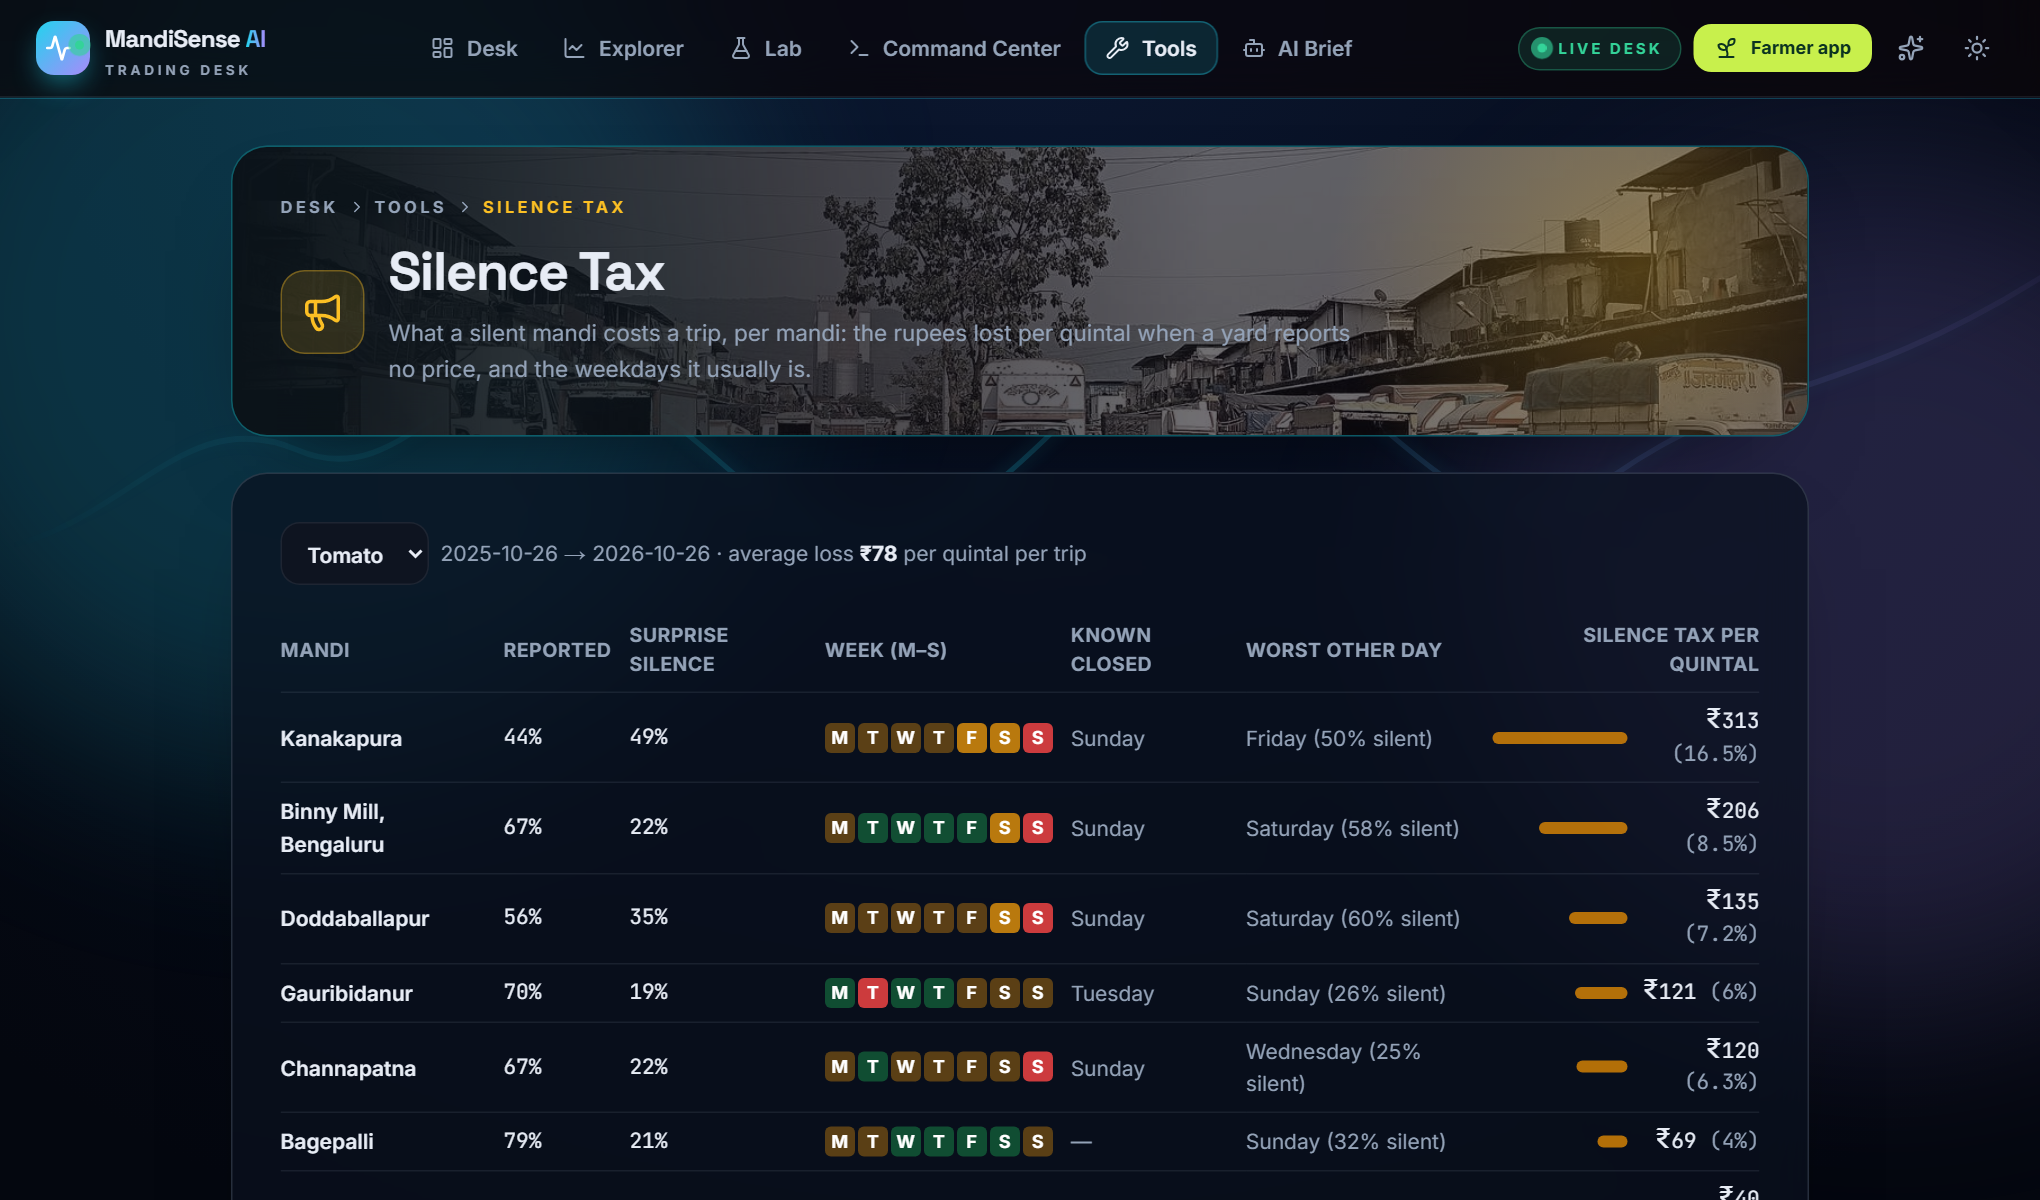
\includegraphics[width=0.93\linewidth]{figures/shot_w_repval.png}}\\[0.5mm]{\footnotesize (a) Reporting value (silence tax): what a market's silence costs}
\medskip
\fbox{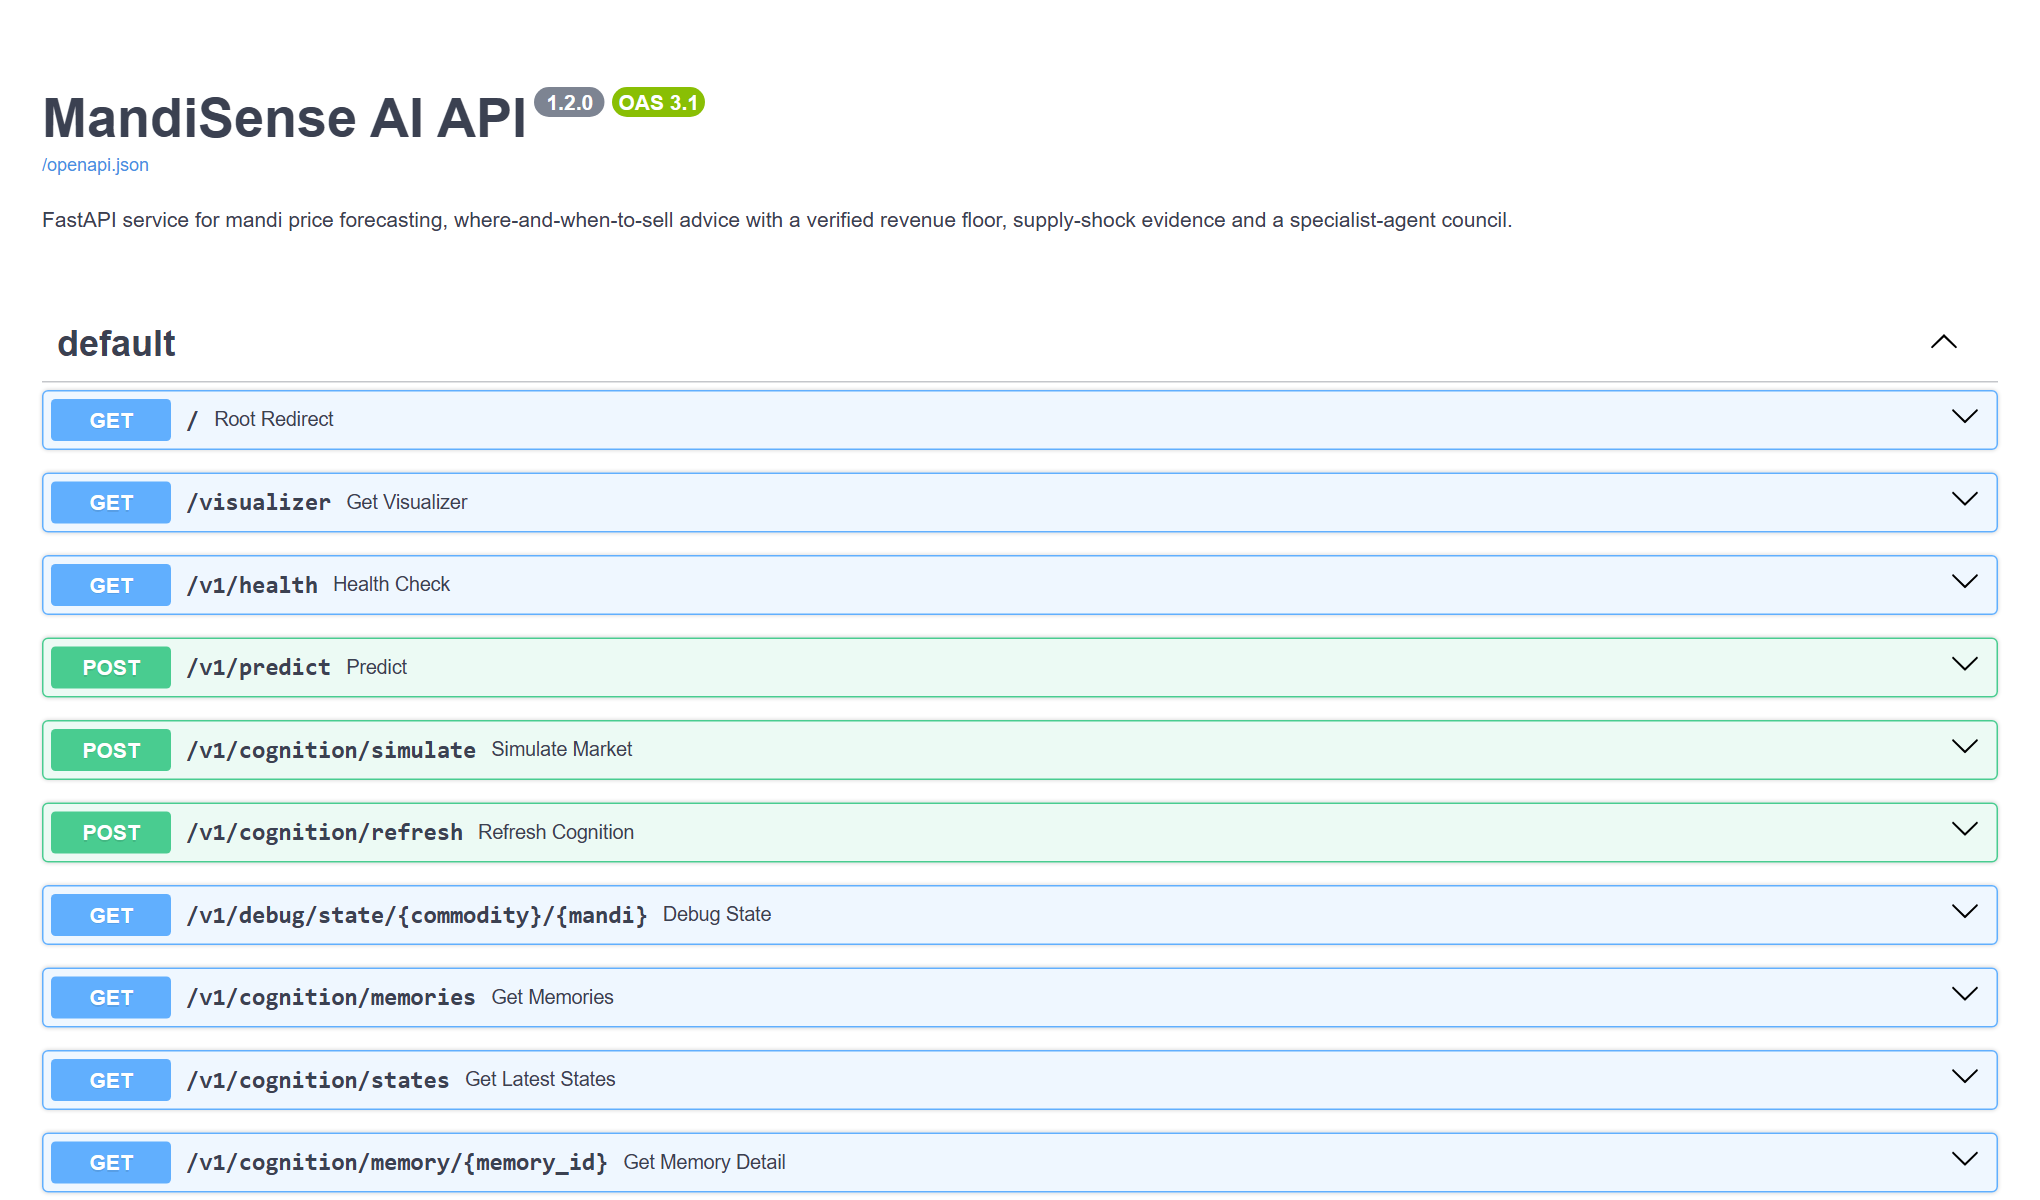
\includegraphics[width=0.93\linewidth]{figures/shot_w_docs.png}}\\[0.5mm]{\footnotesize (b) The interactive API documentation}
\caption{(a) Reporting value (silence tax): what a market's silence costs. (b) The interactive API documentation.}
\label{fig:sc-w-repval}
\end{figure}

The page estimates, per mandi, the revenue lost on days when a market did not report, which is the silence tax of Section~\ref{sec:insight-method}.

Every endpoint is documented automatically from the code, with a form to try it; the service is described in Section~\ref{sec:service-app}.
